% Copyright (c) 2008-2009 solvethis
% Copyright (c) 2010-2018 Casper Ti. Vector
% Public domain.

\documentclass[UTF8]{casthss}
\usepackage{floatrow, amsmath, siunitx, changepage}
\usepackage{booktabs, fancyvrb, forest, multicol}
\usepackage[rmdefault = ntxmi]{isomath}
\usepackage[version = 4]{mhchem}
\usepackage[
	backend = biber, style = caspervector-ay, utf8, cparen,
	sorting = cenyt, giveninits = true, sortgiveninits = true
]{biblatex}

% XXX.
\geometry{top = 2.7cm, bottom = 2.8cm}
\setlength{\hfuzz}{3pt}
\renewcommand*{\ttdefault}{lmtt}
\renewcommand*{\bibfont}{\zihao{5}}
\renewcommand*{\floatpagefraction}{0.75}
\setlength{\bibitemsep}{0pt}
\setlength{\multicolsep}{0pt}
\newcommand*{\bfcmd}{\vspace{0.8em}}
\DeclareFloatFont{cfive}{\zihao{5}}
\floatsetup{heightadjust = all, font = cfive}
\forestset{prune/.style = {text = gray, edge = gray}}
\sisetup{
	math-micro = {\upmu}, text-micro = {\ensuremath{\upmu}},
	math-angstrom = {\text{Å}}, text-angstrom = {Å},
	range-phrase = {--}, range-units = single, group-digits = false
}

\let\cdott\cdot
\renewcommand*{\cdot}{\hspace{-0.03em}\cdott\hspace{0.03em}}
\let\cdotts\cdots
\renewcommand*{\cdots}{\hspace{0.02em}\cdotts\hspace{-0.02em}}
\renewcommand*{\vec}[1]{\vectorsym{#1}}
\newcommand*{\mat}[1]{\tensorsym{#1}}
\newcommand*{\eye}{\mathrm{i}}
\newcommand*{\iee}{\mathrm{e}}
\newcommand*{\dif}{\mathrm{d}}
\newcommand*{\tee}{\mathrm{T}}
\newcommand*{\mccomma}{\text{,}}
\newcommand*{\mcscolon}{\text{;}}
\newcommand*{\mcstop}{\text{。}}
\newcommand*{\myterm}[1]{\textbf{#1}}
\newcommand*{\wyck}[2]{\mathbfit{#2}_\mathbf{#1}}
\newcommand*{\slop}[1]{#1 plus #1 minus #1}
\newcommand*{\cm}[1]{\textcolor{black!66}{#1}}
\newcommand*{\bs}{\char92}
\newcommand*{\lb}{\char123}
\newcommand*{\rb}{\char125}
\newenvironment{rquote}[1]{%
	\par\vspace{\baselineskip}%
	\begin{adjustwidth}{#1}{2\ccwd}%
	\itshape\ifstrempty{#1}{\raggedleft}{}%
}{\end{adjustwidth}}

\RecustomVerbatimEnvironment{Verbatim}{Verbatim}{
	frame = single, obeytabs = true, fontsize = {\zihao{5}},
	baselinestretch = 1.3, commandchars = {\\\{\}}
}
\DeclareFieldFormat{doi}{%
	DOI\addcolon\space\ifhyperref%
		{\href{https://doi.org/#1}{\nolinkurl{#1}}}{\nolinkurl{#1}}%
}
\makeatletter
% XXX.
\def\FV@VerbatimEnd{\FV@EndList\vskip-0.55\baselineskip}
\def\url@sloppystyle{%
	\let\oUrlBreaks\UrlBreaks
	\def\UrlBreaks{%
		\do\a\do\b\do\c\do\d\do\e\do\f\do\g\do\h\do\i\do\j\do\k\do\l\do\m%
		\do\n\do\o\do\p\do\q\do\r\do\s\do\t\do\u\do\v\do\w\do\x\do\y\do\z%
		\do\A\do\B\do\C\do\D\do\E\do\F\do\G\do\H\do\I\do\J\do\K\do\L\do\M%
		\do\N\do\O\do\P\do\Q\do\R\do\S\do\T\do\U\do\V\do\W\do\X\do\Y\do\Z%
		\do\1\do\2\do\3\do\4\do\5\do\6\do\7\do\8\do\9\do\0\oUrlBreaks%
	}%
}
\makeatother

\casthssinfo{
	cthesisname = {博士学位论文}, ethesisname = {dissertation},
	ctitle = {晶体结构测定中正空间法的自动化和性能调优}, etitle = {%
		Automation and Performance Optimisation of the\texorpdfstring{\\}{ }%
		Direct Space Method for Crystal Structure Determination%
	}, cauthor = {刘玙}, eauthor = {Liu Yu},
	cdate = {2018 年 12 月}, edate = {December 2018},
	cmentor = {董成\ 研究员\\(中国科学院物理研究所)},
	ementor = {Prof.\ Dong Cheng},
	cdegree = {理学博士}, edegree = {Doctor of Philosophy},
	cmajor = {凝聚态物理}, emajor = {Condensed Matter Physics},
	cschool = {中国科学院物理研究所},
	eschool = {Institute of Physics, Chinese Academy of Sciences},
	ckeywords =
		{晶体结构测定,正空间法,碰撞检测,增量计算,并行和分布式计算。},
	ekeywords = {%
		Crystal Structure Determination, Direct Space Method,
		Collision Detection, Incremental Computation,
		Parallel and Distributed Computing.%
	}, mentorlines = {2}, confidential = {}
}
\addbibresource{thesis.bib}

\begin{document}
	\frontmatter
	\pagestyle{empty}
	\maketitle
	\cleardoublepage
	\emaketitle
	\cleardoublepage
	\include{chap/origin}

	\cleardoublepage
	\fancypagestyle{plain}{\fancyfoot[C]{\zihao{-5}\normalfont{\thepage}}}
	\pagestyle{plain}
	\setcounter{page}{0}
	\pagenumbering{Roman}
	% Copyright (c) 2014,2016,2018 Casper Ti. Vector
% Public domain.

\begin{cabstract}\raggedbottom
	晶体结构测定的手段可以大致分为倒空间法和正空间法:前者的核心在于提取各衍射峰
	所对应结构因子的振幅,并设法从振幅反推相位,然后通过 Fourier 变换从各衍射峰
	的结构因子得到晶胞内的电子密度分布;后者以晶胞内原子的坐标组合为自变量,
	通过全局最优化算法寻找使计算得到的衍射谱和实际测得的衍射谱最接近的原子坐标。
	和倒空间法相比,正空间法对衍射谱的分辨率要求更低、对衍射峰重叠的容忍度更高,
	因此更加适合处理从粉末衍射得到的数据。在正空间法的求解过程中,对结构中
	成键关系的先验知识可以发挥极大的作用,因此正空间法特别适合求解分子晶体、
	框架晶体等等类型的结构,但其在求解成键关系总体未知的结构时仍然会遇到许多
	困难。为了降低最优化算法中搜索空间的维数,对于后一类型的结构常常可以使用
	等效点系组合(EPC)法:通过将晶胞中的原子分配到可用的 Wyckoff 位置,
	原先以晶胞中所有 $n$ 个原子的坐标为自变量的 $3n$ 维最优化问题可以
	转化为多个互相独立的最优化问题,每个问题以一个 EPC 中独立原子的
	可变坐标为自变量,而且这些最优化问题的维数在多数情况下远小于 $3n$。

	在用正空间法求解晶体结构时,常常会遇到计算的衍射谱和实际谱很接近,但在化学上
	不合理的晶体模型;其中最常见的问题之一是原子重叠,即一些原子对的间距明显小于
	化学上允许的下限。为了尽量自动化地处理原子重叠问题,须要在全局最优化的过程中
	高效地实时检测和排除存在原子重叠的模型;对原子重叠的检测属于计算几何中的
	碰撞检测问题,而我们首先需要的就是一种实时的晶体学碰撞检测算法。本人基于
	碰撞检测中常用的轴对齐包围盒(AABB)模型,并结合晶胞特殊的几何构造,提出了
	一种通用的晶体学碰撞检测算法框架。在此基础之上,针对成键关系总体未知的结构,
	本人对计算几何中常用的 sweep and prune(SAP)算法进行了修改,使之能以
	$O(n\log n)$ 的时间复杂度检测晶体模型中的原子重叠;此外,考虑到这类结构的
	求解往往会使用 EPC 法,本人也提出一种利用等效点系对称性显著减少碰撞检测
	计算量的方法。基于以上的碰撞检测算法,本人设计了一种评估晶胞中
	原子重叠状况的函数,该函数可用于在最优化的过程中实时排除存在原子重叠
	的模型;此外,上述的碰撞检测算法不仅有助于更高效地避免原子重叠,
	而且对于晶胞中配位多面体、原子键价等等的计算也具有重要的意义。

	为了让上文所述的排除原子重叠的机制在求解未知结构的过程中发挥实际的作用,
	本人开发了 \emph{decryst} 这套使用正空间法从粉末衍射数据求解晶体结构的软件。
	\emph{decryst} 在功能上和以前的 \emph{EPCryst} 类似:两者都使用 EPC
	法处理已指标化的数据,并把求解流程分为生成 EPC 列表、对各 EPC 进行统计分析、
	对每个 EPC 进行全局最优化和导出解模型等 4 个主要步骤;因为 EPC 法的缘故,
	两者都特别适合求解成键关系总体未知的结构。和 \emph{EPCryst} 相比,%
	\emph{decryst} 最重要的优势在于后者可以在最优化的过程中利用上文中的机制
	自动、高效地排除原子重叠。此外,受到 Unix 中 \verb|make| 程序的启发,在
	\emph{decryst} 的实现中,本人首次将增量计算的思想以一种具有通用性的方式
	应用于最优化的过程中,使其性能得到了明显的提升;\emph{decryst} 也使用一种
	增量算法生成 EPC,这不仅极大地降低了其内存需求,而且为在生成 EPC 时对其
	进行实时筛选做了准备。为了适应目前科学计算的发展趋势,本人在设计
	\emph{decryst} 时也加入了对并行和分布式计算的支持,使之可以通过同时利用
	多个处理器实现对晶体结构测定的进一步加速。考虑到同一结构的各 EPC 互相独立,
	而且 EPC 数在多数有意义的情形下都相当大,\emph{decryst} 中统计分析和
	全局最优化任务的并行化将为求解成键关系总体未知的结构带来前所未有的机遇。

	\emph{decryst} 是运行在类 Unix 平台上的自由、开源软件,可以从
	\url{https://gitea.com/CasperVector/decryst} 获得;其设计追求简洁、
	灵活,而本人也希望其中的技巧可以在更多的晶体学软件中得到应用。在现有
	自动化工具的配合下,用 \emph{decryst} 能简单地实现相当复杂的求解流程:
	利用重原子法的求解,统计分析和全局最优化后基于 Bragg $R$ 因子的 EPC 筛选,
	求解前筛除必发生原子重叠的 EPC、最优化中实时排除存在原子重叠的晶体模型、
	求解后筛除仍发生原子重叠的 EPC,等等。本文的最后部分讨论了 \emph{decryst}
	的设计和实现,并以美国矿物学家晶体结构数据库(AMCSD)中若干个不同晶系
	和复杂度的结构为例,循序渐进地演示了 \emph{decryst} 的基本用法和常用技巧。
\end{cabstract}

\begin{eabstract}\raggedbottom
	The methods for crystal structure determination can be roughly classified
	into two categories, the reciprocal space methods and the direct space
	method (DSM).  The reciprocal space methods work by extracting the
	amplitudes of structure factors for individual reflections and then phasing
	these reflections, after which the Fourier transform is used to obtain
	the electron density distribution in the unit cell.  In contrast, the DSM
	uses global optimisation (GO) algorithms to minimise the divergence between
	the computed and measured diffraction patterns, and uses the coordinate
	combination of atoms in the unit cell as the variables to be optimised.
	In comparison with the reciprocal space methods, the DSM is more suitable
	for handling low-resolution diffraction data, and is more tolerant of
	overlapping reflection peaks in diffraction patterns.  When using the DSM,
	\emph{a priori} knowledge of the structure to be determined is very
	helpful, so the DSM is quite suitable for structures like molecular crystals
	and framework crystals; on the other hand, it is much more difficult
	to determine structures using the DSM when the bonding relations are
	largely unknown.  To reduce the degree of freedom of the GO problem, the
	equivalent position combination (EPC) method can often be used for the
	latter kind of structures: by assigning the atoms to the available Wyckoff
	positions, we can transform the $3n$-dimensional GO problem with regard to
	all $n$ atoms in the unit cell into multiple mutually independent problems,
	each of which only using the non-fixed coordinates of the independent atoms
	from one EPC, and usually having a degree of freedom much smaller than $3n$.

	In structure determination using the DSM, often encountered are chemically
	unreasonable crystallographic models with the computed diffraction patterns
	very similar to the measured patterns, and one of the top problems is
	atom bumping: in many of these crystallographic models, the distance
	between some atom pairs are unreasonably short.  To automatically handle
	atom bumping, we need to efficiently detect and eliminate crystallographic
	models with atom bumping in real time during the GO procedure;
	since the detection of atom bumping is known as collision detection in
	computational geometry, what we need first is a real-time algorithm
	for crystallographic collision detection.  Based on the axis-aligned
	bounding box (AABB) model, and noticing the unique geometric structure
	of the unit cell, the author proposed a generic framework for
	crystallographic collision detection.  Based on this framework,
	regarding structures with largely unknown bonding relations,
	the author modified the sweep and prune (SAP) algorithm, enabling it to
	detect atom bumping in the unit cell in $O(n\log n)$ time bound.
	In addition, considering that the EPC method is often used in
	determination of these structures, the author proposed a method that
	employs the equivalent position symmetry to significantly reduce the
	computational complexity of collision detection.  Based on these algorithms,
	the author designed an evaluation function for atom bumping in
	crystallographic models, which can be used to eliminate unreasonable models
	in real time during the GO procedure; additionally, apart from the
	prevention of atom bumping, the collision detection algorithms mentioned
	above can also be very helpful in computation of coordination polyhedra,
	valence, \emph{etc.}\ in crystallographic models.

	To facilitate practical use of above-mentioned mechanisms in
	determination of unknown structures, the author wrote \emph{decryst},
	a software suite for structure determination from powder diffraction that
	uses the DSM.  \emph{decryst} is functionally similar to \emph{EPCryst}:
	both use indexed data, employ the EPC method and abstract structure
	determination as 4 stages, enumerating EPCs, statistical analyses of EPCs,
	GO of EPCs and exporting the results; and due to the EPC method, both are
	particularly suitable when the bonding relations are largely unknown.
	The most important advantage of \emph{decryst} over \emph{EPCryst} is that
	the former can automatically and efficiently eliminate atom bumping.  In
	addition, inspired by the \verb|make| utility from Unix, the author employed
	incremental computation in a generic way, for the first time, in the GO
	procedure, resulting in a dramatic speedup of the procedure; \emph{decryst}
	also employs an incremental algorithm for the generation of EPCs, allowing
	for real-time filtering during the generation procedure in the future.  In
	order to accommodate for contemporary developments in scientific computing,
	the author designed \emph{decryst} with parallel and distributed computing
	in mind, allowing for further enhancement of the performance by simultaneous
	use of multiple processors.  Noticing that EPCs are mutually independent,
	and that the number of EPCs is large in most useful cases, it is expected
	that the parallelisation of statistical analyses and GO of EPCs will offer
	unprecedented opportunities for determination of structures with largely
	unknown bonding relations.

	\emph{decryst} is free and open source software that
	runs on Unix-like platforms, and can be obtained from
	\url{https://gitea.com/CasperVector/decryst};
	it is designed to be simple and flexible, in the hope that the underlying
	techniques could be adopted in more crystallographic applications.
	In combination with well-established automation utilities, it is easy to
	implement fairly complicated structure determination procedures:
	the heavy-atom method, filtering of EPCs based on the Bragg $R$ factor
	after statistical analyses and GO; filtering of EPCs that would definitely
	produce crystallographic models with atom bumping before actually solving
	the structure, real-time elimination of models with atom bumping in GO,
	filtering of EPCs that have atom bumping in the solutions, \emph{etc}.
	The final parts of this dissertation discussed the design and
	implementation of \emph{decryst} and then demonstrated its basic usage
	and some useful techniques, using example structures from various
	crystal families and of varying complexities, that are taken from the
	American Mineralogist Crystal Structure Database (AMCSD).
\end{eabstract}

% vim:ts=4:sw=4

	\tableofcontents
	\listoffigures
	\listoftables

	\mainmatter
	\fancypagestyle{plain}%
		{\fancyfoot{}\fancyfoot[LE,RO]{\zihao{-5}\normalfont{\thepage}}}
	\pagestyle{plain}
	% Copyright (c) 2014,2016,2018 Casper Ti. Vector
% Public domain.

\chapter{引言}
\section{晶体和 X 射线的相互作用}

在 \textcite{rietveld1969}关于全谱拟合的工作之后,晶体结构解析常常被分为
结构测定和结构精修两个主要步骤:前者对空间群、晶胞参数、晶胞化学式和
原子坐标等等基本参数进行大致的确定,而后者不仅对这些参数进行精细的调整,
而且也对由仪器灵敏度、衍射峰形等等更多因素决定的各种参数进行拟合,
以使所有这些参数和实际测得的整个衍射谱之间达到最大程度的吻合。
本文主要讨论通过 X 射线粉末衍射测定晶体结构的问题,
而本节将对晶体和 X 射线之间相互作用的理论进行简要的总结。

一般而言,在对晶体样品进行 X 射线衍射实验时,光源、检测器到样品的距离都远大于
样品的尺寸,而 X 射线的波长和晶胞的尺寸在相近的数量级上,因此样品对 X 射线的
散射满足 Fraunhofer 远场条件\parencite{zhong2003}。晶体和 X 射线之间的相互
作用主要是其中电子云对 X 射线的散射,而在电子云对单波长电磁波的远场散射中,
散射波的复振幅 $A$ 和散射体的电子密度分布 $\rho$ 之间满足以下的 Fourier 关系:
\begin{equation}
	A(\vec{q}) \propto f(\vec{q}) = \int\rho(\vec{r})
		\iee^{2\uppi\eye\vec{q}\cdot\vec{r}}\dif\tau_\vec{r}\mccomma
\end{equation}
其中 $\vec{q}$ 为散射向量,$\tau_\vec{r}$ 为正空间的体积元,$f$ 即%
\myterm{散射因子}。由此结合 Fourier 变换的可加性和位移{--}相移关系,
并忽略 X 射线的次级散射\parencite[4]{pecharsky2009},
可知原点在 $(0, 0, 0)$ 的单个晶胞的散射因子正是其\myterm{结构因子}
\begin{equation}
	F(\vec{q}) = \sum_j f_j(\vec{q})
		\iee^{2\uppi\eye\vec{q}\cdot\vec{r}_j}\mccomma
\end{equation}
其中 $j$ 为单个原子\footnote{%
	在讨论晶体结构时,常常将其中的离子也称为“原子”,而本文中也采用这一约定。%
}的编号,$f_j$ 和 $\vec{r}_j$ 分别为其原子散射因子和坐标。

再次在忽略次级散射后利用 Fourier 变换的可加性和位移{--}相移关系,
可得整块晶体的散射因子为
\begin{equation}
	\sum_j F(\vec{q})\iee^{2\uppi\eye\vec{q}\cdot\vec{r}_j}
	= F(\vec{q})\sum_j\iee^{
		2\uppi\eye(h\vec{a}^* + k\vec{a}^* + l\vec{a}^*)
		\cdot(u_j\vec{a} + v_j\vec{b} + w_j\vec{c})
	} = F(\vec{q})\sum_j\iee^{2\uppi\eye(hu_j + kv_j + lw_j)}
	\mccomma\label{eq:amp-sf}
\end{equation}
其中 $\{\vec{a}, \vec{b}, \vec{c}\}$、$\{\vec{a}^*, \vec{b}^*, \vec{c}^*\}$
分别为正空间和倒空间晶格的基向量组\footnote{%
	本文统一使用不含 $2\uppi$ 因子的倒基向量定义%
	\parencite[1]{prince2004},以下不再特别说明。%
},$j$ 为单个晶胞的编号,$\vec{r}_j$ 为该晶胞的原点坐标。假设有一个
晶胞的原点在 $(0, 0, 0)$,那么为了使来自所有晶胞的散射波发生相长干涉,%
$hu_j + kv_j + lw_j$ 应均为整数;又由晶体\footnote{%
	国际晶体学联合会\parencite{iucr1992}目前将晶体定义为“any solid having
	an essentially discrete diffraction diagram”,即包括具有平移周期性的
	常规晶体和不具有平移周期性的准晶\parencite{shechtman1984};然而,
	本文只讨论常规晶体的结构测定,而本文所称的“晶体”也一律指常规晶体。%
}的平移周期性可知 $u_j$、$v_j$、$w_j$ 均为整数,因此 $h$、$k$、$l$ 也应为整数。

由此可知,产生衍射峰的散射向量必须是倒晶格向量,这正是我们熟知的 Laue 条件;
在满足 Laue 条件时,由 (\ref{eq:amp-sf}) 式进一步可知总散射因子正比于
结构因子。在具体的衍射实验中,还有其它的许多因素影响实际测得的衍射谱%
\parencite{liang2011}:例如衍射装置的几何结构主要由 Lorentz{--}极化因子
反映,粉末衍射中倒易向量模相等的衍射峰互相重叠由多重度因子反映,此外还有
热振动、样品吸收等等多种影响因素。但无论如何,由本节的推导可见,结构因子和
晶胞中原子排布之间的紧密联系决定了对结构因子的处理是晶体结构测定的核心。

\section{倒空间法求解晶体结构}\label{sec:reci-meth}

因为 Fourier 变换具有可逆性,如果获得了各主要衍射峰所对应结构因子的值,
就可以通过逆变换获得晶胞内的电子密度分布,从而得到晶胞内各原子的位置;
然而在进行衍射实验时,对 X 射线的测量会丢失相位信息,因为仪器测量到的只是
衍射峰的强度,而其正比于结构因子振幅的平方。因此如果要得到完整的结构因子,
就须要设法重建结构因子的相位,而重建结构相位的数值依据就是结构振幅。
这正是结构测定中\myterm{倒空间法}的基本思路,其名字源于对倒空间中结构振幅
的提取;以下对目前在用粉末衍射数据进行结构测定\parencite{david2002}%
的算法中被最广泛使用的几种倒空间法进行简要的总结,其中各方法的
常用软件列表可以参考下文中相应的文献。

\myterm{Patterson 法}\parencite{rossmann2001}:
对结构振幅的平方(正比于衍射峰的强度)进行 Fourier 变换,可以得到
Patterson 函数,后者可以理解为电子密度分布的自卷积或“自关联”函数
\begin{equation}
	P(\vec{R}) = \int\,\rho(\vec{r})\rho(\vec{r + R})\dif\tau_\vec{r}\mcstop
\end{equation}
含 $n$ 个原子的晶胞会在 Patterson 函数中产生 $n^2$ 个峰,
因此即使不考虑峰的重叠问题,一般而言总的 Patterson 峰数仍然会很大。
除了原点处的强峰之外,具有高强度的 Patterson 峰主要由含重原子的原子对产生,
所以由这些重原子峰可以确定重原子的位置,而由重原子的位置结合
Patterson 函数中更多的信息便可以进一步推测整个晶胞中各原子的位置。

\myterm{直接法}\parencite{giacovazzo2001}:
根据电子密度分布函数的正定性和原子性,可以得到不同衍射峰所对应
(为抵消高角度峰的强度衰减)归一化结构因子 $E_\vec{q}$ 以及单位结构因子
$U_\vec{q}$ 之间的一系列数值关系,其中最重要的是一组根据给定衍射峰的
结构振幅对一些相关衍射峰结构相位的取值进行限制的不等式关系,
以及一组概率性的等式关系:例如对 $P\bar1$ 空间群有
\vspace{\slop{-0.05em}}
\begin{equation}
	U_\vec{q} ^ 2 \leq (1 + U_{2\vec{q}}) / 2\mccomma
	\vspace{\slop{-0.05em}}
\end{equation}
而以下的正切公式(其中 $G_\vec{k} \propto
|E_\vec{q}||E_\vec{k}||E_{\vec{q}-\vec{k}}|$)给出最概然的结构相位
\vspace{\slop{0.09em}}
\begin{equation}
	\tan\arg{E_\vec{q}} = \frac%
	{\sum_\vec{k} G_\vec{k} \sin(\arg{E_\vec{k}} + \arg{E_{\vec{q}-\vec{k}}})}%
	{\sum_\vec{k} G_\vec{k} \cos(\arg{E_\vec{k}} + \arg{E_{\vec{q}-\vec{k}}})}
	\mcstop
	\vspace{\slop{0.09em}}
\end{equation}
在实际求解时,在计算 $E_\vec{q}$、$U_\vec{q}$ 后,选出较强衍射峰所组成的
$\{\vec{q}, \vec{k}, \vec{q}-\vec{k}\}$ 三元组,根据上述的不等式和等式关系
可以对其中一小部分结构相位的符号甚至具体数值进行直接估计;在此之后,通过
迭代性地应用等式关系和不等式关系,就可以对各主要衍射峰的结构相位进行重建。

\myterm{电荷反转法}\parencite{palatinus2013}:
在满足 Friedel 定律\parencite[218-220]{pecharsky2009}的前提下,
如果对各结构因子赋予随机相位,由此得到的电子密度分布往往不具备正定性
和原子性。为了满足正定性条件,可以强行将负电子密度部分的符号反转;
此外为了引入随机微扰,考虑到实际电子密度分布的集中性(可以认为是
由原子性导致的),实际计算时会将电子密度小于某一预设正值的部分进行
反转。在这样修改电子密度分布之后,用原结构振幅结合反演得到的结构相位,
得到的结构因子又可以通过同样的流程产生新的结构相位,如此便可进行迭代;
根据实际测试,对于许多衍射谱,通过上述迭代算法可以获得满意的结构相位。

一般而言,为了能使用倒空间法正确求解晶体结构,衍射谱中可确定结构振幅的
衍射峰数须要远多于晶胞中待定的原子数,因此衍射数据通常需要较高的分辨率,
这在上述几种算法的参考文献中多少有所提及。在对粉末衍射数据使用倒空间法时,
还须要设法分离互相重叠的衍射峰,这又使得粉末数据需要比单晶数据更高的分辨率。
在很多情况下,高分辨的衍射数据很难获得,特别是对纳米材料,即使应用
同步辐射也很难获得高质量的单晶衍射数据;在没有高分辨衍射数据的情况下,
常常不得不使用正空间法求解晶体结构,而正空间法就是本文将要讨论的主题。

\section{正空间法和等效点系组合法}\label{sec:dspace-epc}

求解晶体结构的另一种主要思路是直接从原子坐标建立试探性的晶体模型,然后计算
晶体模型所对应的衍射谱,将计算得到的衍射谱和实际测得的衍射谱比对,并根据结果
设法对晶体模型进行优化,直到获得满意的模型。这正是\myterm{正空间法}%
\parencite{cerny2007}的思路,后者是除了上文中讨论的倒空间法之外,
用粉末衍射数据进行结构测定的主要算法;显然,正空间法并不依赖对结构相位的估计,
而且甚至不需要单个衍射峰的结构振幅,因此其特别适合处理低分辨的衍射数据,
以及衍射峰重叠严重的粉末数据。

在计算机尚未被广泛应用于科学计算的年代,晶体结构测定仍严重依赖手动计算和尝试,
而对于晶体模型的优化也极大程度地依赖具有极强技巧性(乃至艺术性)的人工处理:
例如在包括\textcite{lu1965},\textcite{reddy1965}在内的许多先驱的工作中,
晶体学家在大致确定各原子的等效点系组合(参考下文和第 \ref{ssec:epc-discus}
小节)之后,通过立体几何的原理确定具体的原子坐标。在现代的正空间法中,
尝试性晶体模型的建立和优化仍然不可或缺,只是往往被自动化的计算机程序
以极高的频率反复进行;因为这样的原因,正空间法也往往被称为尝试法%
\parencite{wolfson1997}和模型法\parencite{cerny2007}。

从数学上容易看出,正空间法将结构测定抽象为寻找使一%
\myterm{目标函数}最小化的原子坐标组合
\begin{equation}
	\mat{x} = (x_1, y_1, z_1, x_2, y_2, z_2, \cdots, x_n, y_n, z_n)^\tee
\end{equation}
的全局最优化问题,其中 $n$ 是晶胞内的原子数,而目标函数中最重要的部分是
表征计算谱和实际谱之间差异的 \myterm{Bragg $R$ 因子}。为了利用计算机
自动化地寻找合理的 $\mat{x}$,现代的正空间法使用各种最优化算法,
例如模拟退火\parencite{david2006}、并行回火\parencite{cerny2007}、
遗传算法\parencite{shankland1997}等等来求解上述的问题,
因此正空间法的另一个别称是全局最优化法\parencite[252]{david2002}。

若直接以晶胞中所有 $n$ 个原子的坐标组合为正空间法中全局最优化的自变量,
则最优化问题的维数为 $3n$;注意到最优化问题中搜索空间的规模随其维数指数增长,
设法尽量降低维数显然很有必要。对于成键关系大部分已知的结构,例如分子晶体%
\parencite{andreev1997}、框架晶体\parencite{falcioni1999}以及部分其它类型的
晶体\parencite{favre2002},可以将原子团的平移、振动、转动等等自由度作为自变量,
利用原子团的相对刚性来降低最优化问题的维数,并对键长、键角进行适当限制以进一步
缩小搜索空间。相比之下,在求解成键关系总体未知的结构时,关于成键关系的
先验知识就缩小搜索空间而言作用很有限;对于这类结构,等效点系组合法%
\parencite{deng2009}常常是一种有效的手段,而下文就将对其进行简要的总结。

在空间群和晶胞化学式已知\footnote{%
	本文主要考虑对已指标化粉末衍射数据的处理,因此在讨论结构测定时一般假定
	晶胞参数和空间群是已知的,或至少能确定空间群在某个比较小的范围之中。此外,
	因为结构测定所用样品的名义组成一般是已知的,在确定晶胞参数之后常常可以
	通过密度测量获得晶胞的化学组成,所以本文一般也假定晶胞化学式是已知的。%
}的前提下,考虑到绝大多数晶体中晶胞的对称性,可以将晶胞中独立原子的坐标
作为自变量,从而极大地降低最优化问题的维数。为了得到独立原子的具体列表,
我们须要将晶胞中的原子分配到可用的 Wyckoff 位置上,而每一种分配方案就是一种%
\myterm{等效点系组合}(equivalent position combination,简称 EPC)。例如对于
\ce{PbSO4}($Pnma$,$Z = 4$),因为 $Pnma$ 空间群有 $4a$、$4b$、$4c$、$8d$
等共 4 种 Wyckoff 位置,为了满足正确的晶胞化学式,其中原子有且仅有 35 种 EPC:
\vspace{\slop{0.15em}}
\begin{itemize}
	\item \ce{Pb^{2+}}: $4a\times1$; \ce{S^{6+}}: $4b\times1$;
		\ce{O^{2-}}: $4c\times4$(8 维);
	\item \ce{Pb^{2+}}: $4a\times1$; \ce{S^{6+}}: $4b\times1$;
		\ce{O^{2-}}: $4c\times2 + 8d\times1$(7 维);
	\item ……
	\item \ce{Pb^{2+}}: $4c\times1$; \ce{S^{6+}}: $4c\times1$;
		\ce{O^{2-}}: $4c\times2 + 8d\times1$(11 维,正确 EPC)。
	\item \ce{Pb^{2+}}: $4c\times1$; \ce{S^{6+}}: $4c\times1$;
		\ce{O^{2-}}: $8d\times2$(10 维)。
\end{itemize}
\vspace{\slop{0.15em}}
原先 72 维的最优化问题被转化为 35 个介于 6--12 维之间的最优化问题,
可见 EPC 法极大地缩减了 \ce{PbSO4} 结构求解问题的总规模。

正空间法和 EPC 法的常用软件列表参考第 \ref{sec:atom-bump} 小节;此外有必要指出,
随着近年来双空间迭代技术,如电荷反转法(参考第 \ref{sec:reci-meth} 节),%
\textcite{altomare2008b}的直接法{--}模拟退火混合方案和 \textcite{ma2004}的
UACIEM 方法等等的发展,倒空间法和正空间法之间的界限正在逐步地模糊。然而,
双空间迭代法目前的发展趋势并非是取代倒空间法或正空间法,而是让这两类算法
更加紧密地互相结合,因此针对后两类算法本身的研究仍然是具有重要意义的。

\section{原子重叠问题和 \emph{decryst}}\label{sec:atom-bump}

正空间法遇到的一个重要问题是随机产生的晶体模型在化学上不合理,而其中最常见的情况
之一是\myterm{原子重叠}(atom bumping),即产生的模型中一些原子对的间距明显小于
化学上允许的下限,而且这些模型中一部分甚至具有和正确模型相近的 Bragg $R$ 因子。
例如对于 \ce{PbSO4} 的正确等效点系组合(EPC),如果试图通过最小化 $R$ 因子来
求解原子坐标,最终得到的结果往往类似于图 \ref{fig:pso-bump}:虽然正确的
晶体模型中没有原子重叠,但是绝大部分解模型中有严重的原子重叠。对于成键关系
大部分已知的结构,通过对键长、键角等等参数的限制,可以极大地减轻这一问题;
然而对于成键关系总体未知的结构,这一方法的效果很有限。因此为了尽量自动化地
处理原子重叠,我们迫切需要一种具有通用性的机制在全局最优化的过程中高效地
实时检测和排除存在原子重叠的模型,而本文第 \ref{chap:cryst-cd} 章将要
讨论的就是本人\parencite{liu2017}提出的自动化排除原子重叠的机制。

\begin{figure}[htbp!]\bfcmd
\ffigbox{\begin{subfloatrow}[3]
	\ffigbox[\FBwidth]{%
		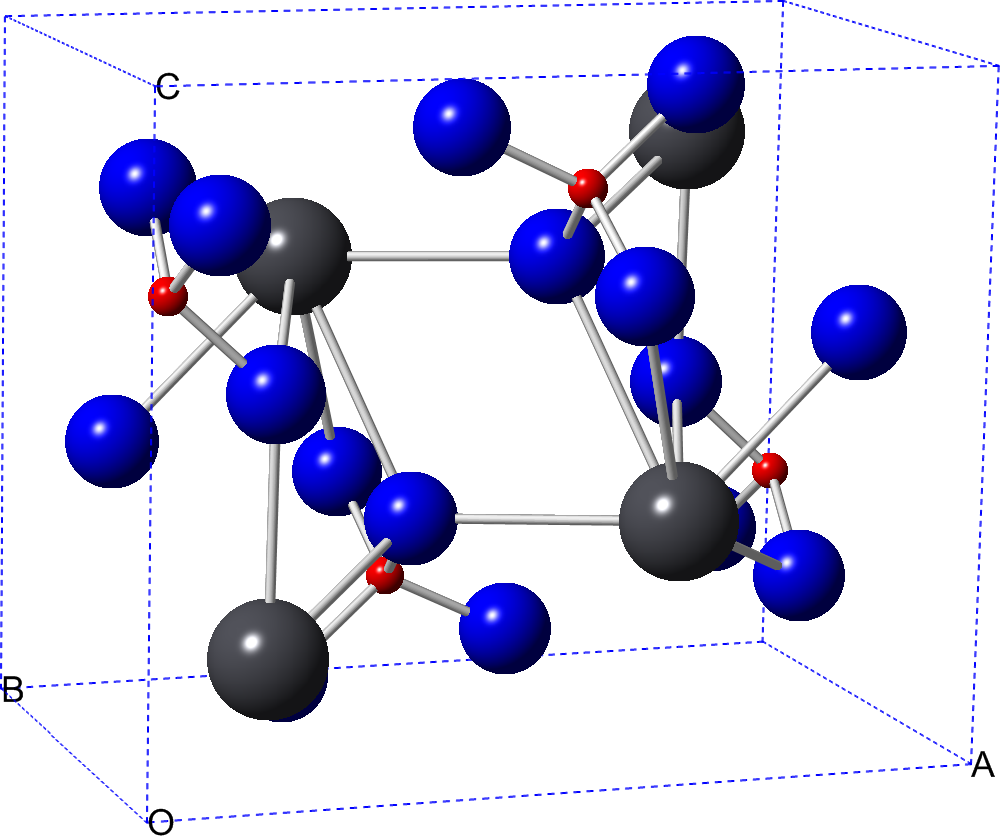
\includegraphics[width = 0.3\textwidth]{img/pso-bump-1}%
	}{\caption{$R = 0.1285$}}
	\ffigbox[\FBwidth]{%
		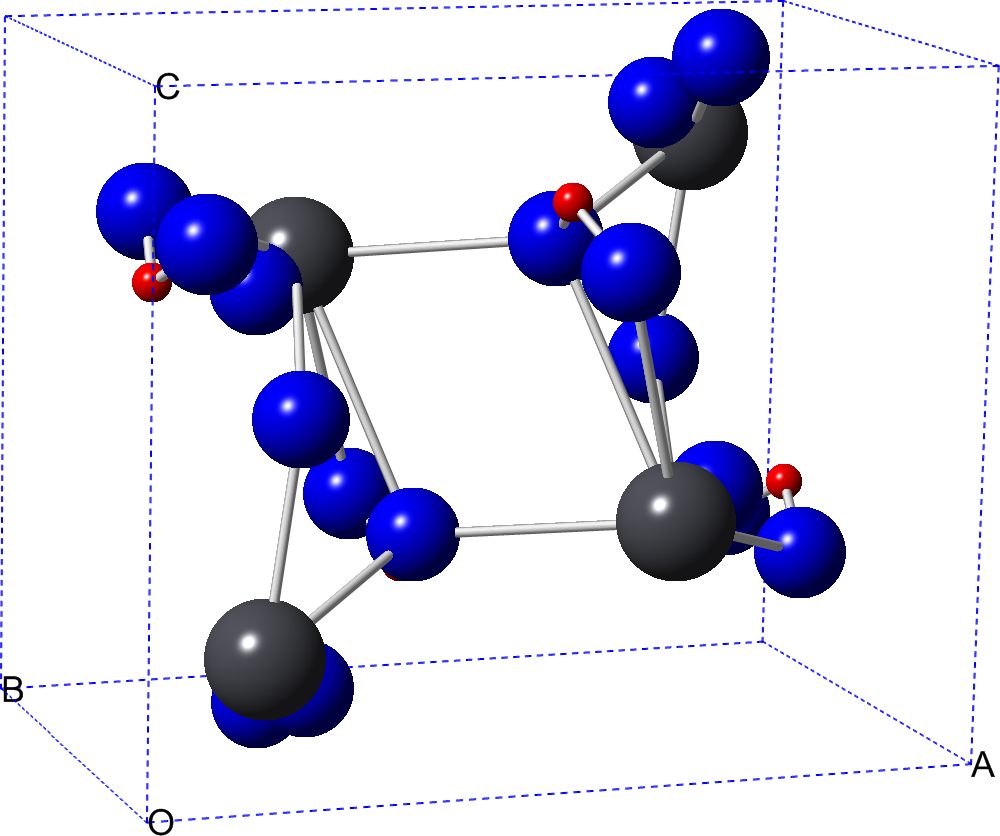
\includegraphics[width = 0.3\textwidth]{img/pso-bump-2}%
	}{\caption{$R = 0.0971$}}
	\ffigbox[\FBwidth]{%
		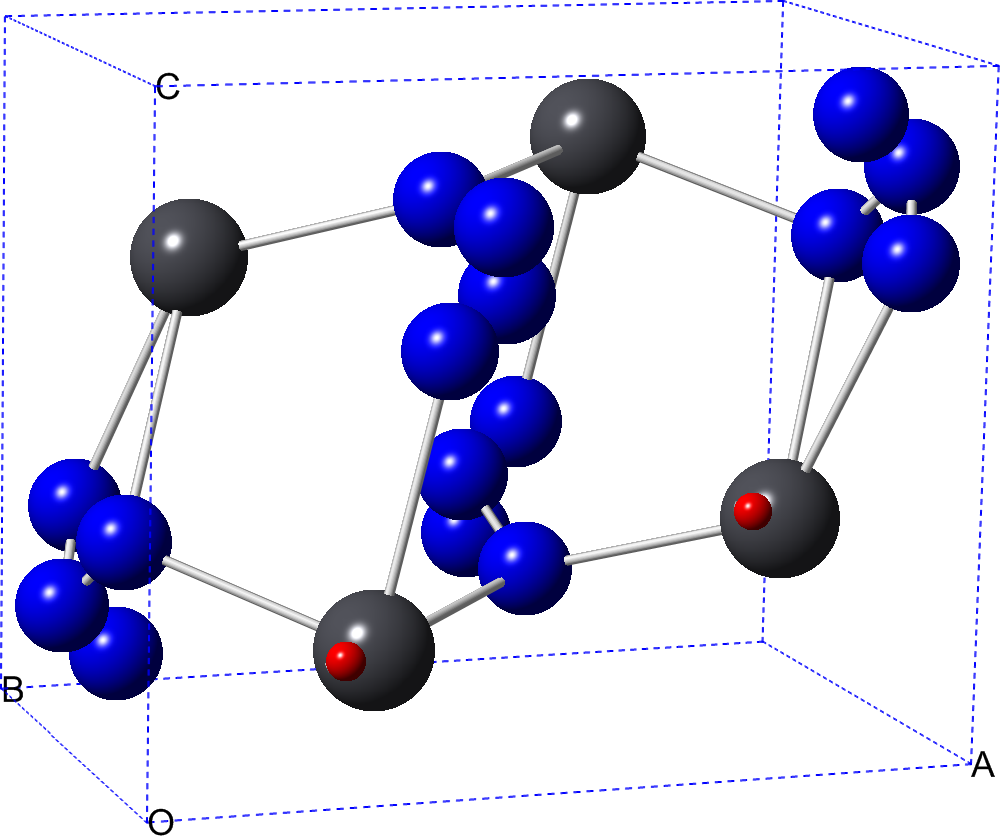
\includegraphics[width = 0.3\textwidth]{img/pso-bump-3}%
	}{\caption{$R = 0.1140$}}
\end{subfloatrow}}{\caption[\ce{PbSO4} 的几种晶体模型]{%
	\ce{PbSO4} 的几种晶体模型,其中只有 (a) 正确
	(数据来源参考第 \ref{ssec:cd-eval} 小节)%
}\label{fig:pso-bump}}
\end{figure}

现有的使用正空间法从粉末衍射数据求解晶体结构的主流软件,如 \emph{FOX}%
\parencite{favre2002}、\emph{DASH}\parencite{david2006}、\emph{EXPO}%
\parencite{altomare2013}等等多数适合求解成键关系大部分已知的结构,但在求解
成键关系总体未知的结构时不甚有效;针对后一类结构的求解,\textcite{deng2011}%
基于 EPC 法开发了 \emph{EPCryst} 这一软件,但其对原子重叠的处理方式是在
全局最优化步骤完成之后对解模型进行筛选,因此排除原子重叠的效率相当低。
考虑到以上的现状,本人开发了 \emph{decryst}\parencite{liu2018},
以使上述的排除原子重叠的机制在求解未知结构的过程中发挥实际的作用。

受 Unix 中 \verb|make| 程序\parencite{feldman1979}的启发,本人在
\emph{decryst} 中将增量计算的技术应用于最优化步骤中,使其性能得到了很大的提升;
除此之外,考虑到目前科学计算(乃至通用计算)中大规模并行化的发展趋势,
本人在设计 \emph{decryst} 时也加入了对并行和分布式计算的支持,
使之可以通过同时利用多个处理器实现对晶体结构测定的进一步加速。
因为各 EPC 在计算上互相独立,而多数未知结构的 EPC 数很大,
可以认为 EPC 法对搜索空间的缩减作用和 EPC 任务的大规模并行化将为
求解成键关系总体未知的结构带来前所未有的机遇。针对这些内容,本文第
\ref{chap:decr-theory} 章将展开讨论 \emph{decryst} 的基本设计和实现。

第 \ref{sec:dspace-epc} 节提到,在早期的利用正空间法进行结构测定的工作中,
晶体学家通过具有很强经验性和技巧性的手段对备选的 EPC 进行分析,从而筛除掉其中
不可能产生合理晶体模型的 EPC。在 \emph{EPCryst} 中,用户可以通过对随机晶体模型
Bragg $R$ 因子的统计分析实现对 EPC 的简单筛选;在此基础之上,\emph{decryst}
在筛选 EPC 时使用包含原子重叠的目标函数,因此可以在筛选中同时考虑 $R$ 因子和
原子重叠两种因素。\emph{decryst} 的设计追求简洁、灵活,其在现有自动化工具
的配合之下可以实现相当复杂的求解流程,如重原子法和多步骤的精细 EPC 筛选。
针对以上问题,本文第 \ref{chap:decr-usage} 章将比较详细地讨论 \emph{decryst}
的使用方法和常用技巧。

最后有必要指出,除了 EPC 法之外,\emph{FOX} 中的动态占据率校正(dynamical
occupancy correction)也是一种处理特殊位置上原子的有效方法,但其更适用于
以原子团为基础的晶体模型。对于成键关系总体未知的结构,该方法就降低最优化
问题的复杂度而言效果有限,因此在实用性上不如 EPC 法。

\begin{rquote}{0.2\textwidth}
	Zum Nutzen und Gebrauch der Lehrbegierigen
	Musicalischen Jugend, als auch derer in diesem
	studio schon habil seyenden besonderem Zeitvertreib [...]
\end{rquote}
\rightline{--- J.\ S.\ Bach, ``\emph{Das Wohltemperierte Klavier}''}

% vim:ts=4:sw=4

	% Copyright (c) 2014,2016,2018 Casper Ti. Vector
% Public domain.

\chapter{晶胞中原子重叠的实时检测和排除}\label{chap:cryst-cd}
\section{晶体学粗碰撞检测}

对物体重叠的检测属于计算几何中的\myterm{碰撞检测}(collision detection)问题%
\parencite{ericson2005},所以为了在全局最优化中高效地实时检测和排除存在原子重叠
的晶体模型,首先需要的就是一种实时的晶体学碰撞检测算法。对于含 $n$ 个原子的晶
胞,如果通过直接逐对计算原子间距来检测重叠,那么就须要计算所有 $n (n - 1) / 2$
个原子对的间距,因此算法的时间复杂度为 $O(n^2)$ 量级;由此可见 $n$ 较大时逐对
算法在性能上是不利的,而这一问题也是实现实时碰撞检测的主要障碍之一。为了解决
这一问题,实际的碰撞检测通常被分为\myterm{粗碰撞检测}(broad phase)和%
\myterm{细碰撞检测}(narrow phase)两个步骤\parencite[329]{ericson2005}:
前者排除那些明显不会发生碰撞的物体对,而后者对剩下的物体对进行精确的测试
以判断其是否发生碰撞。本节主要就粗检测展开讨论。

\subsection{晶胞的几何构造}\label{ssec:cryst-geom}

对于直角坐标系下的低维 Euclid 空间,碰撞检测是较为成熟的研究领域;然而晶胞有其
独特的几何构造,这使我们难以在晶胞中原封不动地应用现有的碰撞检测算法。首先的
问题是晶胞的 $a$、$b$、$c$ 轴在很多情况下并不互相正交,因此在晶胞中常常不便使用
直角坐标系;针对这一问题,晶体学家的惯用对策是使用分数坐标。假设晶胞中某位移向量
$\vec{x}$ 的分数坐标为 $\mat{x} = (x, y, z)^\tee$,则其 Cartesian 坐标为
\begin{equation}
	\mat{r} = x\mat{a} + y\mat{b} + z\mat{c}
	= \big(\mat{a}\ \mat{b}\ \mat{c}\big) {
		\renewcommand*{\arraystretch}{0.66}
		\begin{pmatrix} x \\ y \\ z\\\end{pmatrix}
	} = \mat{A}\mat{x}\mccomma
\end{equation}
其中 $\mat{a}$、$\mat{b}$、$\mat{c}$ 为正空间各基向量的 Cartesian 坐标。
可见坐标变换矩阵 $\mat{A}$ 正是基向量组矩阵,且进一步可知 $\vec{x}$ 的长度为
\begin{equation}
	\mat{r}^\tee\mat{r} = \mat{x}^\tee\mat{A}^\tee\mat{A}\mat{x}
	= \mat{x}^\tee\mat{G}\mat{x}\mccomma
\end{equation}
其中二次型 $\mat{G} = \mat{A}^\tee\mat{A}$ 正是分数坐标下以矩阵形式表示的
晶胞度规张量\parencite[66]{dodson1991},而后者决定了晶胞中的距离构造。
在分数坐标下,晶胞中的原子位置可以用 3 个互相独立的坐标 $x$、$y$、$z$ 表示;
又因为每个坐标分别满足周期边界条件,即它们各是一个一维圆环 $S^1$ 上的坐标,
所以分数坐标下的晶胞事实上是被建模为 3 个一维圆环的 Cartesian 积(类似于图
\ref{fig:torus-period} 中的情形),即一个三维环面 $T^3$%
\parencite{choquet2009},而这个三维环面具有上述的特殊距离构造。

\begin{figure}[htbp!]\bfcmd
\ffigbox{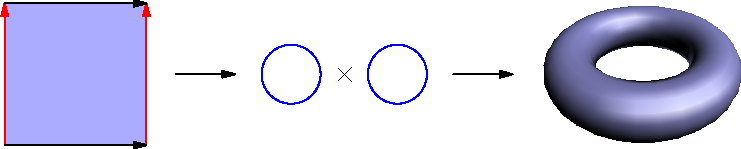
\includegraphics[width = 0.7\textwidth]{img/torus-period}}{\caption{%
	二维晶胞建模为二维环面:$S^1 \times S^1 = T^2$%
}\label{fig:torus-period}}
\end{figure}

粗碰撞检测中一种很普遍的做法是围绕每个被检测的物体构造一个包围体%
\parencite[75-123]{ericson2005},然后利用包围体的特定几何属性来进行优于
$O(n^2)$ 的粗检测;一种常用的包围体是\myterm{轴对齐包围盒}(axis-aligned
bounding box,简称 AABB),即以物体在各坐标轴上的投影区间为边界的盒子(图
\ref{fig:aabb-frac})。两个 AABB 间发生碰撞当且仅当其在 3 个坐标轴上的投影区间
均发生碰撞,因此使用 AABB 在很多时候可以将三维问题化为 3 个一维问题;注意到这里
应用的是变量分离的数学思想,而在晶胞内用分数坐标正好可以实现 3 个坐标的分离,
在使用 AABB 对晶胞内原子进行粗检测时使用分数坐标显然是最合适的选择\footnote{%
	此外,因为上述的 AABB 碰撞判据只涉及对投影区间上下界的比较而不涉及距离,
	所以分数坐标下晶胞的特殊距离构造并不影响 AABB 的使用。%
}。最后,为了能使用 AABB 进行粗检测,还须要解决计算 AABB 的问题:具体而言,
给定原子的分数坐标和 Cartesian 半径 $r$,如何计算其在分数坐标下的 AABB?

\begin{figure}[htbp!]\bfcmd
\ffigbox%
	{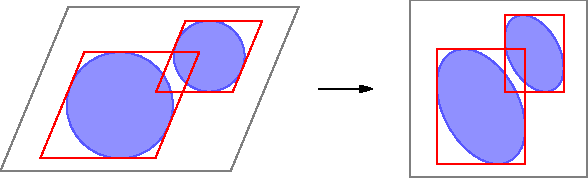
\includegraphics[width = 0.6\textwidth]{img/aabb-frac}}%
	{\caption{轴对齐投影和分数坐标下 AABB 的等价性}\label{fig:aabb-frac}}
\end{figure}

考虑到分数坐标下使用 AABB 正好等价于在以 $a$、$b$、$c$ 轴为坐标轴的仿射坐标下
使用和坐标轴对齐的斜投影(图 \ref{fig:aabb-frac}),不妨从一个和 $a$ 轴及 $a^*$
轴均正交(因此也和 $bOc$ 平面平行)的方向考察上述原子在 $a$ 轴上的轴对齐投影
(图 \ref{fig:aabb-width-1}),此时只须计算投影区间的半宽 $R$ 即可。
根据相似三角形的性质可知
\begin{equation}
	\frac{R}{a} = \frac{r}{d} \Rightarrow
	\frac{R}{ar} = \frac{1}{d} = a^* = \frac{\sin\alpha}{av}\mccomma
\end{equation}
其中 $d$ 为相邻两 $bOc$ 晶面的间距,而
\begin{equation}
	v = V / abc = \sqrt{
		1 - \cos^2 \alpha - \cos^2 \beta - \cos^2 \gamma
		+ 2 \cos\alpha \cos\beta \cos\gamma
	}
\end{equation}
为晶胞的无量纲化体积;$a^*$ 和 $V$ 的计算公式引自文献%
\parencite[1-4]{prince2004}。在实际的粗检测中使用的是分数坐标,
因此最终用到的半宽应为
\begin{equation}
	\frac{R}{a} = \frac{r}{d} = \frac{r\sin\alpha}{av}\mcscolon
\end{equation}
同理可对 $b$、$c$ 轴得到类似的结论。

\begin{figure}[htbp!]\bfcmd
\setlength{\columnsep}{2.5em}
\begin{floatrow}
	\ffigbox[0.4\textwidth]%
		{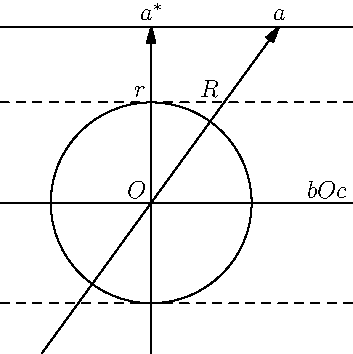
\includegraphics[width = 0.32\textwidth]{img/aabb-width-1}}%
		{\caption{原子在 $a$ 轴上的轴对齐投影}\label{fig:aabb-width-1}}
	\ffigbox[0.4\textwidth]%
		{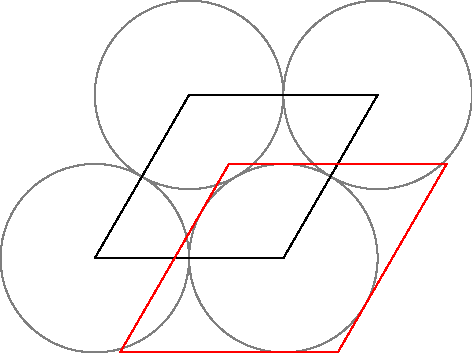
\includegraphics[width = 0.28\textwidth]{img/aabb-width-2}}%
		{\caption{一种 AABB 比晶胞大的情形}\label{fig:aabb-width-2}}
\end{floatrow}
\end{figure}

晶胞的周期边界也会影响碰撞检测,但考虑到 $T^3$ 是三维流形,流形的概念%
\parencite[161]{dodson1991}可以给我们一定的启发:可以把看成盒子的晶胞
强行分为“边界”和“内部”两部分,其内部完全类似于具有非平凡 Euclid 度规张量的
普通空间。因此,对于完全包含于晶胞内部的 AABB,可以按常规流程进行粗碰撞检测,
不用担心受周期边界的影响;而对于跨边界的 AABB,我们须要进行专门的额外检测。

\subsection{晶胞中的 sweep and prune}\label{ssec:cryst-sap}

在使用轴对齐包围盒(AABB)的碰撞检测算法中,利用树状数据结构的算法,如
\textcite{grudinin2010}的算法可以考虑已有的成键信息,因此特别适合处理成键关系
大部分已知的结构;对于成键关系总体未知的结构,我们需要的是能从头检测碰撞的算法,
而这类算法中一种最简单的是 \myterm{sweep and prune}(简称 SAP,也称为 sort and
sweep;参考 \cite[329-338]{ericson2005})。假设我们希望在非周期边界的前提下检测
$n$ 个物体(例如图 \ref{fig:sap-sweep-1} 中的那些)之间的碰撞;在 SAP 算法中,
我们会首先将物体投影到某个方便使用的坐标轴上,然后对投影区间进行碰撞检测:

\begin{figure}[htbp!]
\ffigbox%
	{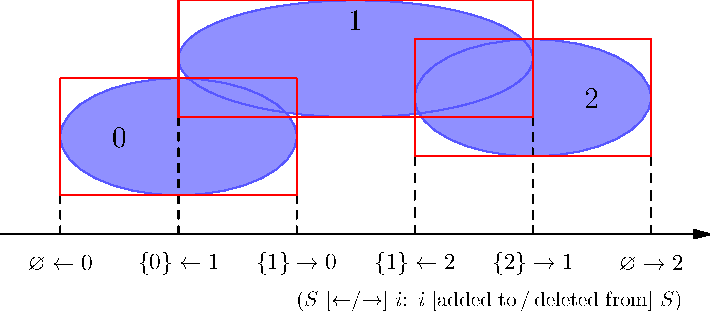
\includegraphics[width = 0.7\textwidth]{img/sap-sweep-1}}%
	{\caption{非周期边界 SAP 算法示例}\label{fig:sap-sweep-1}}
\end{figure}

\begin{itemize}
\item 将各投影区间的上下界在排序后存入一个列表 $l$(sort 步骤),
	然后建立一个空集 $S$,并通过从小到大扫描 $l$ 中的各个上下界来
	跟踪各上下界处投影区间之间的碰撞(sweep 步骤)。
\item 当扫描到一个下界时,报告相应投影区间和 $S$ 中每个区间的碰撞,
	然后将该区间插入 $S$ 中:例如在图 \ref{fig:sap-sweep-1} 中,
	当扫描到区间 \#1 的下界时,算法会先报告区间 \#0 和 \#1 之间的碰撞,
	然后将区间 \#1 插入 $S$ 中。
\item 当扫描到一个上界时,从 $S$ 中删除相应的投影区间:例如在图
	\ref{fig:sap-sweep-1} 中,当扫描到区间 \#1 的下界时,
	该区间会被从 $S$ 中删除。
\end{itemize}

在 SAP 中,$S$ 上的插入和删除操作常常并入和 SAP 的输出(报告)代码,
因此习惯上并不在粗检测的复杂度分析中考虑\parencite[333]{ericson2005}。
虽然如此,不难注意到这些操作的总复杂度取决于实际发生碰撞的物体对数:
如果每个物体都和其它所有物体发生碰撞,那么 $S$ 上的插入和删除操作无论如何
都将至少花费 $O(n^2)$ 时间。如果 sort 步骤中使用的是合适的排序算法,
例如归并排序\parencite[158-168]{knuth1998},则该步骤花费的时间在最坏的
情形下也是 $O(n\log n)$ 量级;而 sweep 步骤花费的时间显然是 $O(n)$ 量级,
所以 SAP 的总时间复杂度可以为 $O(n\log n)$ 量级。

如第 \ref{ssec:cryst-geom} 小节所述,晶胞中周期边界对粗碰撞检测算法的影响
往往可以通过对跨边界的 AABB 进行专门的额外检测来解决。就 SAP 而言,因为其
正确性依赖于每个投影区间的下界在上界之前被扫描到,周期边界所带来的问题
在于跨边界区间的上半部分在 sweep 步骤中会被算法错误地忽略:例如在图
\ref{fig:sap-sweep-2} 中,区间 \#0 的上半部分和区间 \#1 之间的碰撞就被
忽略了。然而考虑到在 sweep 步骤的末尾,集合 $S$ 中会包含所有的跨边界区间,
我们可以对常规的 SAP 算法进行如下的修改:

\begin{figure}[htbp!]
\ffigbox%
	{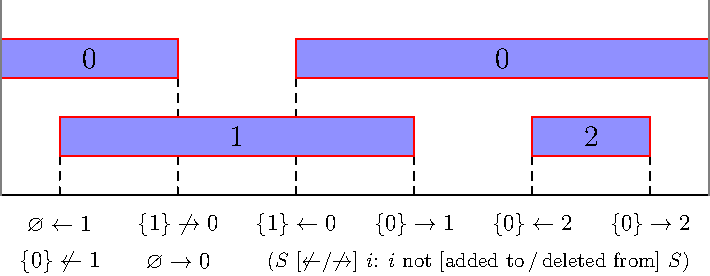
\includegraphics[width = 0.7\textwidth]{img/sap-sweep-2}}%
	{\caption{周期边界下 SAP 算法示例}\label{fig:sap-sweep-2}}
\end{figure}

\begin{itemize}
\item 执行原 SAP 算法的步骤,但当扫描到上界时须要注意,如果相应的下界尚未遇到,
	那么它们所对应的投影区间将不在集合 $S$ 中,因此试图从 $S$ 中删除相应区间
	将是无意义的。例如在图 \ref{fig:sap-sweep-2} 中,当扫描到区间 \#0 的上界时,
	我们不能从 $S$ 中删除该区间。
\item 原步骤执行完之后,再次从小到大扫描列表 $l$,但不在 $S$ 中插入区间:
	跨边界区间互相之间的碰撞在原 sweep 步骤的末尾已被处理,所以我们只关心
	不跨边界的区间和跨边界区间之间的碰撞。例如在图 \ref{fig:sap-sweep-2}
	中,再次扫描到区间 \#1 的下界时,该区间不会被插入 $S$ 中。
\item 当 $S$ 成为空集时,算法终止。例如在图 \ref{fig:sap-sweep-2} 中,
	再次扫描到区间 \#0 的上界时,算法终止。
\end{itemize}

上述改动中额外加入的新 sweep 步骤在在最坏的情形下将花费 $O(n)$ 量级的时间,
因此修改后 SAP 算法的时间复杂度仍可以为 $O(n\log n)$。在此基础之上有必要指出,
为了正确、高效地实现 SAP,一些技术细节须要特别注意:

\begin{itemize}
\item 在上述新加的 sweep 步骤中,部分碰撞对有可能会被重复报告,例如图
	\ref{fig:sap-sweep-2} 中区间 \#0 和 \#1 之间的碰撞会被报告两次,
	而这些重复的报告应该在实现时加以正确处理。
\item 上述改动通过判断投影区间的下界是否小于上界来检测跨边界区间,但这样的做法
	在区间长度不小于坐标轴的长度时(例如图 \ref{fig:aabb-width-2} 中的情形)
	会出错。为了处理这种情形,可以强行限制区间在分数坐标下的半宽最多为
	$0.5 - \varepsilon$,其中 $\varepsilon > 0$ 为一很小的常数。
\item 在 $n$ 很大的情形下,如果只在一个坐标轴上使用 SAP,碰撞对可能不会被有效
	筛除:例如在图 \ref{fig:mult-axes}(a) 中,只在 $x$ 或 $y$ 轴上使用 SAP
	都不能有效筛除碰撞对;此时在多个坐标轴上使用 SAP\footnote{%
		顺便指出,在使用多坐标轴 SAP 时正相当于构造了以物体在各坐标轴上的投影
		区间为边界的盒子,即物体的 AABB,因此 SAP 被分类为使用 AABB 的算法。%
	} 有可能会实现更高的总体性能(但也未必,参考第 \ref{ssec:cd-eval} 小节)。
\item 被检测物体在特定坐标轴上的投影区间可能特别拥挤,例如图
	\ref{fig:mult-axes}(b) 中的 $x$ 轴;此时在这些轴上使用 SAP 效果将很差,
	因此在 SAP 中可以跳过这些轴。由第 \ref{ssec:cryst-geom} 小节可知,
	在 $R/ar$ 值特别大的坐标轴上容易出现拥挤问题,
	因此在晶胞中使用 SAP 时建议不用这些轴。
\item 在物理建模中,往往可以认为一对只在彼此边界上发生碰撞的物体(例如一对
	相切的球)并不真正发生相互作用;因此如果一些上下界在 $l$ 中排名相同时,
	可以先处理上界,然后处理下界。
\item 快速排序算法\parencite[113-122]{knuth1998}在最坏情形下具有 $O(n^2)$
	的复杂度,但其平均复杂度仍为 $O(n\log n)$,且常数因子更小(参考第
	\ref{ssec:incr-intro} 小节),因此其比归并排序更适用于 SAP 中的 sort 步骤。
\end{itemize}

\begin{figure}[htbp!]\bfcmd
\ffigbox{\begin{subfloatrow}
	\setlength{\columnsep}{2em}
	\ffigbox[\FBwidth]%
		{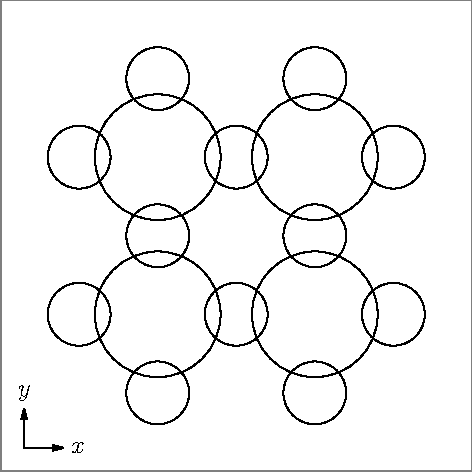
\includegraphics[height = 0.3\textwidth]{img/mult-axes-1}}%
		{\caption{一种单坐标轴 SAP 效果较差的情形}}
	\ffigbox[0.2\textwidth]%
		{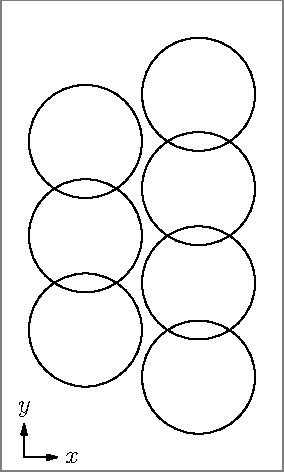
\includegraphics[height = 0.3\textwidth]{img/mult-axes-2}}%
		{\caption{一种应跳过 $x$ 轴上 SAP 的情形}}
\end{subfloatrow}}{\caption{SAP 实现中一些技术细节的示例}\label{fig:mult-axes}}
\vspace{\slop{-0.5em}}
\end{figure}

最后,考虑到因为 Coulomb 相互作用,两个原子间的正常键长可能不同于其半径之和,
我们引入\myterm{对缩放因子}(pairwise zoom factor)$p$ 的概念,其定义为
上述正常键长和半径之和的比。此外我们定义原子的\myterm{碰撞检测半径}%
(collision-detection radius)为用来计算其投影区间的半径,其等于原子的
正常半径 $r_0$ 乘以其\myterm{原子缩放因子}(atomic zoom factor)$q$。
显然,为了保证粗检测的正确性,对任意的原子对 $\{k_0, k_1\}$ 应有
\begin{equation}
	p(k_0, k_1) (r_0(k_0) + r_0(k_1)) \leq
	q(k_0) r_0(k_0) + q(k_1) r_0(k_1)\mcstop
\end{equation}

\subsection{利用等效点系对称性简化粗碰撞检测}\label{ssec:ep-sym}

因为等效点系组合法(参考第 \ref{sec:dspace-epc} 节)的使用,我们可以利用
等效点系对称性来降低晶胞粗碰撞检测的复杂度,而本节将就此进行讨论。
为了方便推导,首先约定用下标 $i$ 标记晶胞中的独立原子,其中 $i = 0, 1,
\cdots, m - 1$;用下标 $ij$ 标记独立原子 $i$ 的等效原子,其中 $j = 0, 1,
\cdots, n_i - 1$:例如在图 \ref{fig:eq-eval-1} 中,第 1 个独立原子的
第 2 个等效原子被标记为 $01$($i = 0$,$j = 1$)。考虑一个两体函数
\begin{equation}
	c(i_0j_0, i_1j_1) = c(i_1j_1, i_0j_0)\quad(i_0j_0 \neq i_1j_1)\mccomma
\end{equation}
该函数满足\myterm{等效点系对称性}:对于任何兼容于上述晶胞的对称操作 $T$,有
\begin{equation}
	c(i_0j_0, i_1j_1) = c(T(i_0j_0), T(i_1j_1))\mcscolon
\end{equation}
例如 Euclid 距离函数和第 \ref{ssec:eval-func}
小节中的对势函数(图 \ref{fig:eq-eval-2})都满足这一条件。

\begin{figure}[htbp!]\bfcmd
\setlength{\columnsep}{3em}
\begin{floatrow}
	\ffigbox[\FBwidth]%
		{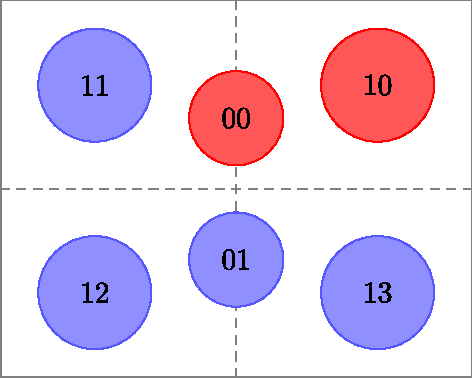
\includegraphics[width = 0.32\textwidth]{img/eq-eval-1}}%
		{\caption{等效点系对称性示例}\label{fig:eq-eval-1}}
	\ffigbox[\FBwidth]{%
		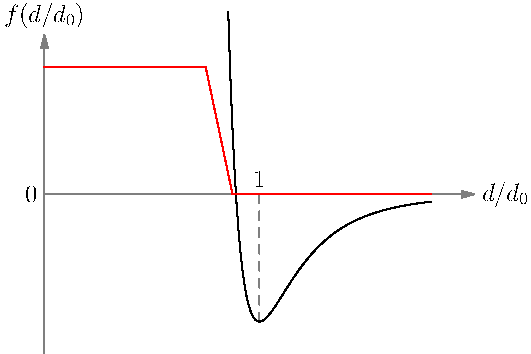
\includegraphics[width = 0.45\textwidth]{img/eq-eval-2}%
	}{%
		\captionsetup{width = 0.4\textwidth}%
		\caption[实际使用的对势和 Lennard-Jones 势的对比]%
			{实际使用的对势(浅色)和 Lennard-Jones 势(深色)的对比}%
		\label{fig:eq-eval-2}%
	}
\end{floatrow}
\end{figure}

对于任意原子 $i_0j_0$,由等效原子的定义可知必然存在一对称操作
$T_{i_0j_0}$ 将其变换为原子 $i_00$,于是有
\begin{equation}
	\sum_{i_1j_1 \neq i_0j_0}\hspace*{-1.5ex} c(i_0j_0, i_1j_1)
	= \hspace*{-1.5ex}\sum_{i_1j_1 \neq i_0j_0}\hspace*{-1.5ex}
		c(i_00, T_{i_0j_0}(i_1j_1))
	= \hspace*{-1.1ex}\sum_{i_1j_1 \neq i_00}\hspace*{-1.1ex} c(i_00, i_1j_1)
	\mccomma
\end{equation}
因此进一步有
\begin{equation}
	\sum_{\{i_0j_0, i_1j_1\}}\hspace*{-1.9ex} c(i_0j_0, i_1j_1)
	= \frac12\sum_{i_0} n_{i_0}
		\hspace*{-1.1ex}\sum_{i_1j_1 \neq i_00}\hspace*{-1.1ex} c(i_00, i_1j_1)
	= \hspace*{-1.9ex}\sum_{\{i_0j_0, i_1j_1\}}\hspace*{-1.9ex}
		\delta_{j_0} n_{i_0} c(i_0j_0, i_1j_1)\mccomma
\end{equation}
其中
\begin{equation}
	\delta_j = \left\{\,{
		\renewcommand*{\arraystretch}{0.75}
		\begin{matrix}
			1 &	(j = 0) \\
			0 &	(j \neq 0) \\
		\end{matrix}
	}\right.
\end{equation}
为 Kronecker 记号。

由此又有
\begin{equation}
	\sum_{\{i_0j_0, i_1j_1\}}\hspace*{-1.9ex} c(i_0j_0, i_1j_1)
	= \hspace*{-1.9ex}\sum_{\{i_0j_0, i_1j_1\}}\hspace*{-1.9ex} c(i_1j_1, i_0j_0)
	= \hspace*{-1.9ex}\sum_{\{i_0j_0, i_1j_1\}}\hspace*{-1.9ex}
		\delta_{j_1} n_{i_1} c(i_0j_0, i_1j_1)\mcscolon
\end{equation}
两式平均即得最终用到的关系
\begin{equation}
	C = \hspace*{-1.9ex}\sum_{\{i_0j_0, i_1j_1\}}\hspace*{-1.9ex} c(i_0j_0, i_1j_1)
	= {\textstyle\frac12} \hspace*{-1.9ex}\sum_{\{i_0j_0, i_1j_1\}}\hspace*{-1.9ex}
		(\delta_{j_0} n_{i_0} + \delta_{j_1} n_{i_1}) c(i_0j_0, i_1j_1)
	\mcstop\label{eq:ep-sym}
\end{equation}
注意如果只将不对称单元内原子的 $j$ 设为 0,则上式中
$(\delta_{j_0} n_{i_0} + \delta_{j_1} n_{i_1})$ 一项对于不对称单元外的
$\{i_0j_0, i_1j_1\}$ 对将恒为零:例如在图 \ref{fig:eq-eval-1} 中,有
\begin{equation}
	C = \frac12 \Big((2 + 4) c(00, 10) + 2c(00, \{01, 11, 12, 13\})
		+ 4c(10, \{01, 11, 12, 13\}) \Big)\mcstop
\end{equation}
由此可见其重要性:对于不对称单元外的原子对,可以不经 SAP 直接跳过细检测;
这样即使完全不使用 SAP,我们也可以将细检测的次数从 $n (n - 1) / 2$
降低到 $mn - m (m - 1) / 2$,即从 $O(n^2)$ 量级降低到 $O(mn)$ 量级。

\section{晶体学细碰撞检测}

利用第 \ref{ssec:cryst-sap}--\ref{ssec:ep-sym} 小节的算法,我们可以高效地
筛除晶胞中明显不发生碰撞或因等效点系对称性而可以跳过细碰撞检测的原子对。
本节将首先讨论晶胞中的细检测,然后构造一种评估晶胞中原子重叠状况的函数,
最后对这些算法和评估函数处理原子重叠问题的有效性和性能进行测评。

\subsection{键长计算和最邻近向量问题}\label{ssec:cryst-cvp}

在讨论晶胞中一对原子之间的“键长”时,我们指的一般是由这对原子周期性平移所得的
两套格子之间的最短距离;由平移对称性可知,后者正是由晶胞原点周期性平移所得的
格子到两原子之间位移向量的最短距离(图 \ref{fig:cryst-cvp})。由此容易注意到,
晶胞中键长的计算和\myterm{最邻近向量问题}(closest vector problem,
简称 CVP;参考 \cite{micciancio2002})之间有紧密的联系,
因为后者正是要寻找给定格子中离给定向量最近的格点。

\begin{figure}[htbp!]\bfcmd
\ffigbox%
	{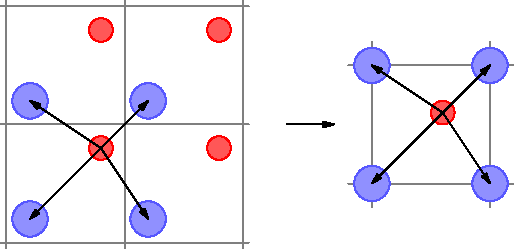
\includegraphics[width = 0.56\textwidth]{img/cryst-cvp}}%
	{\caption{键长计算和 CVP 的等价性}\label{fig:cryst-cvp}}
\end{figure}

CVP 在当代密码学研究中意义重大\footnote{%
	事实上,\emph{decryst} 这一名字除了“\textbf{de}crypt your \textbf{cryst}al
	structure”的表层含义之外,还暗示着晶体学(\textbf{cryst}allography)
	和密码学(\textbf{crypt}ography)两个领域之间因 CVP 而形成的联系。%
},在很大程度上是因为其计算复杂度随着所用向量空间的维数急剧增长,即使用量子
计算机求解也一样\parencite{micciancio2009};而如果对所用的向量空间能找到
一个尽量短且接近正交的基向量组,其计算会容易很多。晶体学中所用向量空间的
维数常常不超过 3,因此 CVP 的计算复杂度并不构成严重问题,但我们仍须进行%
\myterm{晶格归约},因为本文所用的细碰撞检测算法假定离位移向量最近的格点
一定不会在包围此向量的晶胞之外,而这意味着我们须要选取合适的晶胞
(其一反例见图 \ref{fig:bad-cell}\footnote{%
	有必要指出的是,其中按最近格点对平面进行划分得到的正是 Voronoi 图
	(参考第 \ref{ssec:narrow-discus} 小节)。%
})。

\begin{figure}[htbp!]\bfcmd
\setlength{\columnsep}{2.5em}
\begin{floatrow}
	\ffigbox[0.42\textwidth]{%
		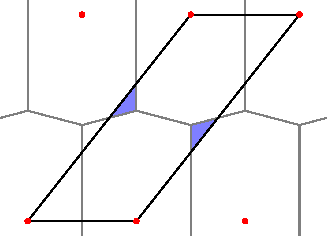
\includegraphics[width = 0.32\textwidth]{img/bad-cell}
	}{\caption[一种不好的晶胞选择]{%
		一种不好的晶胞选择,其使得离深色区域中任意点最近的格点在晶胞之外
		(浅色的分界线表示按离各个点最近的格点对平面进行的划分)%
	}\label{fig:bad-cell}}
	\ffigbox[\FBwidth]{%
		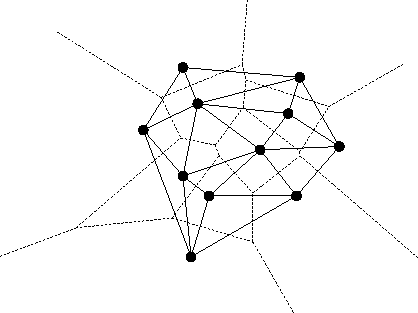
\includegraphics[width = 0.45\textwidth]{img/voro-delau}
	}{\caption[Voronoi 图和 Delaunay 三角化之间的对偶关系]{%
		Voronoi 图(虚线)和 Delaunay 三角化(实线)之间的对偶关系
		(图引自文献 (\cite[196]{berg2008}))%
	}\label{fig:voro-delau}}
\end{floatrow}
\end{figure}

在选取合适的晶胞之后便可以计算键长:首先计算两原子之间的位移向量,然后计算
包围位移向量的晶胞中所有格点和位移向量的距离里最短的一个。另一种常用算法%
\parencite{attfield1999, grudinin2010}是构造一个原子在原子对所属晶胞的所有
紧邻晶胞中的副本,然后计算这一原子以及上述所有副本到另一原子之间的距离中
最短的一个。显然,这里的算法明显快于后一种算法:对于三维晶格,
后一种算法须要计算距离 27 次,而这里的算法只需 8 次。

此外本人注意到对于分数坐标下 $l^1$ 范数
\begin{equation}
	|\upDelta x| + |\upDelta y| + |\upDelta z| < 1 / 2
\end{equation}
的位移向量,\textcite{kshirsagar2015}直接以位移向量的长度作为键长,
但本人未能找到其正确性的证明。\emph{SHELX}\parencite{sheldrick2010}%
中也采用了这一算法,但其说明中似乎未对位移向量的 $l^1$ 范数进行明确的限制。

\subsection{一种原子重叠评估函数}\label{ssec:eval-func}

如第 \ref{sec:atom-bump} 节所述,正空间法中出现原子重叠问题的原因在于 Bragg $R$
因子小的晶体模型仍可能发生原子重叠,而原始的全局最优化中也并未考虑原子重叠;
因此,如果以某种方式在最优化中考虑原子重叠,就可以自动地排除存在原子重叠的模型。
一种在全局最优化中考虑原子重叠问题的思路是修改最优化问题的约束条件,从而使得
生成的晶体模型总是那些不发生原子重叠的;然而这样会使最优化的操作变得十分繁琐,
其中最重要的原因是在上述约束条件下可行模型的集合将被分割为许多互相孤立的碎片,
这将和最优化算法中对自变量随机地进行连续微扰的做法发生冲突,
使得最优化的效率显著降低。

考虑到上述问题,本人采用了修改目标函数的做法:既然只用 $R$ 因子不能很好地排除
存在原子重叠的晶体模型,那就在目标函数中明确地加入一个对存在重叠的模型进行惩罚的
评估函数,从而使得最优化算法自动地倾向于生成无重叠的解模型。在最优化算法中,
目标函数往往被看成某种物理系统的势能函数,因此优化目标函数就是降低系统的势能;
仿照这一思路,这里的评估函数被设计为基于一个两体势
\vspace{\slop{0.3em}}
\begin{equation}
	C = \sum_{\{k_0, k_1\}} c(k_0, k_1)\mccomma\label{eq:two-body}
	\vspace{\slop{0.2em}}
\end{equation}
其中 $k$ 为晶胞中原子的编号;对势函数 $c$ 被定义为
\begin{equation}
	c(k_0, k_1) = f(d(k_0, k_1) \big/ d_0(k_0, k_1))\mccomma
\end{equation}
其中 $d$ 和 $d_0$ 分别为原子对的实际键长和正常键长。
$f$ 是一个分段线性函数,其控制节点为
\begin{equation}
	f(0) = f(0.75) = 1\mccomma f(0.875) = f(+\infty) = 0\mcscolon
\end{equation}
其形态被设计为和 Lennard-Jones 势的相似,但斜率更加平缓(图
\ref{fig:eq-eval-2})。注意到我们只在两原子间键长为正常键长的 0.875 倍时开始
考虑它们的相互作用,各原子的碰撞检测半径(参考第 \ref{ssec:cryst-sap} 小节)
可以按下式计算:
\begin{equation}
	r(k) = 0.875 q(k) r_0(k)\mcstop
\end{equation}

上述的两体势 $C$ 显然满足等效点系对称性(参考第 \ref{ssec:ep-sym} 小节),
因此可以利用 (\ref{eq:ep-sym}) 式加速计算。对于总原子数 $n$ 较大的晶胞,
因为可能有更多的原子对发生重叠,$C$ 的平均值也会比较大。为了处理这一问题,
实际算法中使用的评估函数被定义为
\begin{equation}
	B = \min(C/n, 1)\mccomma
\end{equation}
其取值上限被强行设定为 1 的原因是当 $C = n$ 时,平均每个原子会和两个原子
全面重叠,而此时可以认为相应的晶体模型是极不合理的。注意到 $B \in [0, 1]$,
如果能找到 Bragg $R$ 因子的一个上界 $\nu$,就可以将目标函数定义为
\begin{equation}
	E = \mu B + (1 - \mu) R/\nu\quad(\mu \in [0, 1])\mccomma
\end{equation}
这样对组合因子 $\mu$ 的任何值都有 $E \in [0, 1]$。事实上,
如果计算的衍射谱和实际谱都使用归一化的峰强\footnote{%
	许多从粉末衍射数据求解晶体结构的软件使用的正是归一化的峰强;本人开发的
	\emph{decryst} 也是如此,因此后者可以使用 (\ref{eq:obj-func}) 式。%
},那么可以得到
\begin{equation}
	R = \sum_i |I_{\text{obs}, i} - I_{\text{calc}, i}|
		\Big/ \sum_i I_{\text{obs}, i}
	= \sum_i |I_{\text{obs}, i} - I_{\text{calc}, i}| = 2D
	\mccomma\label{eq:total-var}
\end{equation}
其中 $D \in [0, 1]$ 为看作离散概率测度的两衍射谱之间的总变差距离%
\parencite{levin2008};于是可知 $\nu = 2$,并得到目标函数的实际公式
\begin{equation}
	E = \mu B + (1 - \mu) D = \mu B + (1 - \mu) R/2
	\mcstop\label{eq:obj-func}
\end{equation}

\subsection{原子重叠排除机制的测评}\label{ssec:cd-eval}

本小节涉及的测试代码可从 \emph{decryst} 的项目主页自由获取:%
\url{https://gitea.com/CasperVector/decryst};测试数据(含测试结构的晶胞参数、
等效点系组合和缩放因子)以及图 \ref{fig:pso-bump} 所对应的结构数据\footnote{%
	AMCSD 数据库结构代号:0005558。%
}可以从文献\parencite{liu2017}的补充材料中获取。因为 SAP 算法的常数因子较大
(从下文中可见),为了保证结果的一致性,这里只在具有最小 $R/ar$ 值(参考第
\ref{ssec:cryst-geom} 节)的单个坐标轴上使用了 SAP 算法。

为了测试第 \ref{ssec:cryst-sap}--\ref{ssec:ep-sym} 小节算法的有效性,本人从
美国矿物学家晶体结构数据库(American Mineralogist Crystal Structure Database,
简称 AMCSD;参考 \cite{downs2003})中获取了若干个不同复杂度的结构,并对每个
结构通过为独立原子赋予随机坐标的方式生成了 10000 个晶体模型。对于每个结构,
本人计算了在使用或不使用 (\ref{eq:ep-sym}) 式时(分别对应于 $N_\text{max}$
和 $N_\text{orig}$)每个模型所需细检测次数的上限,并统计了每个模型实际的细检测
次数($N_\text{real}$)和碰撞原子对数($N_\text{eff}$)的平均值和标准差,如表
\ref{tbl:cd-count} 所述。从表中可见,(\ref{eq:ep-sym}) 式和 SAP
都极大地减少了测试结构中需要细检测的原子对数。

\begin{table}[htbp!]\bfcmd
\ttabbox[0.75\textwidth]{\begin{tabular}{
	crrrrS@{\extracolsep{0.75em}}S
}\toprule
	ID &	$n$ &	$m$ &	$N_\text{orig}$ & $N_\text{max}$ &
	{$N_\text{real}$} &	{$N_\text{eff}$} \\\midrule
	0005558 &	24 &	5 &	276 &	105 &	50(3) &	8(3) \\
	0015840 &	64 &	8 &	2016 &	476 &	212(8) &	10(4) \\
	0009272 &	64 &	8 &	2016 &	476 &	218(24) &	43(22) \\
	0009563 &	90 &	10 &	4005 &	845 &	350(22) &	23(8) \\
	0002630 &	126 &	14 &	7875 &	1659 &	550(9) &	29(8) \\
	0000427 &	152 &	20 &	11476 &	2830 &	581(32) &	40(9) \\
	0000447 &	160 &	4 &	12720 &	630 &	227(11) &	8(3) \\\bottomrule
\end{tabular}}{\caption[碰撞检测算法的有效性测评]{%
	碰撞检测算法的有效性测评:ID 为测试结构在 AMCSD 中的代号;$n$ 和 $m$ 分别为
	晶胞中的总原子数和独立原子数;$N_\text{max}$ 和 $N_\text{orig}$ 分别为每个
	模型在用或不用 (\ref{eq:ep-sym}) 式时所需的细检测次数;$N_\text{real}$ 和
	$N_\text{eff}$ 分别为每个模型实际的细检测次数和碰撞原子对数。%
}\label{tbl:cd-count}}
\end{table}

为了测试上文中算法的性能,对于上述的每个测试结构,本人在不同条件下执行了一个测试
程序,每个条件下测试了 250 组晶体模型,每组由 250 个通过为独立原子赋予随机坐标
的方式生成的模型构成:
\begin{itemize}
	\item ($t_\text{void}$)不进行任何碰撞检测,只生成随机的晶体模型;
		该条件下度量的是测试程序本身的时间开销。
	\item ($t_\text{bn}$)无 SAP,只使用 (\ref{eq:ep-sym}) 式筛选原子对,
		细检测步骤被设为空指令;该条件下度量的是只使用 (\ref{eq:ep-sym})
		式进行粗检测的时间开销。
	\item ($t_\text{bN}$)无 SAP,只使用 (\ref{eq:ep-sym}) 式筛选原子对,
		但正常执行细检测步骤;该条件下度量的是只使用 (\ref{eq:ep-sym})
		式进行完整碰撞检测的时间开销。
	\item ($t_\text{Bn}$)使用 (\ref{eq:ep-sym}) 式和 SAP 筛选原子对,
		但细检测步骤被设为空指令;该条件下度量的是同时使用
		(\ref{eq:ep-sym}) 式和 SAP 进行粗检测的时间开销。
	\item ($t_\text{BN}$)完全的碰撞检测;该条件下度量的是使用
		(\ref{eq:ep-sym}) 式和 SAP 进行完整碰撞检测的时间开销。
	\item ($t_\text{orig}$)不使用 (\ref{eq:ep-sym}) 式或 SAP,
		但正常执行细检测步骤;该条件下度量的是逐对算法的时间开销。
\end{itemize}

对以上每种条件,本人在 Intel i7-3720QM CPU 上收集了测试程序在每组模型上所花费
时间的平均数和标准差,并将其除以每组的模型数,结果如表 \ref{tbl:cd-time} 所述。
从表中可见,对于各个复杂度的测试结构,第 \ref{ssec:cryst-sap}--\ref{ssec:ep-sym}
小节的算法都极大地降低了碰撞检测所花费的总时间;而且随着晶胞中原子数的增加,
这些算法和逐对算法相比的优势体现得更加显著。有必要强调的是,从表中也可以注意到,
虽然 SAP 是 $O(n\log n)$ 的算法,但是其常数因子较大(参考第 \ref{ssec:cryst-sap}
小节中归并排序和快速排序的比较),因此对于较小的晶胞而言只使用 (\ref{eq:ep-sym})
式进行粗检测可能在性能上会更有利。

\begin{table}[htbp!]\bfcmd
\sisetup{table-number-alignment = center}
\ttabbox{\begin{tabular}{
	cS[table-format = 1.5]@{\extracolsep{0.5em}}
	S[table-format = 2.5]@{\extracolsep{0.5em}}
	S[table-format = 3.4]@{\extracolsep{0.5em}}
	S[table-number-alignment = center-decimal-marker]@{\extracolsep{0.75em}}
	S[table-number-alignment = center-decimal-marker]@{\extracolsep{0.75em}}
	S[table-number-alignment = center-decimal-marker]
}\toprule
	ID &	{$t_\text{void}$} &	{$t_\text{bn}$} &	{$t_\text{bN}$} &
	{$t_\text{Bn}$} &	{$t_\text{BN}$} &	{$t_\text{orig}$} \\\midrule
	0005558 &	0.88(7) &	1.19(7) &	7.4(2) &
	8.0(2) &	10.9(3) &	17.6(5) \\
	0015840 &	1.8(1) &	3.2(1) &	31.8(8) &
	30.6(7) &	44(1) &	135(2) \\
	0009272 &	2.3(2) &	3.6(1) & 	31.4(4) &
	34.3(6) &	47(2) &	130(2) \\
	0009563 &	2.76(7) &	5.2(2) &	54.0(8) &
	57.3(6) &	78(1) &	257(3) \\
	0002630 &	3.6(1) &	8.0(2) &	105(1) &
	90(1) &	121(1) &	496(5) \\
	0000427 &	4.2(1) &	12(1) &	180(6) &
	91(2) &	124(3) &	727(7) \\
	0000447 &	3.8(1) &	5.6(2) &	46.2(6) &
	83(2) &	98(2) &	886(11) \\\bottomrule
\end{tabular}}{\caption[碰撞检测算法的性能测评]{%
	测试程序在每个模型上花费的时间(\si{\micro\second})。
	$t_\text{void}$:只生成模型;
	$t_\text{bn}$:使用 (\ref{eq:ep-sym}) 式;
	$t_\text{bN}$:(\ref{eq:ep-sym}) 式和细检测;
	$t_\text{Bn}$:(\ref{eq:ep-sym}) 式和 SAP;
	$t_\text{BN}$:(\ref{eq:ep-sym}) 式、SAP 和细检测;
	$t_\text{orig}$:使用逐对算法。%
}\label{tbl:cd-time}}
\end{table}

为了测试第 \ref{ssec:eval-func} 小节中原子重叠评估函数的有效性,本人利用
同一小节中的目标函数 $E$ 对 \ce{PbSO4} 结构进行了求解:对于组合因子
$\mu = 0, 0.01, 0.02, \cdots, 0.5$ 的每个值\footnote{%
	上限取 0.5 是考虑到我们的最终目标是结构测定。%
},本人利用全局最优化算法生成了 1000 个随机的解模型,
并统计了它们的 $(D, B)$ 分布,如图 \ref{fig:db-distrib-1} 所示。
由图可见正确解的 $D = R/2$ 值并不是最低的,而 $D$ 值最低的解中都有严重的
原子重叠问题,这正好解释了第 \ref{sec:atom-bump} 节提到的通过最小化
$R$ 因子求解 \ce{PbSO4} 结构得到的多数是错误解的现象。

\begin{figure}[htbp!]\bfcmd
\ffigbox{%
	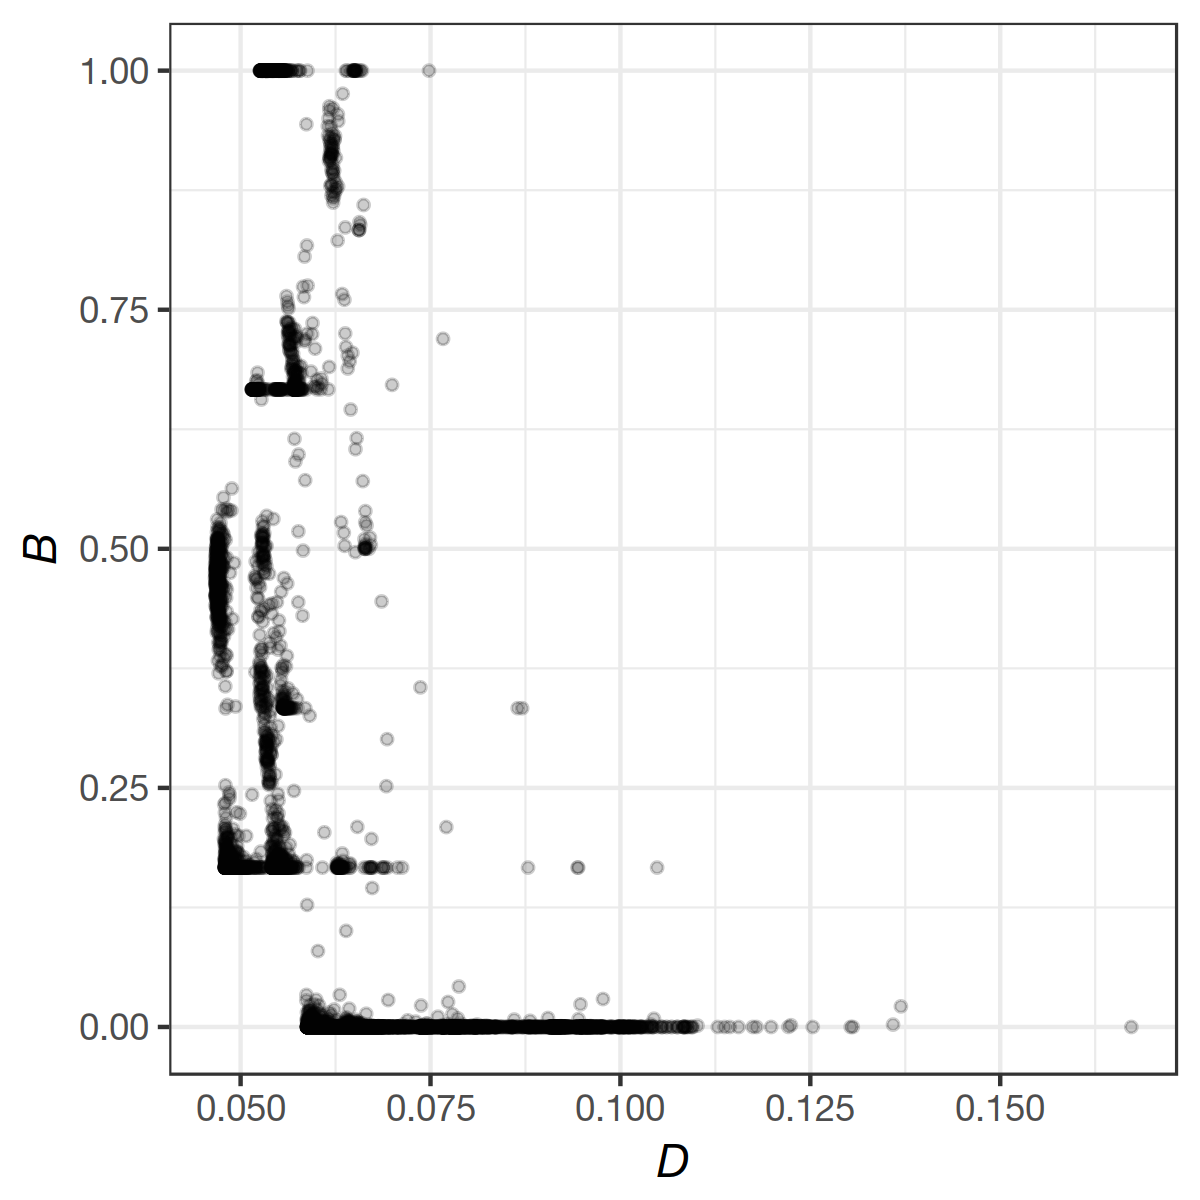
\includegraphics[width = 0.6\textwidth]{img/db-distrib-1}%
}{\caption[\ce{PbSO4} 随机解模型的 $(D, B)$ 分布]{%
	$\mu = 0, 0.01, 0.02, \cdots, 0.5$,每个 $\mu$
	值所对应 1000 个解模型的总体 $(D, B)$ 分布%
}\label{fig:db-distrib-1}}
\end{figure}

考虑到 $D$ 和 $B$ 都是原子坐标的连续函数,且两者都在和晶胞兼容的对称操作
之下保持不变,因为正确解的 $D = R/2 = 0.0642$、$B = 0$,
根据上图可以假定所有正确\footnote{%
	所有由对称操作所联系的模型都视为同一模型,
	而只在原子坐标上有细微差别的模型也视为等价。%
}的解模型都满足 $D < 0.12$、$B < 0.05$。为了
验证这一判据,本人生成了 100 个随机的满足判据的解模型,其中 $\mu \in [0, 0.5]$
为随机选取;在人工检查每个解之后,可以发现其中 99 个是正确的,而唯一错误解(图
\ref{fig:verify-fail})的 $D = 0.0814$(所有 100 个解中最大,次大值为 0.0705)。
本人由此假定一个解正确的充分必要条件为其 $D < 0.075$、$B < 0.05$,并统计了每个
$\mu$ 值所对应 1000 个解中正确解的比例,如图 \ref{fig:db-distrib-2} 所示。由图
可见,上述的评估函数在最优化的过程中有效地排除了 \ce{PbSO4} 的不合理晶体模型。

\begin{figure}[htbp!]\bfcmd
\vspace{\slop{0.3em}}
\setlength{\columnsep}{3em}
\begin{floatrow}
	\ffigbox[0.33\textwidth]{%
		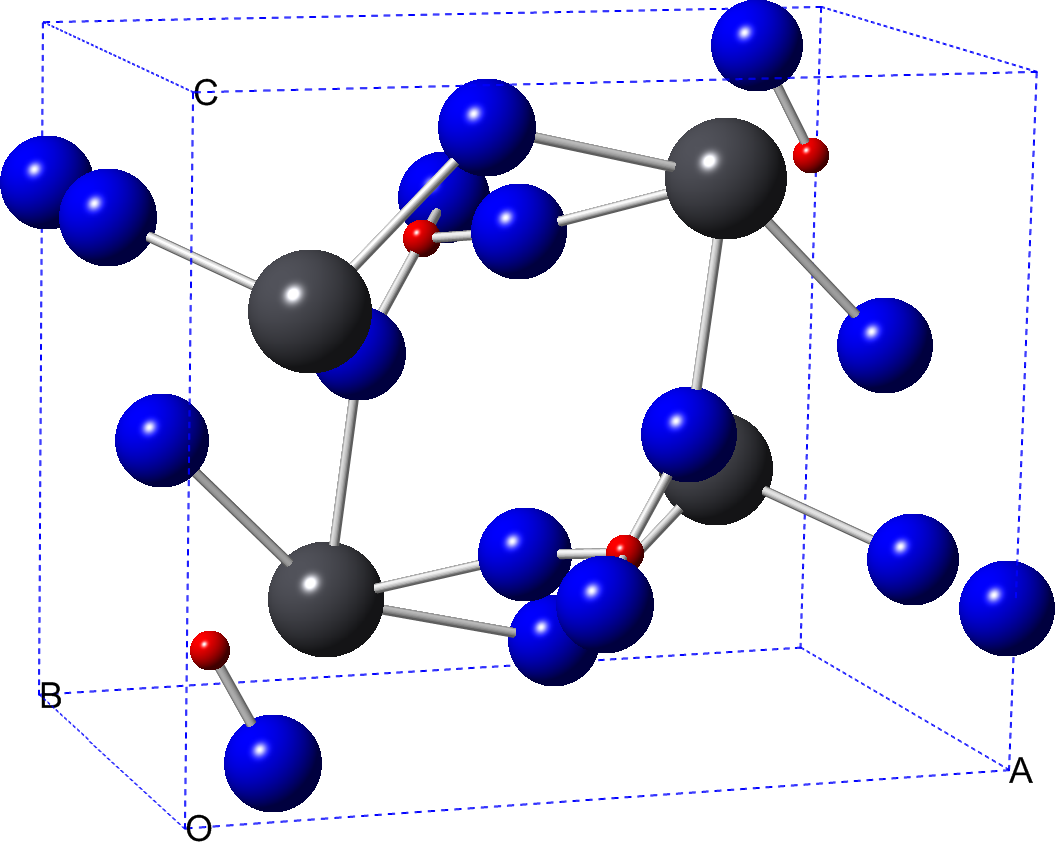
\includegraphics[width = 0.3\textwidth]{img/verify-fail-1}
	}{\caption[一个指标几乎合理的错误解]{%
		一个指标几乎合理的错误解($D = 0.0814$,$B = 0$)
	}\label{fig:verify-fail}}
	\ffigbox[\FBwidth]%
		{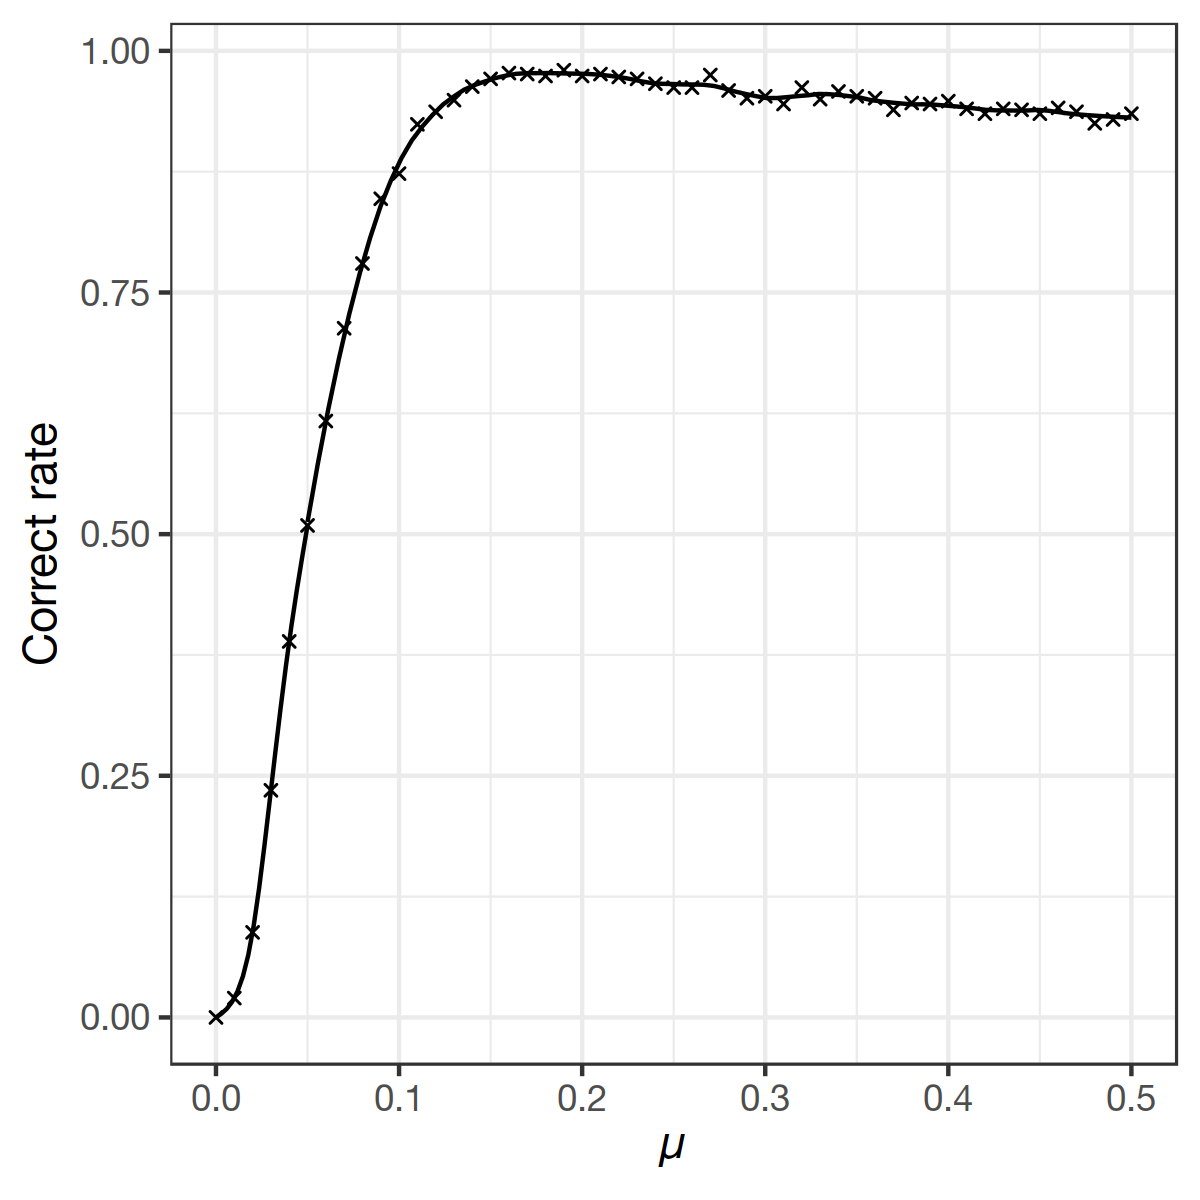
\includegraphics[width = 0.5\textwidth]{img/db-distrib-2}}%
		{\caption{不同 $\mu$ 值所对应解的实验正确率}\label{fig:db-distrib-2}}
\end{floatrow}
\vspace{\slop{-0.3em}}
\end{figure}

\section{讨论和小结}
\subsection{关于细碰撞检测正确性的讨论}\label{ssec:narrow-discus}

如第 \ref{ssec:cryst-cvp} 小节所述,本文中计算键长的算法假定已经选取合适的
晶胞,从而使得离位移向量最近的格点一定不会在包围此向量的晶胞之外。然而,能这样
做的条件是对每一个晶格都至少存在一个满足要求的晶胞,但本人未能找到这一条件的
严格证明。希望理论工作者能证明或证伪这一条件,并(如果条件是正确的)给出一种构造
合适晶胞的算法;另一方面,如果这一条件是错误的,本文中的细检测算法将不得不搜索
更多的近邻晶胞以寻找离位移向量最近的格点,但本文中的粗检测算法将不需改动。

考虑到在二维情形下,晶胞出现类似于图 \ref{fig:bad-cell} 中问题的前提是其一对对边
在正交投影下没有重叠(图 \ref{fig:voro-trans}),而晶格归约中的 Seeber 算法%
\parencite{engel1986}正好会排除这种情形,后者可能会在上述问题的研究中
有一定的启发意义。另一种或许具有可行性的研究思路是利用 Voronoi 图%
\parencite[147-171]{berg2008}和 Delaunay 三角化\parencite[191-218]{berg2008}%
之间的对偶关系(图 \ref{fig:voro-delau}):本人猜想,格点的 Delaunay 三角化%
\parencite{caroli2016}可能满足离任意点最近的格点是其一包围单纯形的顶点;
在此基础之上,通过适当拼接这些单纯形,或许就可以得到满足要求的晶胞。
此外在二维情形下,Delaunay 三角化会最小化所有三角形中的最大内角,
而这似乎也和晶格归约有一定的内在关联。

\begin{figure}[htbp!]\bfcmd
\ffigbox%
	{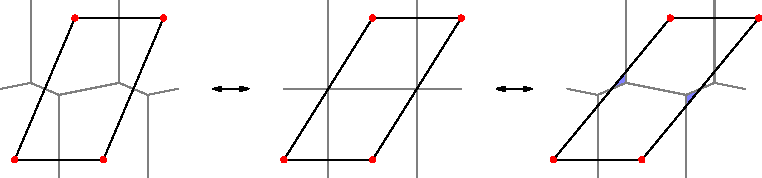
\includegraphics[width = 0.96\textwidth]{img/voro-trans}}%
	{\caption{格点的 Voronoi 图随晶胞参数的变化}\label{fig:voro-trans}}
\end{figure}

最后有必要指出,如果第 \ref{ssec:cryst-cvp} 小节中对 $l^1$ 范数小于 $1/2$
的位移向量计算键长的简便算法被证明是正确的,那么我们将能大幅度地进一步减少
计算短距离原子对键长所花费的时间。尽管上述简便算法尚无严格证明,但本人倾向于
认为其是正确的,只是需要一定的限制条件,包括合适的晶胞选择\footnote{%
	本人在某些限制条件下对随机产生的晶胞进行了测试(具体代码参考第
	\ref{ssec:decr-arch} 小节中的说明),未能找到这一简便算法的反例。
	随机测试显然不能取代严格证明,但本人基于此测试猜想这一算法应该正确。%
}(例如图 \ref{fig:bad-cell} 中的晶胞便会使上述简便算法出错)。另外,如果在某些
应用场景下,对于原子对没有进行除了 (\ref{eq:ep-sym}) 式之外的筛选,那么长距离原
子对将不能被充分筛除,因此在这些应用场景中上述算法带来的性能提升将较为有限。

\subsection{其它讨论}

(\ref{eq:ep-sym}) 式并未彻底利用特殊位置的对称性:例如在图 \ref{fig:eq-eval-1}
中因为 $c(00, 10) = c(00, 11)$、$c(00, 12) = c(00, 13)$,
总的两体势事实上可以被进一步归约为
\begin{equation}
	C = c(00, 01) + 4c(00, 10) + 2c(00, 12) + 2c(10, \{01, 11, 12, 13\})\mcstop
\end{equation}
如果这样的归约能自动进行,那么 $C$ 的计算将能进一步简化;然而这样很可能将需要一
个比 (\ref{eq:ep-sym}) 式中的 $(\delta_{j_0}n_{i_0} + \delta_{j_1}n_{i_1}) / 2$
复杂得多的原子对多重度计算公式,而后者本身的计算开销未必能被其对
$C$ 的简化所带来的性能提升所补偿。

在表 \ref{tbl:cd-time} 中,尽管“0000447”是总原子数 $n$ 最大的结构,
但其 $t_\text{bN}$ 却小于 $t_\text{BN}$,这是因为其独立原子数 $m$ 太小,
导致其晶体模型中绝大多数原子对被 (\ref{eq:ep-sym}) 式筛除。此外尽管如第
\ref{ssec:cryst-sap} 小节所述,SAP 算法并不特别适用于成键关系大部分已知的结构,
但如果这类结构中的成键信息因故不须在碰撞检测中考虑时,其也可以用 SAP 来处理:在
表 \ref{tbl:cd-time} 中,“0015840”(其中唯一的分子晶体)的测试结果和“0009272”
的结果相差并不大,这在两结构的 $n$、$m$ 值都完全相同的背景之下不难理解。

更加复杂的两体势,例如 \textcite{bushmarinov2012}所用的势或者甚至吸引势,原则上
也是可以在实际的评估函数中使用的。第 \ref{ssec:eval-func} 小节中的对势 $c$ 只
仿照了 Lennard-Jones 势中的排斥部分,因为本人认为我们的目标是排除原子重叠,而
不是对原子之间的相互作用进行精确的建模。虽然如此,从第 \ref{ssec:cd-eval} 小节
可见,目前使用的评估函数应该至少对包括 \ce{PbSO4} 在内的一些简单结构是有效的,
而其在求解更复杂结构时的应用将在第 \ref{chap:decr-usage} 章中展示。

对于很复杂的结构,特别是独立原子数很大的结构,期望只使用 Bragg $R$ 因子和原子
重叠评估函数就能成功求解是不太现实的:在这些结构的晶体模型中,完全有可能存在一些
$R$ 因子合理且无明显原子重叠,但在成键类型、配位数、配位多面体形态、键价等等
方面有问题的模型。相应地,我们须要在结构测定中应用更多的\myterm{结构验证}%
(structure validation;参考 \cite{spek2003})手段,而第 \ref{chap:decr-usage}
章将给出一些通过人工方式进行结构验证的例子;但为了实现使结构测定更加自动化的
目标,我们最终须要做的显然是将更多的结构验证技术自动化地引入结构测定中。考虑到在
结构验证中很多测试都以结构中的成键关系为基础,可以认为第 \ref{ssec:cryst-sap}--%
\ref{ssec:ep-sym} 小节的算法应该会在这些方面的研究中发挥基础性的作用。

\subsection{本章小结}

针对晶体结构测定中的原子重叠问题,本人基于轴对齐包围盒(AABB)模型提出了
一种具有通用性的晶体学碰撞检测算法框架。为了处理成键关系总体未知的结构,
本人基于上述框架修改了 sweep and prune(SAP)算法,使之能以 $O(n\log n)$
的时间复杂度检测晶胞中的成键关系。考虑到在求解成键关系总体未知的结构时常常
使用等效点系组合(EPC)法,本人也提出了一种利用等效点系对称性极大降低碰撞
检测复杂度的算法,这一算法即使对于小晶胞也可以显著降低碰撞检测的时间开销。
基于以上算法,本人提出了一种针对晶胞中原子重叠状况的评估函数,其可以用于
在正空间法的全局最优化步骤中实时地排除存在原子重叠的晶体模型;此外,
上述算法对于晶胞中配位多面体、原子键价等等的计算也具有重要的意义。

\begin{rquote}{}
	即得易见平凡,仿照上例显然;留作习题答案略,读者自证不难。\\
	反之亦然同理,推论自然成立;略去过程 Q.E.D.,由上可知证毕。
\end{rquote}
\rightline{——《\emph{西江月·证明}》(摘自互联网)}

% vim:ts=4:sw=4

	% Copyright (c) 2014,2016,2018 Casper Ti. Vector
% Public domain.

\chapter{\emph{decryst}:高效的粉晶结构测定软件}\label{chap:decr-theory}
\section{\emph{decryst} 中的增量计算}\label{sec:decr-incr}

如第 \ref{sec:atom-bump} 节所述,针对成键关系总体未知的结构,为了提升排除原子
重叠的效率,本人基于第 \ref{chap:cryst-cd} 章中的机制开发了 \emph{decryst}。
本人在开发 \emph{decryst} 的过程中,通过应用增量计算的思想,使其全局最优化
步骤的性能得到了大幅度的提升(参考第 \ref{ssec:incr-obj} 小节);除此之外,
通过增量生成等效点系组合,本人极大地降低了 \emph{decryst} 的内存需求(参考第
\ref{ssec:incr-epc} 小节)。此外,在讨论这些问题之前,第 \ref{ssec:incr-intro}
小节将简要回顾 \emph{decryst} 中应用的和增量计算相关的技术。

\subsection{增量计算和惰性计算}\label{ssec:incr-intro}

\myterm{增量计算}的思想在计算机科学技术的发展中有着深远的影响:于 70 年代
后期出现在 Unix 中的 \verb|make| 程序\parencite{feldman1979}会检测软件
项目中发生变更的模块,然后执行命令根据依赖关系重新构建所有受影响的模块(图
\ref{fig:make-build}),从而避免重复构建未发生变更的模块;于 2016 年推出的视频
游戏 \emph{Doom} 中,通过在渲染每一帧画面时巧妙地利用为前一帧画面计算的数据,制
作方将游戏的画面品质和图形性能提升到了新的水平\parencite{correges2016}。有必要
指出,增量计算和\myterm{惰性计算}是一脉相承的,因为合理地避免多余的计算可以说
正是惰性计算的核心思想;受此启发,在 \emph{decryst} 中,除了增量计算之外,本人
也应用了其它的可归类为惰性计算的技术,而本小节将对这些技术进行简短的总结。

\begin{figure}[htbp!]\bfcmd
\ffigbox{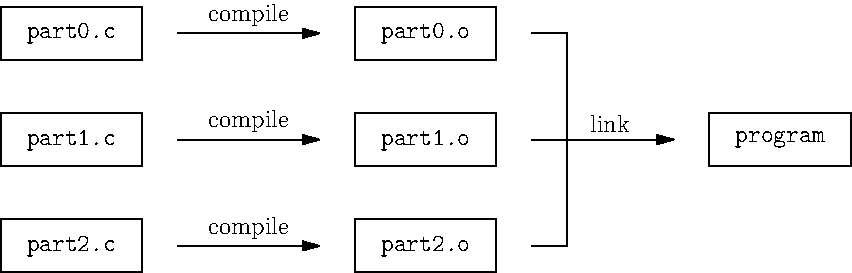
\includegraphics[width = 0.64\textwidth]{img/make-build}}{\caption[%
	\texttt{make} 如何构建一个示例程序%
]{%
	\texttt{make} 如何构建一个示例程序:在 \texttt{program} 构建完成之后,
	如果 \texttt{part0.c} 发生变更,为了再次构建 \texttt{program},\texttt{make}
	只须重新编译 \texttt{part0.c} 然后重新链接所有 \texttt{.o} 文件%
}\label{fig:make-build}}
\end{figure}

首先,本人认为代码中处理对象的分离(separation of concerns)和惰性计算的思想是
符合的:例如全局最优化的代码不应该关心结构中所涉及化学元素的名称和符号,更不应该
关心在绘制结构图时使用什么颜色的球体来表示其中的原子。通过对各模块所处理对象的
细致分离,我们不仅会使软件的架构更加清晰,也会减少各模块代码所从事的无用工作,
因此在增强软件可维护性的同时也提升了软件的性能。在 \emph{decryst} 的架构设计中,
这一原则的一些具体体现可以参考第 \ref{ssec:decr-arch} 小节。

其次,CPU 缓存\parencite{bryant2011}可以认为是一种通过硬件实现的惰性计算技术,
这一技术使得对连续内存区域的访问被定向到访问效率远快于内存的缓存,从而提升程序
性能。相应地,利用 CPU 缓存的方法是使用对缓存友好的算法和数据结构,从而尽量
利用连续的内存区域:例如在可行的前提下,尽量使用快速排序算法而非归并排序算法
(参考第 \ref{ssec:cryst-sap} 小节),使用数组而非链表,等等。

根据增量计算避免重新计算未改变值的思想,对于值不发生改变的函数,在首次求值
之后便不须重新求值了;而如果将这些函数的求值提前到程序的开头,我们所做的
就是建立查找表。对于计算开销很大的函数,使用查找表显然十分有利:
例如在正空间法的全局最优化步骤中,对于 X 射线原子散射因子
\begin{equation}
	f_\mathrm{X}(hkl) = g_\mathrm{X}(\sin\theta_{hkl} / \lambda)
	= c_\mathrm{X} + \sum_i a_{\mathrm{X},i} \iee ^
		{b_{\mathrm{X},i} (\sin\theta_{hkl} / \lambda) ^ 2}\mccomma
\end{equation}
注意到其求值须要多次用到计算较慢的指数函数和正弦函数,其计算开销显然很大;
又因为其值只取决于衍射指标 $hkl$、元素 X 和在最优化步骤中不变的波长
$\lambda$,所以其特别适合使用查找表。因为上述原因,\emph{decryst}
会在最优化程序的一开始建立包括原子散射因子在内若干函数的查找表。

\emph{decryst} 使用模拟退火作为其全局最优化算法,而后者可以和物理退火相类比:
既然保温可以让系统趋于平衡,如果在系统始终不太远离平衡的前提下逐渐降低温度,就
可以期望使系统接近低温下的平衡态。显然,如果系统已经很接近平衡,就不必再保温,
这样可以减少非必要的保温过程所花费的时间,而这正是自适应模拟退火的思路:不是在
每个温度阶梯上保温固定的时间,而是在检测到系统接近平衡时自动降温。就目前而言,%
\emph{decryst} 在其最优化步骤中使用的是 \textcite{lam1988}的自适应模拟退火
算法,因为对后者可以比较方便地进行并行化(参考第 \ref{ssec:decr-para} 小节)。

最后,注意到晶胞中常有的对称性,以及结构因子的计算开销在全局最优化总开销
中的高权重(参考第 \ref{ssec:incr-obj} 小节),\emph{decryst} 中也利用
以下关系来降低结构因子的计算开销(其中 $\vec{q}$ 为散射向量):
\begin{equation}
	F_\text{反演对称}(\vec{q}) = \sum_i f_i(\vec{q}) (
		\iee ^ {2\uppi\eye\vec{q} \cdot \vec{x}_i} +
		\iee ^ {2\uppi\eye\vec{q} \cdot (-\vec{x}_i)}
	) = 2\sum_i f_i(\vec{q}) \cos(2\uppi\vec{q} \cdot \vec{x}_i)
	\mccomma\label{eq:cent-sym}
\end{equation}
其中 $i$ 为中心对称原子对的编号;
\begin{equation}
	F_\text{带心格子}(\vec{q}) = \sum_{ij} f_i(\vec{q})
		\iee ^ {2\uppi\eye\vec{q} \cdot (\vec{x}_i + \vec{r}_j)}
	= \sum_i f_i(\vec{q}) \iee ^ {2\uppi\eye\vec{q} \cdot \vec{x}_i}
		\sum_j \iee ^ {2\uppi\eye\vec{q} \cdot \vec{r}_j}\mccomma
\end{equation}
其中 $\vec{r}_j$ 为可选原点的坐标。

最后有必要指出,惰性计算技术或多或少地在其它晶体学软件中有所应用,而且其对软件
性能的影响是较为显而易见的,但本人未能找到一个较为全面的对以上技术的总结。这样的
现状所造成的一个不良的结果是部分晶体学软件对这些技术的忽视,例如 \emph{EPCryst}%
\parencite{deng2011}在上述技术中只应用了查找表这一项技术,这使得其在 \ce{PbSO4}
正确等效点系组合的全局最优化中比 \emph{decryst} 慢了两个数量级\footnote{%
	根据本人的测试,在 Intel i7-3720QM CPU 上,\emph{EPCryst}
	耗时多于 \SI{1000}{\second},而 \emph{decryst}
	即使在不用增量计算的前提下耗时也少于 \SI{10}{\second}。%
}。
正因如此,本人希望本小节中的总结能对晶体学软件的设计者有所帮助。

\subsection{目标函数的增量计算}\label{ssec:incr-obj}

因为 \emph{decryst} 使用 (\ref{eq:obj-func}) 式中的函数 $E$ 作为全局最优化的目标
函数(参考第 \ref{ssec:eval-func} 小节),为了加速最优化,我们事实上须要加速
Bragg $R$ 因子和原子重叠评估函数 $B$ 的计算;又因为计算 $R$ 因子时大部分时间
用在计算结构因子上,我们显然须要加速结构因子的计算。考虑到两个相邻的最优化循环中
晶体模型之间的差别只在于某一个独立原子位置的移动,根据 Fourier 变换的可加性有
\begin{equation}
	F'(\vec{q}) - F(\vec{q}) = \sum_i f_i(\vec{q}) (
		\iee ^ {2\uppi\eye\vec{q} \cdot \vec{x}'_i}
		- \iee ^ {2\uppi\eye\vec{q} \cdot \vec{x}_i}
	)\mccomma
\end{equation}
其中 $i$ 是被移动原子的编号。根据这一关系,我们可以利用前一晶体模型的结构因子
数据增量地计算后一晶体模型的结构因子:只须对被移动的原子重新计算 $\iee ^
{2\uppi\eye\vec{q} \cdot \vec{x}_i}$ 项的值即可。由此可知,如果晶胞中有 $m$
个独立原子,而这些原子在各最优化循环中被轮流移动,那么晶胞中所有原子结构因子的
重新计算将被 $m$ 个最优化循环分担(而非原先的在单个最优化循环中完成),于是结构
因子的计算性能将是原先算法的 $m$ 倍。

类似地,对于 $B$ 所依赖的两体势 $C$(参考 \ref{eq:two-body} 式),显然其中对势
函数 $c(k_0, k_1)$ 的值只在 $\{k_0, k_1\}$ 对中至少一个原子被移动时发生改变;
因此 $C$ 的值也可以增量地计算,只须对上述原子对重新进行碰撞检测和处理即可。又注
意到利用等效点系对称性(参考第 \ref{ssec:ep-sym} 小节),我们只须对含独立原子的
原子对进行碰撞检测,所以最终细碰撞检测次数的上限是 $(n - 1) + (m - 1)(n' - 1)$,
其中 $n$、$m$、$n'$ 分别为晶胞的总内原子数、独立原子数和被移动独立原子的等效
原子数。在平均意义下,上述碰撞检测的时间复杂度是 $O(n)$ 量级,因此我们不再须要
专门使用类似于 sweep and prune(参考第 \ref{ssec:cryst-sap} 小节)的粗碰撞检测
算法以避免逐对碰撞检测的 $O(n^2)$ 复杂度,这在上述 SAP 算法常数因子较大的背景
之下尤其值得注意;相应地,因为不再须要计算原子的投影区间,我们也就不再须要使用
原子缩放因子,而是只需要对缩放因子。此外有必要特别提请注意的是,当最优化
循环的次数很大时,增量求和的浮点数误差积累可能会造成严重的问题,而类似于
\textcite{kahan1965}算法的增量浮点数求和算法难以应用,因为被求和数的
平均值渐进地趋于零\parencite{higham1993}。就目前而言,\emph{decryst}
通过在增量求和中使用定点数来绕过这一问题,因为定点数算术是没有误差的。

最后,本人在 Intel i7-3720QM CPU 上就增量计算对全局最优化步骤性能的影响
进行了测评。除了可以从项目主页 \url{https://gitea.com/CasperVector/decryst}
获取的数据之外,其它测试数据可以从文献\parencite{liu2018}的补充材料中获取。
本人从 AMCSD 数据库\parencite{downs2003}中获取了若干个不同复杂度的结构,
并对这些结构计算了目标函数:具体而言,对于每一个测试结构,本人测试了 100 组
晶体模型,每组由 100 个通过为独立原子赋予随机坐标的方式生成的模型构成。
本人度量了在使用或不使用增量计算(分别对应于 $t_{\cdots,\text{incr}}$ 和
$t_{\cdots,\text{orig}}$)时对每组模型计算整个目标函数 $E$ 或只是 Bragg $R$
因子所花费时间(分别对应于 $t_{E,\cdots}$ 和 $t_{R,\cdots}$)的平均值和
标准差,并将其除以每组的模型数,结果如表 \ref{tbl:incr-eval} 所述。

\begin{table}[htbp]\bfcmd
\sisetup{table-number-alignment = center}
\ttabbox{\begin{tabular}{
	crrr@{\extracolsep{1.5em}}
	S[table-format = 2.4]@{\extracolsep{1em}}
	S[table-number-alignment = center-decimal-marker]@{\extracolsep{1.25em}}
	S[table-format = 2.4]@{\extracolsep{1.25em}}
	S[table-number-alignment = center-decimal-marker]
}\toprule
ID &	$n$ &	$m$ &	$N_\text{refl}$ &	{$t_{R,\text{incr}}$} &
{$t_{R,\text{orig}}$} &	{$t_{E,\text{incr}}$} &	{$t_{E,\text{orig}}$} \\\midrule
0005558 &	24& 5& 94 &	8.9(3) &	43.9(5) &	12.5(7) &	44.5(7) \\
0009272 &	64& 8& 80 &	39.7(9) &	241(3) &	50.6(6) &	242(3) \\
0009563 &	90& 10& 76 &	15.0(2) &	168(3) &	30.0(7) &	174(2) \\
0002630 &	126& 14& 73 &	11.3(3) &	244(3) &	30.7(3) &	252(2) \\
0000427 &	152& 20& 374 &	27.4(5) &	639(7) &	53.6(7) &	663(8) \\
0000447 &	160& 4& 32 &	27.0(9) &	87(2) &	59(1) &	102(2) \\\bottomrule
\end{tabular}}{\caption[\emph{decryst} 中增量计算的性能测评]{%
	\emph{decryst} 中增量计算的性能测评(时间单位为 \si{\micro\second}):ID
	为测试结构在 AMCSD 中的代号,$n$ 和 $m$ 分别为晶胞中的总原子数和独立原子
	数,$N_\text{refl}$ 为有记录的衍射峰数;$t_{E,\cdots}$ 和 $t_{R,\cdots}$
	分别为计算每个模型 $E$、$R$ 所需的时间; $t_{\cdots,\text{incr}}$ 和
	$t_{\cdots,\text{orig}}$ 分别为用或不用增量计算时所需的时间。%
}\label{tbl:incr-eval}}
\end{table}

从表中可见,对于各个复杂度的测试结构,$R$ 因子和 $B$ 的计算性能都因增量计算的
应用而得到了极大(有时多于一个数量级)的提升。有必要指出,表中“0009272”的测试
结果和“0000447”的 $t_{\cdots,\text{orig}}$ 可能显得反常,但事实上前者可以从
相应结构并非带心格子以及其中用到的 Wyckoff 位置均没有中心对称性(参考第
\ref{ssec:incr-intro} 小节)得到解释,而后者可以从相应结构中和 $n$ 相比
很小的 $m$(参考第 \ref{ssec:ep-sym} 小节)以及和其它结构相比
很小的 $N_\text{refl}$ 得到解释。

\subsection{等效点系组合的增量生成}\label{ssec:incr-epc}

考虑生成 \ce{Al2O3}($R\bar3c$,菱方表示下 $Z = 2$)等效点系组合(EPC)的问题:
其空间群具有 $2a$、$2b$、$4c$、$6d$、$6e$、$12f$ 等共 6 种 Wyckoff 位置,其中
$2a$、$2b$ 位置因为坐标完全固定所以不能被多次占据,否则必然发生极其严重的原子
重叠。在这样的约束下,其总共有 6 个可行 EPC:$a_1b_1/d_1$,$a_1b_1/e_1$,%
$c_1/a_1c_1$,$c_1/b_1c_1$,$c_1/d_1$ 和 $c_1/e_1$(其中 $a_1b_1/d_1$ 是
[\ce{Al^{3+}}: $2a\times1+2b\times1$; \ce{O^{2-}}: $4d\times1$] 的简写,
其余类似;$c_1/e_1$ 为正确 EPC)。对于同样空间群的 \ce{A2B3},\ce{A2B3C3},%
\ce{A2B3C3D3},$\cdots$,这一系列结构的可行 EPC 数随着元素数的增长接近于指数增
长:6,16,38,78,142,236,366,$\cdots$;对于 Wyckoff 位置种类较多的空间群,
特别是以 $Pmmm$ 为代表的一些正交晶系空间群,可行 EPC 数过大的问题尤为突出。

在 \textcite{deng2009}原先提出的 EPC 生成算法中,每个元素的可行 EPC 被单独生
成,然后这些单元素 EPC 被组合成总的 EPC,这样的做法显然须要存储各元素可行 EPC
的列表以便在生成总 EPC 时使用;此外,\emph{EPCryst}\parencite{deng2011}将
单元素可行 EPC 和总可行 EPC 的列表存储在内存中,因此其在可行 EPC 数很大时可能
遇到内存溢出的问题。为了应对这一问题,\emph{decryst} 使用了增量的方式生成可行
EPC,并直接将得到的每个总可行 EPC 输出到文件,从而避免内存溢出,
而本小节将对增量生成 EPC 的算法进行讨论。

首先考虑 \ce{Al2O3} 中 \ce{Al^{3+}} 可行 EPC 的生成:如图 \ref{fig:epc-tree}
所示,在人工搜索 \ce{Al^{3+}} 的可行 EPC 时,一般的顺序是 $a_0b_0 \rightarrow
a_1b_0 \rightarrow a_0b_1 \rightarrow a_1b_1 \rightarrow \cdots$,而这样的顺序
事实上正是对一棵以 EPC 为叶节点的树进行\myterm{深度优先搜索}(depth-first
search;参考 \cite[603-612]{cormen2009})的顺序;当搜索到恰好完全符合晶胞内
\ce{Al^{3+}} 原子数的节点时(例如图中的 $a_1b_1$),就输出该节点的 EPC。显然,
一个首先需要关心的问题是如何确定搜索的限度:例如,为什么图中在搜索到 $a_1b_0$
之后紧接着搜索到的是 $a_0b_1$,而不是 $a_2b_0$?事实上,在对树进行搜索时,
往往可以根据所关心问题的数学性质进行\myterm{剪枝}(pruning),即自动排除一些
可以严格证明不需要搜索的子树\footnote{%
	在计算机科学中,一个孤立的根节点也被认为是一棵树%
	\parencite[176]{cormen2009},因此这里的“子树”也包含单一叶节点的情形。%
}。

\begin{figure}[htbp!]
\begin{floatrow}
\setlength{\columnsep}{3em}
\ffigbox[0.37\textwidth]{\begin{forest}
	[$(c_0d_0e_0f_0)$
		[$b_0$ [$a_0b_0$] [$a_1b_0$]]
		[$b_1$ [$a_0b_1$] [$\wyck1a\wyck1b$]]
	]
\end{forest}}{\caption[EPC 的生成被建模为深度优先树搜索]{%
	\ce{Al2O3} 中 \ce{Al^{3+}} 原子 EPC 的生成被
	建模为深度优先树搜索(粗体为搜索到的可行 EPC)%
}\label{fig:epc-tree}}
\ffigbox[0.37\textwidth]{\begin{forest}
	[$(a_1b_1/)$
		[$f_0$
			[$e_0f_0$ [$\cdots$]]
			[$e_1f_0$ [$\cdots$]]
			[$e_2f_0$, prune]
		] [$f_1$, prune]
	]
\end{forest}}{\caption[EPC 树搜索中根据晶胞化学式进行的剪]{%
	EPC 树搜索中根据晶胞化学式进行的剪枝(浅色为被剪掉的子树)%
}\label{fig:epc-prune}}
\end{floatrow}
\end{figure}

首先如上文所述,为了避免原子重叠,所有的固定 Wyckoff 位置(例如 \ce{Al2O3}
所属空间群的 $2a$、$2b$ 位置)分别最多只能被占据一次,因此这类位置被占据
多于一次的子树都可以剪掉,而这就是图 \ref{fig:epc-tree} 中在 $a_1b_0$ 之后
紧接着搜索到 $a_0b_1$ 的原因。除此之外,根据晶胞化学式也可以进行剪枝:例如在
图 \ref{fig:epc-prune} 中,因为 \ce{Al2O3} 的晶胞化学式不允许 $6e$ 位置被占据
多于一次,且不允许 $12f$ 位置被占据,所以相应 EPC 为 $a_1b_1/e_nf_0$($n > 1$)
和 $a_1b_1/f_n$($n > 0$)的子树都可以剪掉;值得注意的是,在使用这一剪枝
策略之后,\emph{decryst} 使用的 EPC 生成算法不再须要像 \textcite{deng2009}%
原先的算法那样预先计算单个元素 EPC 中各 Wyckoff 位置可占据次数的上限。
在 \emph{decryst} 使用的 EPC 生成算法中,以上两个策略是进行剪枝的基础。

在实际生成单元素可行 EPC 时,因为固定 Wyckoff 位置的约束是对固定位置各自总
占据数的约束,在剪枝时必须考虑其它元素 EPC 中各固定位置被占据的次数:例如在图
\ref{fig:elem-epc} 中,尽管被生成的是 \ce{O^{2-}} 的可行 EPC,程序仍须考虑
\ce{Al^{3+}} 的 EPC;因为后者占据 $a_1b_1$,所以程序可以将所有占据了 $2a$、$2b$
的子树剪掉。注意到用户可能须要根据自己的晶体学知识对 EPC 施加额外的限制,在生成
EPC 时须要支持额外设置各 Wyckoff 位置占据数的上下限,包括对单个元素占据数的限制
和对所有元素占据数之和的限制;显然,这里设置的上限也可以通过剪枝实现,
其剪枝策略和上述策略完全类似,只是在生成单元素可行 EPC
时剪枝策略中不须要考虑其它元素单独的占据数限制。

\begin{figure}[htbp!]
\begin{floatrow}
\setlength{\columnsep}{3em}
\ffigbox[0.37\textwidth]{\begin{forest}
	[$(a_1b_1/c_0d_0e_0f_0)$
		[$b_0$ [$a_0b_0$] [$a_1b_0$, prune]]
		[$b_1$, prune]
	]
\end{forest}}{\caption[单元素 EPC 的生成]{%
	单元素 EPC 的生成(注意剪枝时须考虑其它
	元素 EPC 中各 Wyckoff 位置被占据的次数)%
}\label{fig:elem-epc}}
\ffigbox[0.37\textwidth]{\begin{forest}
	[{(若要求至少一个 $2a$\\且没有 $6d$、$6e$)},
		align = center, parent anchor = south
		[$a_1b_1/$]
		[$c_1/$ [$\wyck1c/\wyck1a\wyck1c$] [$c_1/b_1c_1$]]
	]
\end{forest}}{\caption[总 EPC 的生成]{%
	总 EPC 的生成(注意其中以可行的单元素 EPC 作为树中的节点)
}\label{fig:full-epc}}
\end{floatrow}
\end{figure}

总 EPC 的生成也可以建模为树搜索,只是此时树中的节点须要换成单元素可行 EPC。
例如在搜索 \ce{Al2O3} 的总可行 EPC 时(图 \ref{fig:full-epc}),程序首先会搜索
\ce{Al^{3+}} 的可行 EPC,于是找到 $a_1b_1$;其接着在 \ce{Al^{3+}} 占据 $a_1b_1$
的前提下搜索 \ce{O^{2-}} 的可行 EPC,但因 $6d$、$6e$ 位置占据数上限为零的约束%
\footnote{这显然和 \ce{Al2O3} 实际的 EPC 不符;这样设定纯粹是为了方便演示。}%
而找不到,于是回溯到对 \ce{Al^{3+}} 可行 EPC 的搜索。类似于以上的步骤,程序最终
会搜索到指定约束下所有的总可行 EPC。至此,我们还没有考虑的问题只剩占据数的
下限约束,其中单元素下限约束显然可以在搜索单元素可行 EPC 时通过剪枝实现;
总占据数的下限约束因为无法在搜索单元素可行 EPC 时实现,所以只能在生成
总可行EPC 时通过对结果的额外筛选实现,例如图中 $c_1/b_1c_1$ 就是因为
$2a$ 位置至少占据一次的约束而被筛除的。

有必要指出,由本小节可见,增量计算不仅可以用于降低算法的时间复杂度,而且在特定的
条件下也可以用于降低算法的空间复杂度。此外,\emph{decryst} 使用的 EPC 生成算法
在性能上未必优于 \emph{EPCryst} 中的算法,但正空间法的性能瓶颈并不在 EPC 的
生成上,因此用其性能上的降低来换取整套软件在内存需求上的极大缩减还是很有利的。
最后,本人将本小节的算法归类为增量算法,其理由有两条:第一,这一算法不再使用一个
分离的步骤专门生成单元素可行 EPC,而是利用树搜索模型动态地生成总可行 EPC;第二,
在这一算法的具体实现中,\emph{decryst} 使用的是迭代式而非递归式的树搜索,
因此程序会从前一 EPC 计算后一 EPC,而这正是增量式的计算。

\section{\emph{decryst} 设计简介}
\subsection{\emph{decryst} 中的并行化}\label{ssec:decr-para}

增量计算的基础是数据之间依赖关系的相对独立性,例如图 \ref{fig:make-build} 中
\verb|part0.c| 变更后其余 \verb|.c| 文件不需重新编译的根本原因在于数据的变更只
影响反向依赖(以及反向依赖的反向依赖,等等)。实际工作中遇到的依赖关系往往更加
复杂多变,例如像图 \ref{fig:topo-sort} 中所示的情形;幸运的是,\emph{decryst}
中许多关键计算环节(例如第 \ref{ssec:incr-obj} 小节中分析的那些)的依赖关系
可以归纳为(图 \ref{fig:map-reduce})一组互相独立的计算结果(图中的 $f(x_i)$)
被集中汇总(图中的“$\oplus$”操作)。事实上,这种相对独立性在很大程度上也是
并行化的基础:例如要是在 \verb|make| 程序构建软件项目时启用了并行选项,
那么 \verb|make| 会根据依赖关系并行地执行互相独立的计算步骤。对于图
\ref{fig:map-reduce} 中的依赖模式,其中被汇总的各项数据在一定前提下
是互相独立的,因此可以并行地计算;这正是目前在并行和分布式计算中
被广泛应用的 MapReduce\parencite{dean2004}框架的基础,而
\emph{decryst} 中的并行化也是基于这一模式。

\begin{figure}[htbp!]\bfcmd
\begin{floatrow}
\setlength{\columnsep}{2.5em}
\ffigbox[\FBwidth]%
	{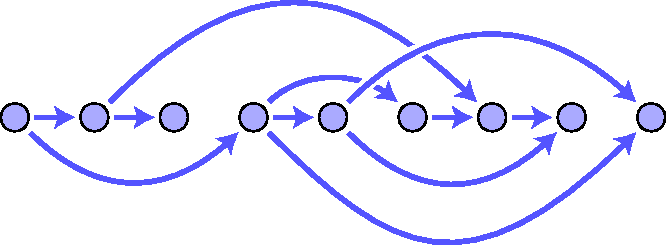
\includegraphics[width = 0.45\textwidth]{img/topo-sort}}
	{\caption{复杂依赖关系示例}\label{fig:topo-sort}}
\ffigbox[\FBwidth]%
	{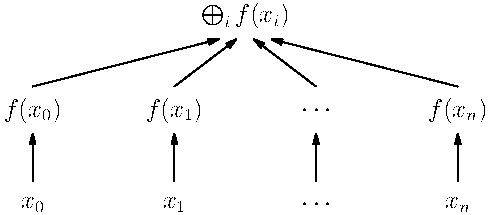
\includegraphics[width = 0.45\textwidth]{img/map-reduce}}
	{\caption{MapReduce 式依赖关系}\label{fig:map-reduce}}
\end{floatrow}
\end{figure}

类似于 \emph{EPCryst}\parencite{deng2011},\emph{decryst} 也使用等效点系组合
(EPC)法处理已指标化的数据,并把求解流程分为生成 EPC 列表、对各 EPC 进行统计
分析、对每个 EPC 进行全局最优化和导出解模型等 4 个主要步骤。因为各 EPC 上的任务
互相独立,所以 \emph{decryst} 可以并行地处理这些任务(图 \ref{fig:epc-para})。%
\textcite{deng2011}提到,\emph{EPCryst} 在 EPC 数较小(例如少于 100 个)且每个
EPC 的维数不超过 10 时特别适用;相比之下,因为 \emph{decryst} 中增量计算的应用
(参考第 \ref{sec:decr-incr} 节)以及 EPC 任务的并行化,其可以处理上千个 EPC,
每个 EPC 的维数可高达 20 以上。考虑到 EPC 法可以极大缩减搜索空间,
以及成键关系大体未知的结构 EPC 数往往很大,可以认为 EPC
任务的大规模并行化将为这类结构的求解带来前所未有的机遇。

\begin{figure}[htbp!]\bfcmd
\ffigbox%
	{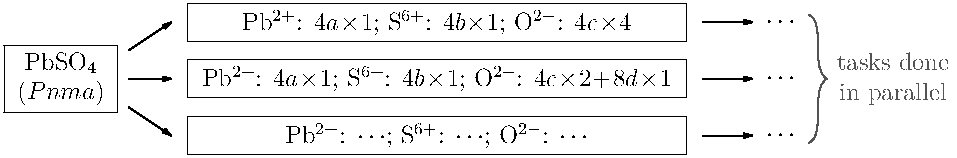
\includegraphics[width = 0.78\textwidth]{img/epc-para}}
	{\caption{EPC 的并行处理}\label{fig:epc-para}}
\end{figure}

对于维数很高的 EPC,\emph{decryst} 也可以使用并行的全局最优化,其中应用的是
\textcite{chu1999}的并行模拟退火算法,而后者又是基于 \textcite{lam1988}的
自适应模拟退火算法。Lam 算法使用连续降温,其中降温速率由若干统计参数动态控制,
而这些参数是根据相应的一套统计估计函数(statistical estimators)周期性地(每
$\tau$ 个最优化循环)计算得到的;此外为了尽量发挥最佳性能,最优化中的扰动规模
也是动态控制的,以使随机晶体模型的接受率保持在 0.44 左右。\textcite{chu1999}%
注意到模拟退火的一种物理图像是对 Boltzmann 分布的抽样,而多个抽样进程之间
可以通过周期性的状态混合来实现关联(图 \ref{fig:sa-para});
具体而言,在温度 $T$ 下选取某一进程中最近状态的概率为
\begin{equation}
	p_j = \iee ^ {-E_j / T} \Big/ \sum_j \iee ^ {-E_j / T}\mccomma
\end{equation}
其中 $E_j$ 为进程 $j$ 中最近的目标函数值。利用对各进程最近状态的周期性混合,
Boltzmann 抽样的操作可以被分配到多个进程上进行,由此便可实现对模拟退火的并行化。

\begin{figure}[htbp!]\bfcmd
\ffigbox%
	{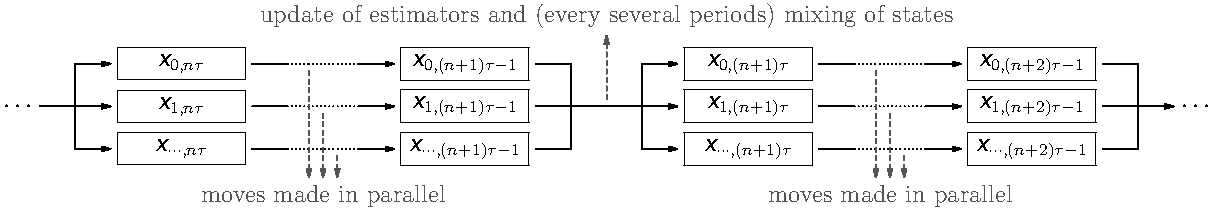
\includegraphics[width = 0.99\textwidth]{img/sa-para}}
	{\caption{模拟退火的并行化}\label{fig:sa-para}}
\vspace{\slop{-0.2em}}
\end{figure}

考虑到 \emph{decryst} 须要处理的实际需求,本人对原先并行模拟退火算法中的
一些技术细节进行了细微的改动。首先,因为晶胞具有周期边界,\emph{decryst}
中使用的搜索空间不是无限的空间,而是具有周期边界的超立方体,即多维环面(参考
第 \ref{ssec:cryst-geom} 小节);相应地,最优化中的移动步长不是从带有随机
符号的指数分布生成,而是从带有随机符号的周期指数分布(wrapped exponential
distribution)生成。其次,因为 \emph{decryst} 会随机地初始化独立原子的坐标,
所以原先算法中用于消除初态痕迹的在无限温度下进行的多次初始循环不再需要;
此外因为 \emph{decryst} 中有专门的统计分析步骤,所以用于计算统计估计函数值的
多次初始循环也不再需要。最后,为了修复或改善 \emph{decryst} 在实际测试中的
一些问题,本人还对原先算法本身进行了几项调整:

\begin{itemize}
\item 本人发现在最优化的初期,原先的算法有一定概率遇到降温过快的问题;为了解决
	这一问题,\emph{decryst} 硬性设定了模拟退火时两个相邻最优化循环中温度之比的
	上限,从而避免降温过快。本人也注意到,在最优化问题的维数很大时,特定统计参数
	的估计函数值可能被计算为浮点数中的 Inf(infinity)或 NaN(not a number),
	导致算法异常终止;为了解决这一问题,相应估计函数被适当修改\footnote{%
		具体而言,是文献\parencite[10]{lam1988}中的 $A$、$D$;同一页中的
		$\hat\mu$ 从代数上看也可能出现类似问题,因此也有类似的修改。%
	},以尽量消除计算得到的 Inf 和 NaN。此外有必要指出,上述避免降温过快的
	机制在其中也有所帮助,因为降温过快是出现 Inf 和 NaN 的一种触发条件。
\item 为了避免扰动规模 $\theta$ 在接近零时变化过于剧烈,\emph{decryst}
	中使用了基于倍数的动态控制(其中 $\rho_0$ 为最近 $\tau$
	个最优化循环所产生随机晶体模型的接受率)
	\begin{equation}
		\theta_i = \theta_{i-\tau} (\rho_0 - 0.44 + 1)\mccomma
	\end{equation}
	而不是原先基于加和的动态控制
	\begin{equation}
		\theta_i = \theta_{i-\tau} + (\rho_0 - 0.44)\mcstop
	\end{equation}
\item 在并行化中,每个进程的降温速率须为串行降温速率乘以并行进程数:例如假设串行
	温度序列为 $T_0$、$T_1$、$T_2$、$\cdots$,则原算法中双进程时每个进程的温度
	序列将为 $T_0$、$T_2$、$T_4$、$\cdots$。然而注意到一些温度值会在降温中被
	跳过,例如上述例子中的 $T_1$、$T_3$、$T_5$、$\cdots$,而这样可能造成统计估计
	函数值和实际值偏差过大,本人因此改为将串行温度序列分配到各进程,例如双进程时
	两个进程的温度序列将分别为 $T_0$、$T_2$、$T_4$、$\cdots$ 和
	$T_1$、$T_3$、$T_5$、$\cdots$。
\item 假设最优化问题的维数为 $n$,则每个最优化进程在进行 $n$ 个最优化循环之后
	会将 $n$ 个自变量的更新顺序打乱,从而消除各自变量上扰动之间的关联。这样的
	顺便带来的一个效果是每个进程中更新统计估计函数值的周期
	(即 $\tau$ 除以进程数得到的值)不再必须是 $n$ 的倍数。
\item 原先的并行化实现混合地使用了服务器{--}客户端模式和点对点模式来实现
	计算节点之间的通信。考虑到点对点模式在这一算法中对性能影响并不大,
	本人在 \emph{decryst} 的全局最优化步骤中统一采用了服务器{--}客户端模式,
	以本机为进行汇总操作的客户端、计算节点为进行独立计算的服务器端,
	利用 ZeroMQ 库进行通信(参考第 \ref{ssec:decr-arch} 小节)。
	事实上,这样也更接近于 MapReduce 的做法。
\end{itemize}

\subsection{\emph{decryst} 的软件架构}\label{ssec:decr-arch}

\emph{decryst} 是自由、开源的软件,可以从
\url{https://gitea.com/CasperVector/decryst} 获得。考虑到本人能力和精力有限,
难以承担“重复发明轮子”的成本,本人在开发 \emph{decryst} 时尽量将其设计得简洁、
灵活,从而可以关注其核心功能的开发。本人衷心希望其中应用的各种技术能够被晶体学
同行研究学习,并最终在更多的晶体学软件中得到实际的应用,由此促进晶体学软件
在自动化水平和性能上的整体进步。\emph{decryst} 由若干个部分组成(图
\ref{fig:decr-arch}),各部分的基本分工和代码组织将在本节中进行简单的介绍,
而 \emph{decryst} 的具体使用方法将在第 \ref{chap:decr-usage} 章中进行展示。

\begin{figure}[htbp!]\bfcmd
\ffigbox%
	{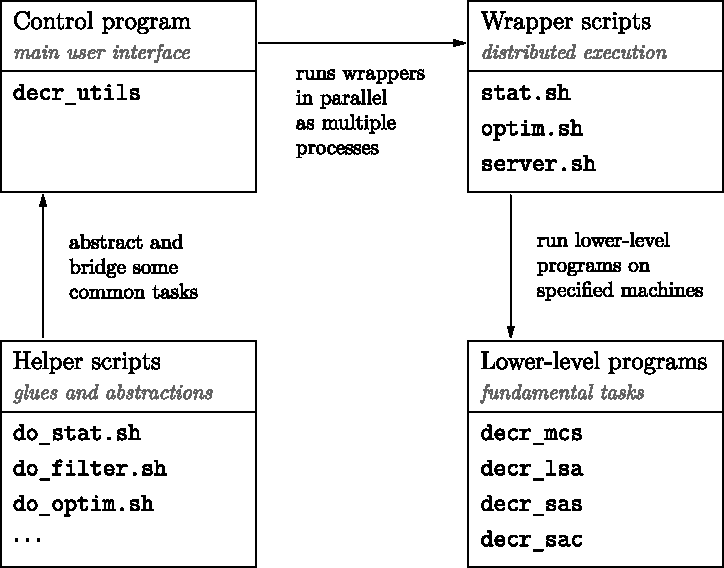
\includegraphics[width = 0.64\textwidth]{img/decr-arch}}
	{\caption{\emph{decryst} 的软件架构}\label{fig:decr-arch}}
\end{figure}

\emph{decryst} 中最基础的是一套\myterm{底层程序}(lower-level programs),其中
每一个程序实现一项底层功能:统计分析,全局最优化,等等。为了尽量发挥最佳性能,
底层程序以 C 语言写成,其代码位于 \emph{decryst} 目录树中的 \verb|src| 目录:
\begin{itemize}
\item \verb|decr_mcs|(\textbf{M}onte \textbf{C}arlo \textbf{s}tatistical
	analysis):\\实现了对单个等效点系组合(EPC)的统计分析。
\item \verb|decr_lsa|(\textbf{l}ocal \textbf{s}imulated
	\textbf{a}nnealing):\\实现了对单个 EPC 的串行模拟退火。
\item \verb|decr_sas|(\textbf{s}imulated \textbf{a}nnealing
	\textbf{s}erver):\\实现了单 EPC 并行模拟退火的服务器端。
\item \verb|decr_sac|(\textbf{s}imulated \textbf{a}nnealing
	\textbf{c}lient):\\实现了单 EPC 并行模拟退火的客户端。
\end{itemize}

建立在底层程序之上的是一个上层的\myterm{主控程序}(control program),其和
底层程序一起构成了 \emph{decryst} 的核心。主控程序调用各底层程序并和它们协作,
此外一些较为复杂但对软件总体性能影响不大的功能(特别是 EPC 的生成)
也是在主控程序中实现的。为了最大化其灵活性,主控程序以 Python 语言
写成,其代码位于 \emph{decryst} 目录树中的 \verb|python| 目录:
\begin{itemize}
\item \verb|decr_utils|:即主控程序本身;为了方便安装,本人有意将
	程序代码集中在同一文件里,但对其各部分代码进行了较为清晰的组织。
\item \verb|wyck.json|:各空间群及其中各 Wyckoff 位置的相关数据。
\item \verb|asf.json|:各元素的原子散射因子数据
	(参考第 \ref{ssec:incr-intro} 小节)。
\item \verb|rad.json|:各元素的“原子”半径(含离子半径)数据。
\end{itemize}

\myterm{包装脚本}(wrapper scripts)%
根据给定的控制参数在指定的计算节点\footnote{%
	因为 \emph{decryst} 中客户端在统计分析和全局最优化时的计算负担
	一般并不太大,所以一台机器可以同时充当客户机和计算节点。%
}上执行相应的底层程序。主控程序在调用底层程序时,事实上是通过并行地调用包装
脚本,从而使得相应的底层程序在指定的节点上执行,由此实现并行和分布式计算。
包装脚本是普通的 Unix shell 脚本,其代码位于 \emph{decryst}
目录树中的 \verb|doc/scripts| 目录:
\begin{itemize}
\item \verb|stat.sh|:用于在节点上执行 \verb|decr_mcs|。
\item \verb|optim.sh|:用于在节点上执行 \verb|decr_lsa|。
\item \verb|server.sh|:用于在节点上执行 \verb|decr_sas|。
\item \verb|ssh.sh|:以上脚本均调用该脚本以实现对远程机器的访问,
	其具体实现会调用 Unix 中的 \verb|ssh|(secure shell)程序。
\end{itemize}

\myterm{助手脚本}(helper scripts)连接不同的计算步骤,并提供上层的抽象:例如
\verb|do_rank.sh| 会根据统计分析或全局最优化的结果,利用 \textcite{deng2011}提
出的\myterm{品质因数}(figure of merit,简称 FOM)对 EPC 进行排序,从而为各 EPC
的筛选以及在后续处理中排名的确定提供依据。和包装脚本类似,助手脚本也是 shell
脚本,而其代码也位于 \emph{decryst} 目录树中的 \verb|doc/scripts| 目录;因为
助手脚本的功能较为多样,且部分脚本之间还有互相调用的关系,所以此处不再列出其
完整列表。本人有意将包装脚本和助手脚本放在 \verb|doc| 目录下,原因是它们是
\emph{decryst}灵活性的一个主要来源:在 \emph{decryst} 目前总共约 5000 行
(不计数据文件)的代码中,包装脚本和助手脚本只用了约 100 行来实现,
但在求解实际结构时用户直接调用的主要是助手脚本,而包装脚本又是
\emph{decryst} 实现分布式计算的真正基础\footnote{%
	如下文所述,ZeroMQ 只在并行模拟退火中使用,而且事实上并行模拟退火中
	也使用了 \texttt{server.sh} 来实现对服务器端的远程控制。%
}。虽然这两类脚本已经可以直接应用于实际的结构求解,但是本人希望用户能自己
读懂其中的代码,从而可以在现有脚本的基础之上进一步定制 \emph{decryst},
使之在结构测定的自动化中最大限度地发挥作用。

\emph{decryst} 的软件文档位于其目录树中的 \verb|doc| 目录:
\begin{itemize}
\item \verb|scripts| 子目录下是示例脚本,即上述的包装脚本和助手脚本。
\item \verb|usage| 子目录下是软件的用法说明,
	用户应首先阅读其中的 \verb|guide.txt|。
\item \verb|examples| 子目录下是软件用法说明中涉及的示例数据。
\end{itemize}

\emph{decryst} 还包含了几个\myterm{测评程序}(benchmark programs),包括第
\ref{ssec:cd-eval} 和 \ref{ssec:incr-obj} 小节中测评部分所涉及的一些程序,
以及一些对软件正确性的内部测试。因为须要对代码的内部结构和微观性能
进行较为准确的测试,测评程序以 C 语言写成,其代码位于
\emph{decryst} 目录树中的 \verb|bench| 目录:
\begin{itemize}
\item \verb|bench_bump| 实现了第 \ref{ssec:cd-eval} 小节中的性能测试。
\item \verb|bench_cryst| 实现了第 \ref{ssec:incr-obj} 小节中的性能测试。
\item \verb|bench_metric| 主要是对第 \ref{ssec:narrow-discus}
	小节中若干猜想的尝试性验证。
\item \verb|bench_rbtree| 是对 \emph{decryst} 在碰撞检测中所用红黑树
	(red-black tree;参考 \cite[308-338]{cormen2009})实现正确性的测试,
	因为红黑树是一个在实现时容易出细节错误的数据结构。
\end{itemize}

\emph{decryst} 为类 Unix 系统设计,而且一般不需要太多改动
就能在类似于 Cygwin 的模拟环境中运行\footnote{%
	如上文所述,虽然 \emph{decryst} 的核心部分应该不难移植到 Windows 平台,
	但是其中的包装脚本和助手脚本是普通的 Unix shell 脚本,因此也须要调用
	传统的 Unix 工具;这些工具在 Windows 下通常是由 Cygwin 等模拟环境提供,
	因此 \emph{decryst} 在 Windows 下一般需要这些模拟环境。%
};除此之外,其正确编译和安装还需要一个满足 POSIX 标准的开发环境,而
\verb|decr_sas|、\verb|decr_sac| 两个底层程序还需要 ZeroMQ 库。为了能运行
本文中的示例,用户还需要 Python、\verb|ssh| 和满足 POSIX 标准的 Unix 工具;
更加详细的安装说明可以参考 \emph{decryst} 根目录下的 \verb|README| 文件。

\section{讨论和小结}
\subsection{关于 \emph{decryst} 性能的讨论}

对于具有反演对称性的晶胞,\emph{decryst} 可以利用 (\ref{eq:cent-sym}) 式加速
结构因子的计算,从而提升最优化的性能:注意到此时只须计算半数原子所对应结构
因子的实部,计算结构因子时的性能显然是不用此公式时性能的 4 倍;因此在使用
\emph{decryst} 求解结构时,如果晶胞原点可选,应尽量使原点位于一个反演中心上。
除此之外,对于菱方晶系的结构,因为使用六方坐标系时晶胞内总原子数是使用
菱方坐标系时的 3 倍,所以为了尽量减少 \emph{decryst} 在计算原子重叠
评估函数时须要进行碰撞检测的原子对数,我们应当尽量采用菱方坐标系。

在对测量得到的衍射数据进行指标化以及确定空间群时\parencite{altomare2008a},
根据系统消光的规律对不符合实际结果的空间群进行筛除是必不可少的步骤;相应地,
在此步骤之后得到的指标化数据,例如 FullProf\parencite{rodriguez2001}产生的
\verb|.hkl| 文件中,往往包含了零强度 $hkl$ 的数据。由 (\ref{eq:total-var}) 式
可知在计算 Bragg $R$ 因子时,如果应发生系统消光的一些 $hkl$ 实际测得的强度
确实为零,那么在计算中忽略这些 $hkl$ 不会对得到的 $R$ 值产生影响。因此,
在将指标化数据转换到方便 \emph{decryst} 读取的格式时,我们可以利用一些
自动化工具删除数据中符合消光规律的零强度 $hkl$,从而一定程度地提升最优化
的性能;类似地,在适当的条件下,可以酌情忽略高角度的 $hkl$。

考虑 $R\bar3c$ 空间群(菱方坐标系,忽略反演对称)的对称操作:
\begin{gather}
	(x,y,z)\mccomma (z,x,y)\mccomma (y,z,x)\mccomma\nonumber\\
	(\bar{z}+\frac12,\bar{y}+\frac12,\bar{x}+\frac12)\mccomma
	(\bar{y}+\frac12,\bar{x}+\frac12,\bar{z}+\frac12)\mccomma
	(\bar{x}+\frac12,\bar{z}+\frac12,\bar{y}+\frac12)\mcstop
\end{gather}
注意到上述坐标中有大量重复的表达式,例如 $x$、$y$、$z$、$\bar{x}+\frac12$、%
$\bar{y}+\frac12$、$\bar{z}+\frac12$ 分别出现了 3 次,我们似乎可以通过将
表达式分组,然后在其自变量发生改变时只求值一次,后续用到时直接使用求出的值。在
\emph{decryst} 的全局最优化步骤中,考虑到两个相邻的最优化循环里晶体模型之间的差
别一般只在于单个独立原子中一个坐标的改变,这样似乎会比较有利:除了在计算结构因子
时的便利之外,在使用 sweep and prune(SAP,参考第 \ref{ssec:cryst-sap} 小节)
时,利用上述分组,我们可以只对受坐标变动影响的那些投影区间重新进行碰撞检测。
然而,在每次计算目标函数时,原子坐标事实上是在被计算一次之后便用于计算许多
$hkl$ 的结构因子,因此原子坐标的计算开销在目标函数的计算开销中所占比例不大;
此外如 \ref{ssec:incr-obj} 小节所述,\emph{decryst} 事实上并未使用 SAP,
因此以上性能调优技术带来的性能提升非常有限,所以最终未被采用。

\subsection{关于浮点数求和的讨论}

如第 \ref{ssec:incr-obj} 小节所述,\emph{decryst} 目前在增量求和时通过在内部
使用定点数的方式来绕过浮点数求和的误差积累问题;这样做并不完美,因为定点数精度
也有限,在加法超过其上界时会溢出到下界(相应地,减法可能会溢出到上界)。为了
防止溢出,\emph{decryst} 对浮点数 $x_\text{float}$ 到定点数 $x_\text{fix}$
之间的换算常数 $c \approx x_\text{fix} / x_\text{float}$ 进行了限制,以保证
求和结果的定点数表示即使在最坏情形下也不会发生溢出。然而,因为
\begin{equation}
	c \approx M_\text{fix} \Big/ \sum_i |x_{\text{float},i}|_\text{max}
\end{equation}
(其中 $M_\text{fix}$ 为定点数所用整数类型绝对值的上界),所以 $c$ 的值在
被求和数的个数很大时会很小,从而增大换算时的截断误差;这在晶胞内总原子数
$n$ 很大时尤其值得注意,因为此时被求和数的个数是 $n (n - 1) / 2$。

另外一种可能可行的思路是直接使用增量的浮点求和,但周期性地从头求和,从而
避免求和误差的无界积累;事实上,\emph{decryst} 在并行模拟退火(参考第
\ref{ssec:decr-para} 小节)中进行状态混合时,在很大程度上已经是从头计算晶体
模型的目标函数了。然而,在各种条件下如何妥善确定从头求和的周期,
还有这一周期和 \textcite{lam1988}的算法中统计估计函数的更新周期以及
\textcite{chu1999}的算法中进行状态混合的周期之间的关系应当如何把握,
这些问题在应用上述思路之前都需要仔细考虑。

使用高精度的浮点数可以大大减轻浮点数求和中的误差积累问题,但在 \emph{decryst}
中仍无法完全根治这一问题,因为其中浮点数增量求和的误差积累是无上界的,只是在用
高精度浮点数时每次求和的相对误差被很大程度地缩小了。当然,如果将高精度浮点数和
以上周期性从头求和的思路同时使用,对误差积累进行有效控制仍是很有希望做到的;
类似地,对于上文所述晶胞内总原子数 $n$ 很大的情形,如果以高精度的整数为定点数
的基础,截断误差对最终计算结果的影响应该也是可以控制在一个满意的范围之内的。

\subsection{关于等效点系组合生成算法的讨论}\label{ssec:epc-discus}

如第 \ref{sec:dspace-epc} 节所述,在早期的正空间法工作中,晶体学家以极其
具有技巧性的方式对等效点系组合(EPC)进行筛选。例如在\textcite{lu1965}关于
\ce{V2Ga5}($P4/mbm$,$Z = 2$)的工作中,作者首先根据晶胞化学式和各 Wyckoff
位置的多重度列出了可能的多重度组合:
\begin{multicols}{2}
\begin{enumerate}[label = {\Alph*.}, leftmargin = 2\parindent]
	\item $8 + 4 + 2$;
	\item $8 + 2 + 2 + 2$;
	\item $4 + 4 + 4 + 2$;
	\item $4 + 4 + 2 + 2 + 2$;
	\item $4 + 2 + 2 + 2 + 2 + 2$;
	\item $2 + 2 + 2 + 2 + 2 + 2 + 2$。
\end{enumerate}
\end{multicols}
{\noindent}因为固定 Wyckoff 位置只有 4 个,所以组合 E、F 首先被排除;接下来,因
为 $c$ 方向空间有限,$2a$、$2b$ 互斥且 $2c$、$2d$ 互斥,所以组合 B、D 也被排除。
考虑到 $c$ 方向只能容纳一个原子,$4e$、$4f$ 不可用,在多重度为 4 的 Wyckoff 位置
中只能选择 $4g$ 或 $4h$,而这导致组合 C 在 $\{220\}$ 平面一定会发生原子重叠,
所以组合 C 也被排除。对于组合 A,在排除等价 EPC 之后,作者根据特定衍射峰的强度
对剩余的可行 EPC 进行了最终的筛选。有必要指出,在不考虑除固定位置约束之外的原子
重叠因素时,\ce{V2Ga5} 总共有 428 个可选 EPC,因此仅通过人工计算将其
EPC 筛选至只剩一个已经可谓是惊人的工作。

以上的技巧并未完全在 \emph{decryst} 中得到应用。首先,以上先生成多重度组合再
生成 EPC 的思路并未在 \emph{EPCryst}\parencite{deng2011}或 \emph{decryst}%
(参考第 \ref{ssec:incr-epc} 小节)中采用,这是因为以上思路实现起来明显更加
复杂,但在算法的时间和空间复杂度上似乎并没有很大的改善。本人认为这并不说明以上
思路已经过时,而是说明其在当前的应用场景下没有充分发挥优势;在其它一些应用
场景下,这一思路仍有可能体现其独特的价值。此外,以上筛选中用到了涉及多于一个
Wyckoff 位置的占据数约束,例如“$2a$、$2b$ 位置总共最多占据一次”,
而 \emph{decryst} 目前尚不支持这样的约束。

此外有必要指出,利用第 \ref{ssec:incr-epc} 小节中剪枝的思路,从原则上看应该是
可以在生成 EPC 时根据原子重叠等因素对其进行实时筛选的,关于这一点的详细讨论
可以参考第 \ref{ssec:prune-discus} 小节。

\subsection{其它讨论}

对于在正空间法中主要以原子坐标作为全局最优化中自变量的结构测定软件,例如
\emph{FOX}\parencite{favre2002}、\emph{FraGen}\parencite{li2012}等,利用
类似于第 \ref{ssec:incr-obj} 小节所述的方法应该不难实现目标函数的增量计算,
其中也包括比 (\ref{eq:obj-func}) 式更为复杂的一些目标函数(例如考虑了配位数、
键价、配位多面体形状等等因素的那些)。然而,增量计算对于主要面向分子晶体的
正空间法软件可能并不太适用,因为这一类软件中大量使用键长、键角等等作为
最优化的自变量,而这常常会导致单个自变量的变化影响到所有原子的坐标。

尽管多数晶体学软件并不采用等效点系组合法,可完美并行的任务仍是广泛存在的:
例如第 \ref{chap:decr-usage} 章中将介绍须要多次执行全局最优化步骤,并在其
所得解中挑选最优解的复杂结构;显然,各次最优化之间是完全独立的,因此类似于第
\ref{ssec:decr-para} 小节中那样可以完美并行。最优化算法的并行化也具有重要意义:
例如结构精修中最优化算法的并行化将可以明显缩短用户等待精修结果的时间,
而本人注意到 \textcite{eremenko2017}近期的工作已经在往这一方向努力;此外,
一些最优化算法本身就比较容易并行化,例如 \emph{FOX} 中采用的并行回火算法。

本人最近也注意到,基于 \textcite{chu1999}算法中 Boltzmann 状态混合的思路,
\textcite{lou2016}近期提出了一种新的并行模拟退火算法。新算法在实现上明显比
原算法要简单,但却有更高的并行效率;但为了提升并行效率,其不再使用自适应的
模拟退火,这使其串行性能并不优于原算法。在未来版本的 \emph{decryst} 中,
本人有可能采用上述新算法来实现并行的全局最优化;
当然,并行回火等算法也将在考虑之列。

\subsection{本章小结}

基于第 \ref{chap:cryst-cd} 章中的原子重叠排除机制,本人开发了 \emph{decryst}
这一套利用正空间法和等效点系组合(EPC)法从指标化的粉末衍射数据求解晶体结构的
软件。受 Unix 中 \verb|make| 程序的启发,本人在 \emph{decryst} 中首次将增量计算
的思想以一种具有通用性的方式应用于全局最优化步骤中,使其性能得到了明显的提升;
\emph{decryst} 也使用一种增量算法生成 EPC,这不仅极大降低了其内存需求,而且
为在生成 EPC 时对其进行实时筛选做了准备。根据 \emph{decryst} 中计算步骤的相关
属性,本人在其中加入了对并行和分布式计算的支持,使之可以通过同时利用多个处理器
实现对晶体结构测定的进一步加速;考虑到同一结构的各 EPC 互相独立,而且 EPC 数在
多数有意义的情形下都相当大,\emph{decryst} 中统计分析和全局最优化任务的并行化
将为求解成键关系总体未知的结构带来前所未有的机遇。

\begin{rquote}{0.5\textwidth}
	\begingroup\setmainfont{GFS Didot}\itshape
	Ὁ βίος βραχύς, ἡ δὲ τέχνη μακρή.\endgroup\\
	(Vita brevis, ars longa.)
\end{rquote}
\rightline{--- Greek aphorism}

% vim:ts=4:sw=4

	% Copyright (c) 2014,2016,2018 Casper Ti. Vector
% Public domain.

\chapter{\emph{decryst} 的使用方法和常用技巧}\label{chap:decr-usage}

本章将以 AMCSD 数据库\parencite{downs2003}中若干个不同晶系和复杂度的结构为例,
循序渐进地演示 \emph{decryst} 的基本用法和常用技巧;目前 \emph{decryst} 中自带了
\ce{Al2O3}(AMCSD 代号:0009325)、\ce{As2S3}(0010733)、\ce{PbSO4}(0005558)
和“0009563”等 4 个结构作为示例。此外,因为有一位用户在 \emph{decryst} 的试用阶段
建议再增加几个不同晶系和复杂度的示例,本人在 AMCSD 中搜索 $a$、$b$、$c$ 均介于
\SIrange{8}{16}{\angstrom} 的结构,在第一页结果中去除过于简单或过于复杂的
结构后选取了 “0000158”“0000219”“0000220”“0000428”“0000589” 等 5 个结构。
各代号所对应的化学式见相应小节;在本章的演示中,以上所有
结构在求解时均忽略 H 原子\footnote{%
	有必要指出,在结构精修中利用 X 射线衍射数据处理 H 原子是可行且
	有很强实际意义的,相关研究可参考文献\parencite{cooper2010}。%
},所有时间测量均在 Intel i7-3720QM CPU 上进行。

\section{\emph{decryst} 的基本用法}

在本节中,第 \ref{ssec:decr-fmt} 小节将介绍 \emph{decryst} 中主控程序(参考第
\ref{ssec:decr-arch} 小节)的输入格式,第 \ref{ssec:decr-base} 小节将演示
主控程序的用法,以及用 \emph{decryst} 进行结构测定的基本流程。在此基础之上,
第 \ref{ssec:decr-auto} 小节将讨论对全局最优化步骤中得到的评价指标相近的解进行
手工(目视)筛选的技术,并演示结合自动化工具使用 \emph{decryst} 的基本方法。第
\ref{ssec:epc-rank} 小节将初步演示和讨论对等效点系组合(EPC)进行筛选的方法。

\subsection{\emph{decryst} 中主控程序的输入格式}\label{ssec:decr-fmt}

如第 \ref{ssec:decr-arch} 小节所述,\emph{decryst} 中面向用户的核心接口由
主控程序 \verb|decr_utils| 提供。因此为了使用 \emph{decryst} 进行结构测定,
我们最先须要编写的是 \verb|decr_utils| 的输入文件(称为 \myterm{decr 文件},
详细格式参考 \verb|doc/usage/format.txt|)。首先以
\ce{Al2O3} 结构为例,其 decr 文件如下所示\footnote{%
	AMCSD 中的衍射数据不含半高宽(FWHM)字段,
	因此本章所有 decr 文件中 FWHM 值均为粗略的估计值。%
}:
\begin{Verbatim}
\cm{# (Lines beginning with `#' are comments and are ignored.)}
\cm{# ID of space group, (a, b, c), (alpha, beta, gamma).}
167a	4.7602 4.7602 12.9933	90 90 120
\cm{# Combination factor `mu', and some other control parameters.}
0.25 0.75 0.875	0.5 1.0
\cm{# Global EPC constraints (`--' for the defaults).}
--

\cm{# Atom species, number of atoms, EPC constraints, already}
\cm{# guessed EPCs with unknown coordinates (`--' for none).}
Al3+	12	--	--
O2-	18	--	--
\cm{# Pairwise zoom factors.}
1.6:0-0
\cm{# Wyckoff positions and coordinates for already solved atoms.}
\cm{#0@c1}	\cm{0}	\cm{0}	\cm{0.14784}

\cm{# Data for individual reflections:}
\cm{# 2-theta, FWHM, hkl, multiplicity, intensity.}
25.59	0.2	0 1 2	6	61.91
35.17	0.2	1 0 4	6	96.62
\cm{# (... further data lines left out for brevity ...)}

\end{Verbatim}

其中指定各 $hkl$ 所对应衍射数据的那些行以及指定空间群和晶胞参数的一行意义应该
很明显,唯一需要注意的是空间群的代号须要根据 \verb|wyck.json| 进行设定,例如
上述示例中 \verb|167a| 表示采用 $R\bar3c$ 空间群的六方表示。晶胞参数之后的一行
数据指定结构测定中使用的一些参数(详见 \verb|format.txt|),
其中最重要的是第 1 个和第 4 个:前者是组合因子 $\mu$(参考第
\ref{ssec:eval-func} 小节),而后者是 Lorentz{--}极化因子公式\footnote{%
	这一公式和国际晶体学表\parencite[620]{prince2004}中的公式是兼容的:
	事实上,对前者而言的 $p$ 正是对后者而言的 $A / (1 + A)$。%
}中的参数 $p$:
\begin{equation}
	LP = \frac{(1 - p) + p\cos^2 2\theta}{\sin2\theta \sin\theta}\mcstop
\end{equation}
$\mu$ 等参数之后的一行数据指定对晶胞中总 EPC 的额外约束(参考第
\ref{ssec:incr-epc} 小节),其写法形如 \verb|0-3 1-2|,其中每个字段对应于一个
Wyckoff 位置($a$、$b$、$\cdots$,其顺序根据 \verb|wyck.json| 中指定空间群
Wyckoff 位置的列表确定)总占据数的下限和上限。下限和上限都可省略,表示不对相应值
设定额外约束;此外,\verb|decr_utils| 会自动设定所有固定 Wyckoff 位置的占据数
上限不超过 1。最后,如果所有 Wyckoff 位置的总占据数均无额外约束,那么设定这一
约束的行可以被简写为“\verb|--|”,正如上述 \ce{Al2O3} 的例子所示。

晶胞化学式和对单元素 EPC 的约束由形如
\begin{Verbatim}
Al3+	12	--	--
\end{Verbatim}
的数据行指定。其中第 1 个字段是元素的代号,其半径\footnote{%
	中性原子采用共价半径\parencite{cordero2008},
	而离子采用离子半径\parencite{shannon1976}。%
}和散射因子数据分别会从 \verb|rad.json| 和 \verb|asf.json| 中读取;两者
所需元素代号不同时可使用形如 \verb|S6+;S| 的写法,而“混合元素”可用形如
\verb|0.6Fe2+,0.3Fe3+| 的写法来指定。第 2 个字段是晶胞中相应元素的
总原子数。第 3、4 个字段分别指定相应元素占据数的下限和上限,
写法形如 \verb|a2b1|(注意这和第 \ref{ssec:incr-epc} 小节中所用
EPC 表达式的相似性);其中未写出的 Wyckoff 位置均视作未设定额外约束,
而所有 Wyckoff 位置均无额外约束时相应字段可写为“\verb|--|”。

对缩放因子(参考第 \ref{ssec:cryst-sap} 小节,默认为 1)由形如
\begin{Verbatim}
1.1:0,1-1,2	1.2:2-2
\end{Verbatim}
的数据行\footnote{%
	即输入文件中除了空行和(以“\texttt{\#}”开头的)注释行之外的那些行。%
}指定,其中每个字段中“\verb|:|”之前为缩放因子的值,之后为被赋予相应
缩放因子的原子对:\verb|0,1-0,1| 会被展开为 \verb|0-0|、\verb|0-1| 和
\verb|1-1|。这里元素的编号根据晶胞化学式部分各元素被定义的顺序而定,
从零开始计数:例如在上述的 \ce{Al2O3} 示例中,\verb|0-0| 表示的是
\ce{Al^{3+}}--\ce{Al^{3+}} 原子对。已知位置的独立原子\footnote{%
	只有部分坐标已知的独立原子也可以用这种数据行表示,
	详见 \texttt{format.txt}。%
}由形如
\begin{Verbatim}
0@c1	0	0	0.14784
\end{Verbatim}
的数据行指定。在上述的 \ce{Al2O3} 示例中,以上数据行表示第 1 种元素(编号为 0,
即 \ce{Al^{3+}})占据 1 组 $c$ 位置,其中一个原子的坐标为 $(0, 0, 0.14784)$。

关于 \emph{decryst} 所用各类输入文件的格式,最后须要指出一些小但值得注意的技术
细节。首先,所有输入文件都只支持 Unix 中常用的 LF(\verb|\n|)换行符,而不支持
Windows 中常用的 CRLF(\verb|\r\n|)换行符,因此用户在 Windows 上编写的输入文件
一般须要经过 \verb|dos2unix| 等工具的转换。其次,输入文件中的空行(包括文件
末尾的空行,例如上述 \ce{Al2O3} 示例中的最后一行)具有特殊作用,不可随意添加或
删除。最后,数据行中空白字符(空格和制表符 \verb|\t|)可以混合使用,但建议
在不同类型的行中有规律地使用空白字符,从而方便利用文本处理工具进行自动化的
修改(参考第 \ref{ssec:heavy-atom} 和 \ref{ssec:epc-filter} 小节)。

\subsection{基本求解流程:以 \ce{Al2O3} 和 \ce{As2S3} 为例}\label{ssec:decr-base}

如第 \ref{ssec:decr-para} 小节所述,\emph{decryst} 将结构测定划分为生成
EPC 列表、对各 EPC 进行统计分析、对每个 EPC 进行全局最优化和导出解模型等
4 个主要步骤。这里先继续以 \ce{Al2O3} 的结构测定为例;在编写完 decr
文件之后,用以下命令即可生成 EPC 列表:
\begin{Verbatim}
\cm{$} decr_utils comb /path/to/Al2O3.txt | tee combs.list
\end{Verbatim}
其输出(称为 \myterm{combs 文件},详见 \verb|format.txt|)应如下所示:
\begin{Verbatim}
\cm{>} 0@a1b1,1@d1.cr	0@a1b1,1@d1
\cm{>} 0@a1b1,1@e1.cr	0@a1b1,1@e1
\cm{>} ...
\end{Verbatim}
其中两个字段分别为该 EPC 所对应的文件名和表达式。有必要特别提请注意的是,combs
文件中的 EPC 只考虑未分配到任何 Wyckoff 位置的原子,而且 decr 文件中已知 Wyckoff
位置的两种原子是被分开计数的:例如要是 decr 文件中指定了某元素的占据数上限
约束为 \verb|c3|、下限约束为 \verb|c1|,且该元素还有一个坐标已知的 \verb|c1|
占据,那么该元素在 combs 文件列出的 EPC 中最多会占据 1 组 $c$ 位置。此外,如果
所有原子均已在 decr 文件中分配到确定的 Wyckoff 位置,那么在此条件下只可能生成一个
“空的”EPC,而该 EPC 会被显示为 \verb|nil|。有了 combs 文件,我们就可以
实际生成各 EPC 所对应的用于 \emph{decryst} 中底层程序的输入文件\footnote{%
	这里的 EPC 文件名和下文中各 EPC 的全局最优化参数都是可以修改的;
	分两步生成 cryst 文件是为了在分步求解复杂结构时(例如在使用重原子法时,
	参考第 \ref{sec:decr-adv} 节)方便管理各步骤所需的输入文件。%
}(称为 \myterm{cryst 文件}\footnote{%
	本文中的各个示例不涉及其格式,因此本文不对其进行讨论,
	但其细节可参考 \texttt{format.txt};其余未注明
	“详见 \texttt{format.txt}”等字样的输入文件也类似。%
}):
\begin{Verbatim}
\cm{$} decr_utils dump /path/to/Al2O3.txt < combs.list | tee crysts.list
\end{Verbatim}
其输出(称为 \myterm{crysts 文件},详见 \verb|format.txt|)应如下所示:
\begin{Verbatim}
\cm{>} 0 0 - - - - -	0@a1b1,1@d1.cr
\cm{>} 1 1000 100 0.01 - - -	0@a1b1,1@e1.cr
\cm{>} ...
\end{Verbatim}
在 crysts 文件中,最后一个字段是 cryst 文件的文件名(可以注意到相应的文件已在
当前目录生成),第一个字段是相应 EPC 的维数;第 2--4 个字段分别为统计分析中的
样本数和 Lam 算法(参考第 \ref{ssec:decr-para} 小节)中的
$\tau$、$\lambda$ 参数\footnote{%
	其中零维 EPC 的样本数显示为 0(实际为 1)是出于方便自动化
	的考虑;这些 EPC 的 $\tau$ 和 $\lambda$ 显示为“\texttt{-}”,
	表示这两个参数无意义,因为这些 EPC 不需要全局最优化。%
}(后者取更小的值时,最优化会更精细但更耗时);第 5--7 个字段分别为相应
EPC 所产生晶体模型目标函数值 $E$ 的平均值、标准差和已知最佳值
(目前均显示为“\texttt{-}”,表示这些参数的值未知)。

\emph{decryst} 在对 EPC 进行统计分析和全局最优化时支持并行和分布式计算,而相应的
设定是通过 \myterm{hosts 文件}进行的,其详细格式参考 \verb|format.txt| 及其同一
目录中的 \verb|cmdline.txt|。\verb|doc/example/hosts.conf| 是 \emph{decryst}
自带的一个和 \verb|doc/scripts| 目录中脚本兼容的示例 hosts 文件,用户可根据自身
需求对其进行修改。此外,为了能正确调用包装脚本(参考第 \ref{ssec:decr-arch}
小节),\verb|scripts| 目录须要在搜索路径 \verb|$PATH| 中,而且
\verb|decr_mcs|、\verb|decr_lsa| 和 \verb|decr_sas| 须要安装到所有远程机器上。
在正确进行以上配置之后,我们便可以对上一步生成的 cryst 文件进行统计分析:
\begin{Verbatim}
\cm{$} decr_utils stat stat.sh /path/to/hosts.conf < crysts.list |
  tee crysts.stat
\end{Verbatim}
其输出应大致如下:
\begin{Verbatim}
\cm{>} 0 0 - - - - 0.385611	0@a1b1,1@d1.cr
\cm{>} 2 1000 200 0.01 0.530822 0.165276 0.045932	0@c1,1@e1.cr
\cm{>} ...
\end{Verbatim}
可见平均值、标准差、最佳值已被实际值取代;对于零维 EPC,只有最佳值有意义,
因此平均值和标准差仍显示为“\texttt{-}”。在获得统计分析的结果之后,
我们便可以进行全局最优化:
\begin{Verbatim}
\cm{$} decr_utils optim optim.sh /path/to/hosts.conf < crysts.stat |
  tee crysts.optim | sort -k7g
\end{Verbatim}
其输出应大致如下:
\begin{Verbatim}
\cm{>} 2 1000 200 0.01 0.530822 0.165276 0.0298237	0@c1,1@e1.cr
\cm{>} 1 1000 100 0.01 0.473024 0.157376 0.209828	0@a1b1,1@e1.cr
\cm{>} ...
\end{Verbatim}
注意其中最佳值已被替换为全局最优化步骤所得解模型的相应值,以及当前目录中生成了
用于记录全局最优化过程的 \verb|.log| 文件(称为 \myterm{crlog 文件}),如
\verb|0@c1,1@e1.log|。此外因为零维 EPC 不需要全局最优化,所以 crysts 文件中的
相应行会被 \verb|decr_utils| 的 \verb|optim| 子命令原样输出。

如上述输出(已用 \verb|sort| 命令排序)所示,\verb|0@c1,1@e1| 是 \ce{Al2O3}
唯一可行的 EPC。最后,我们可以将全局最优化的结果和原 decr 文件合并,
以产生各解模型所对应的 decr 文件和 CIF 文件:
\begin{Verbatim}
\cm{$} decr_utils merge /path/to/Al2O3.txt < combs.list
\end{Verbatim}
其输出应如下所示:
\begin{Verbatim}
\cm{>} 0@a1b1,1@d1.cr
\cm{>} 0@a1b1,1@e1.cr
\cm{>} ...
\end{Verbatim}
正确解所对应的 decr 文件和 CIF 文件分别是 \verb|0@c1,1@e1.txt|
和 \verb|0@c1,1@e1.cif|,后者可以直接在可视化软件中查看。
以上求解过程(除去人工步骤之后)耗时不到 \SI{1}{\second}。

\ce{As2S3}($P2_1/c$)的 decr 文件如下所示(注意其中因为缺少 \ce{As^{3+}}、%
\ce{S^{2-}} 的原子散射因子数据而采用了电中性 As、S 原子的数据,
参考第 \ref{ssec:decr-fmt} 小节):
\begin{Verbatim}
\cm{# sg, abc, angles; ctl, extra; limits.}
14a	4.256 9.577 12.191	90 109.75 90
0.25 0.75 0.875	0.5 1.0
--

\cm{# rad/asf, n, limits, comb.}
As3+;As	8	--	--
S2-;S	12	--	--

\cm{# 2theta, fwhm, hkl, mult, val.}
12.04	0.1	0 1 -1	4	12.34
18.02	0.1	0 1 -2	4	15.82
\cm{# (... further lines omitted ...)}
\end{Verbatim}
仿照以上步骤,其结构可以用完全类似的方法进行求解,除去人工步骤之后耗时约
\SI{15}{\second}。在求解的过程中,可以注意到正确 EPC \verb|0@e2,1@e3| 耗时远多于
其它所有 EPC,因为其维数(15)明显高于其它 EPC(均不超过 12);此外,\ce{As2S3}
有时一次全局最优化不能得到正确的解模型,需要多次求解。对于这类 EPC,并行的
全局最优化可以用于缩短单个 EPC 求解所需的时间,例如对 \ce{As2S3}
的 \verb|0@e2,1@e3| EPC 可以使用以下命令:
\begin{Verbatim}
\cm{$} grep 0@e2,1@e3 < crysts.list |
  decr_utils poptim server.sh hosts.conf | tee 0@e2,1@e3.log
\end{Verbatim}
需要注意的是 \verb|decr_utils| 的 \verb|poptim| 子命令只接受单行的 crysts 文件,
而且输出的是 crlog 文件而非 crysts 文件,因此用户须要自行管理其输出。

\subsection{实际求解:以“0000220”和“0000589”结构为例}\label{ssec:decr-auto}

“0000220”结构($Ia\bar3d$)的 decr 文件如下所示(注意其中一价原子被表示为
\verb|Li1+|、\verb|Na1+| 和 \verb|F1-|,这和 \verb|wyck.json| 是一致的,
参考第 \ref{ssec:decr-fmt} 小节):
\begin{Verbatim}
\cm{# sg, abc, angles; ctl, extra; limits.}
230	12.122 12.122 12.122	90 90 90
0.25 0.75 0.875	0.5 1.0
--

\cm{# rad/asf, n, limits, comb.}
Li1+	24	--	--
Na1+	24	--	--
Al3+	16	--	--
F1-	96	--	--
\cm{# zooms.}
1.4:2-2

\cm{# 2theta, fwhm, hkl, mult, val.}
17.92	0.2	2 1 1	24	11.87
20.73	0.2	2 2 0	12	100.00
\cm{# (... further lines omitted ...)}
\end{Verbatim}
该结构可以使用第 \ref{ssec:decr-base} 小节中的方式求解:其总 EPC 数为 28,单个
EPC 维数为 2--3,除去人工步骤之后求解总耗时约 \SI{5}{s},可直接得到目标函数值
$E = 0.0278$ 的正确解;正确 EPC 为 \verb|0@d1,1@c1,2@a1,3@h1|,
而其余 EPC 所得解的 $E$ 值至少为 0.11。

“0000589”结构($Pm\bar3m$)的 decr 文件如下所示:
\begin{Verbatim}
\cm{# sg, abc, angles; ctl, extra; limits.}
221	10.358 10.358 10.358	90 90 90
0.25 0.75 0.875	0.5 1.0
--

\cm{# rad/asf, n, limits, comb.}
Li1+	1	--	--
K1+	6	--	--
Fe2+	24	--	--
S2-;S	26	--	--
Cl1-	1	--	--

\cm{# 2theta, fwhm, hkl, mult, val.}
8.54	0.2	1 0 0	6	56.41
12.08	0.2	1 1 0	12	38.10
\cm{# (... further lines omitted ...)}
\end{Verbatim}
该结构的总 EPC 数为 2416,单个 EPC 维数为 5--9。其依然可以
按照上述各结构的方式求解,所得结果通常大致如下\footnote{%
	因为所使用算法中随机因素的缘故,实际结果中 $E \approx 0.075$ 的 EPC 数可能
	发生一定程度的浮动;在使用 \emph{decryst} 默认的参数时,其一般为 1--2。%
}:
\begin{Verbatim}
\cm{>} [...] 0.677702 0.0638962 0.0456528	0@b1,1@f1,2@m1,3@e1g1h1,4@a1.cr
\cm{>} [...] 0.676874 0.0680791 0.0469421	0@b1,1@e1,2@m1,3@f1g1h1,4@a1.cr
\cm{>} [...] 0.682297 0.0653026 0.0740492	0@a1,1@e1,2@m1,3@f1g1h1,4@b1.cr
\cm{>} [...] 0.686445 0.060813 0.0749921	0@a1,1@f1,2@m1,3@e1g1h1,4@b1.cr
\cm{>} [...] 0.697594 0.0678327 0.133365	0@a1,1@f1,2@m1,3@e1g1j1,4@b1.cr
\cm{>} ...
\end{Verbatim}
从 $E$ 值可见只有前 4 个 EPC 可能是合理的,又由 $(1/2, 1/2, 1/2)$ 平移使
$Pm\bar3m$ 空间群中 $a/b$、$c/d$、$e/f$、$i/j$、$k/l$ 位置互变并保持其它
Wyckoff 记号不变可知这 4 个 EPC 是两对等价 EPC。在可视化软件中查看这两对
EPC 生成的解,可见在 \verb|0@b1,1@f1,...| 和 \verb|0@a1,1@e1,...|
的解中 \ce{Cl-} 均被 \ce{S^{2-}} 配位(图 \ref{fig:589-sol}(c,d)),
这显然是错误的。在 \verb|0@b1,1@e1,...|(图 \ref{fig:589-sol}(a))和
\verb|0@a1,1@f1,...|(图 \ref{fig:589-sol}(b))的解中,即使不考虑后者
\ce{K+}--\ce{Fe^{2+}} 键长过短的问题,只根据 $E$ 值也可以知道前者是
唯一合理的解。除去人工步骤之后,“0000589”求解总耗时约 \SI{5}{\minute}。

\begin{figure}[htbp!]\bfcmd
\ffigbox{\begin{subfloatrow}
	\setlength{\columnsep}{1.5em}
	\ffigbox[0.32\textwidth]%
		{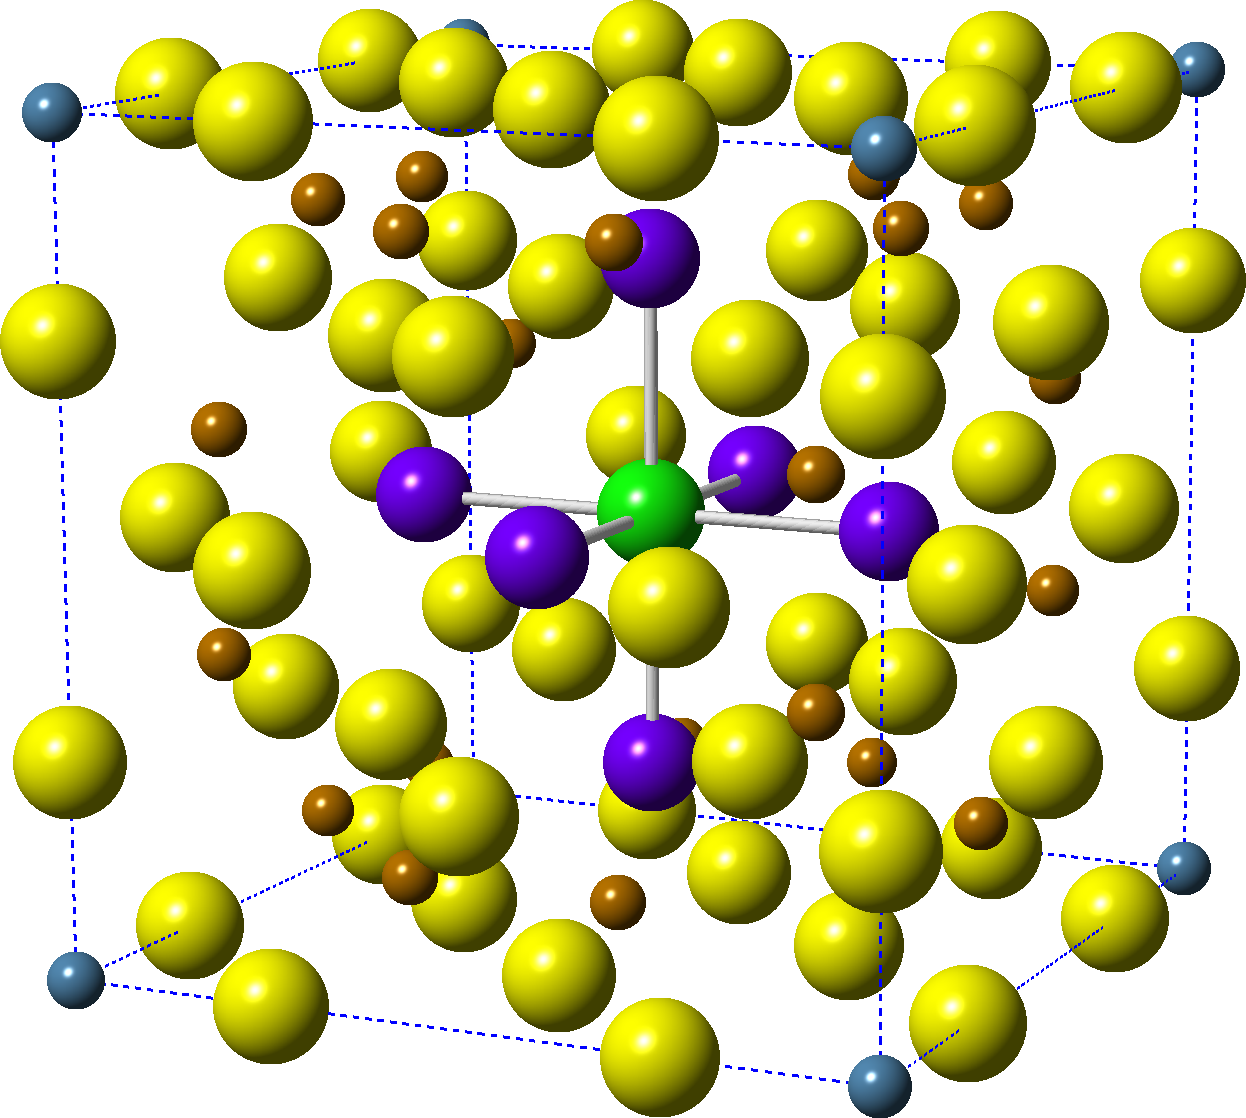
\includegraphics[height = 0.25\textwidth]{img/589-sol-1}}%
		{\caption{\texttt{0@a1,1@f1}($E = 0.0469$)}}
	\ffigbox[0.32\textwidth]%
		{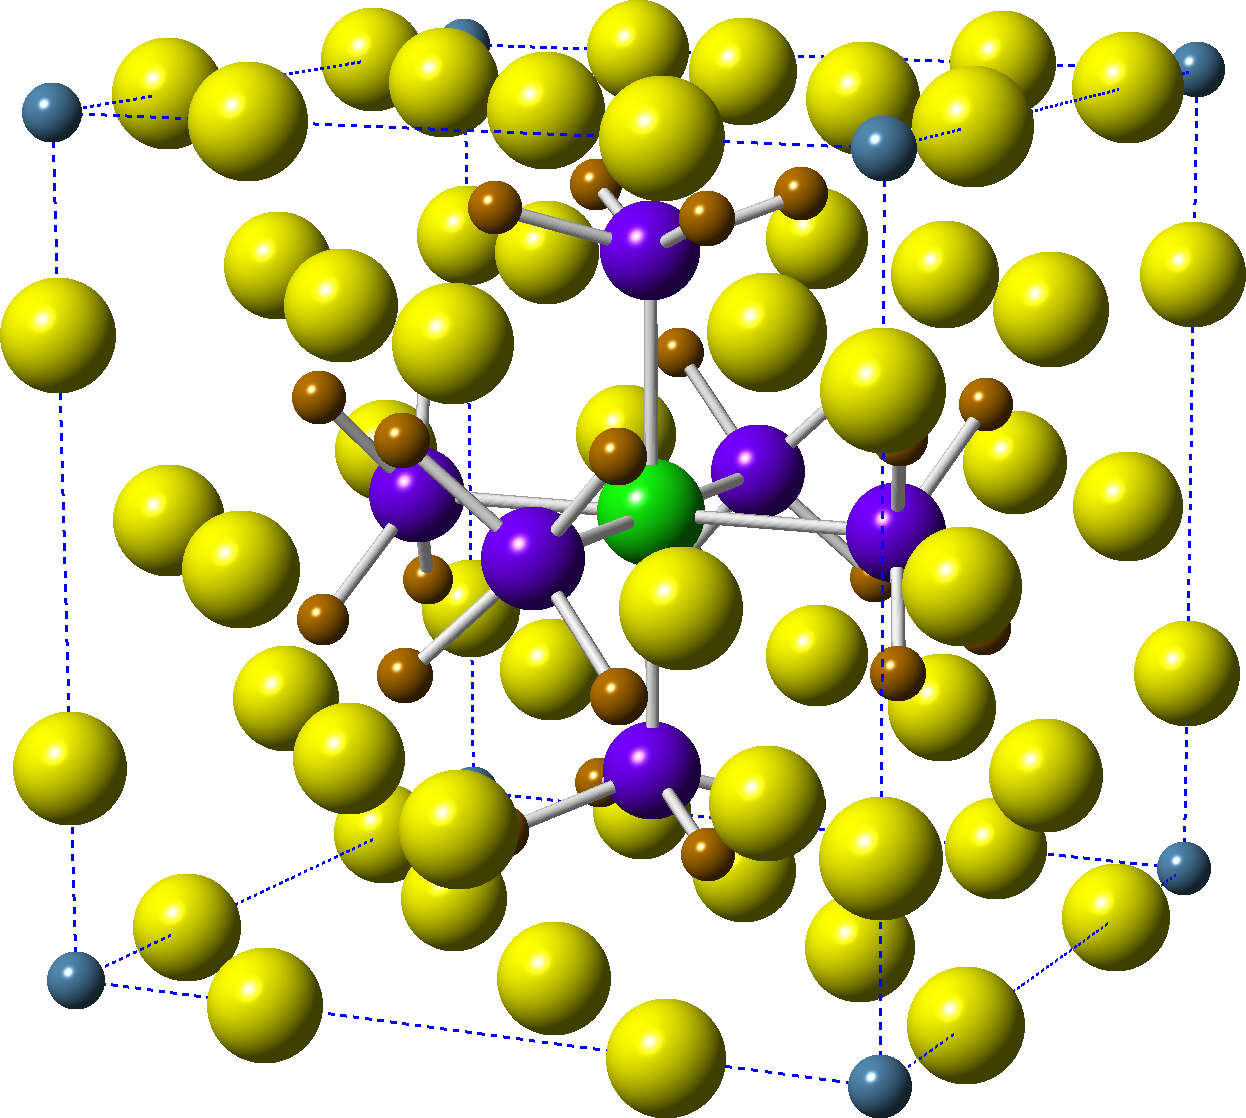
\includegraphics[height = 0.25\textwidth]{img/589-sol-2}}%
		{\caption{\texttt{0@a1,1@f1}($E = 0.0740$)}}
\end{subfloatrow}\\[0.5em]\begin{subfloatrow}
	\setlength{\columnsep}{1.5em}
	\ffigbox[0.32\textwidth]%
		{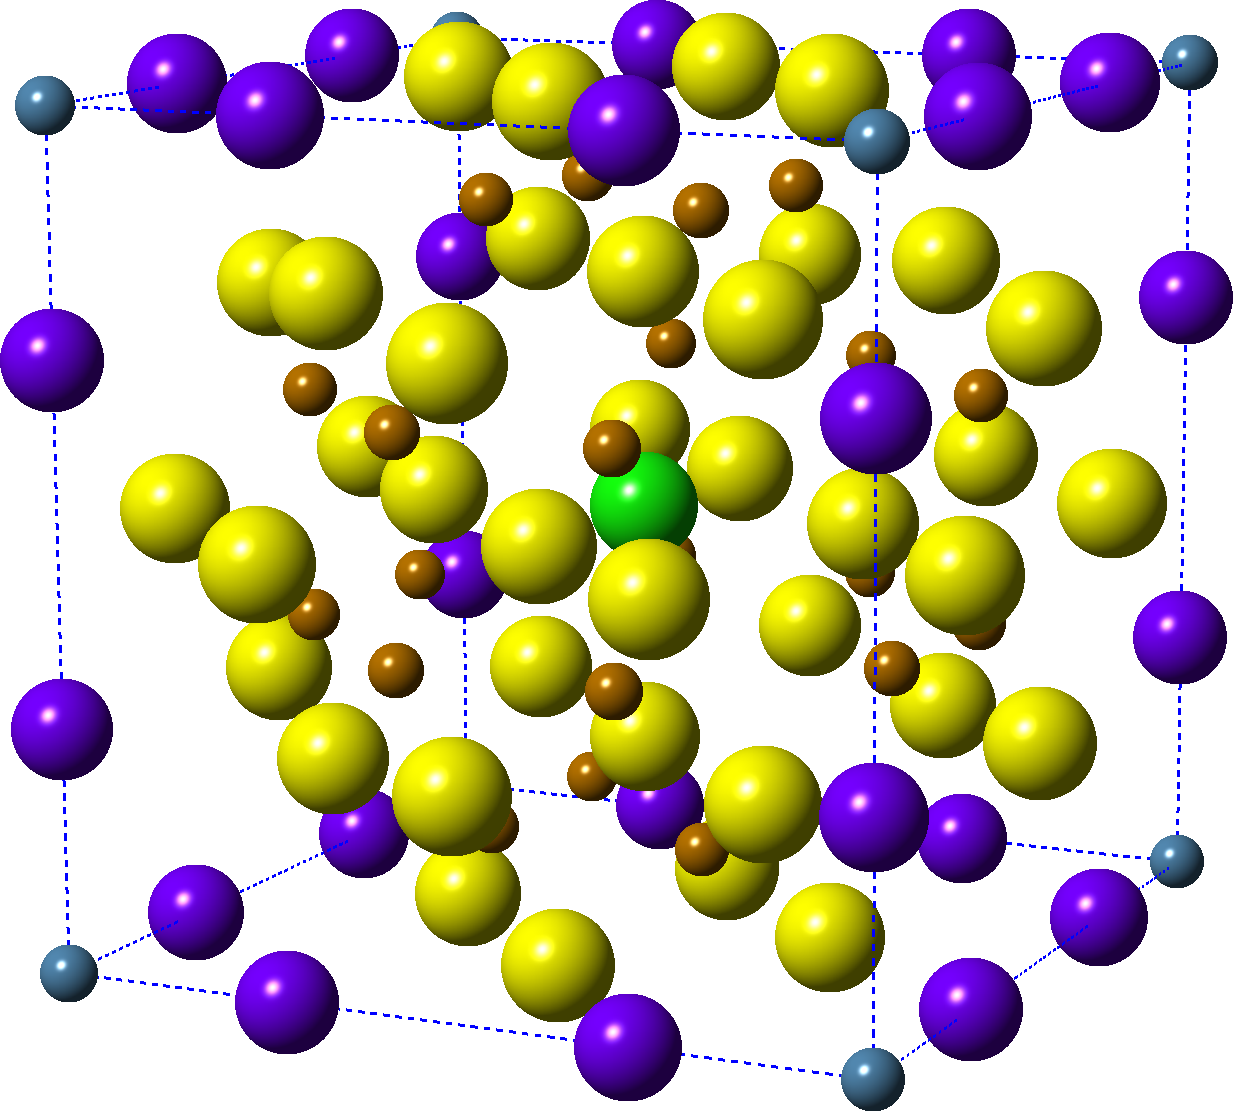
\includegraphics[height = 0.25\textwidth]{img/589-sol-3}}%
		{\caption{\texttt{0@a1,1@e1}($E = 0.0457$)}}
	\ffigbox[0.32\textwidth]%
		{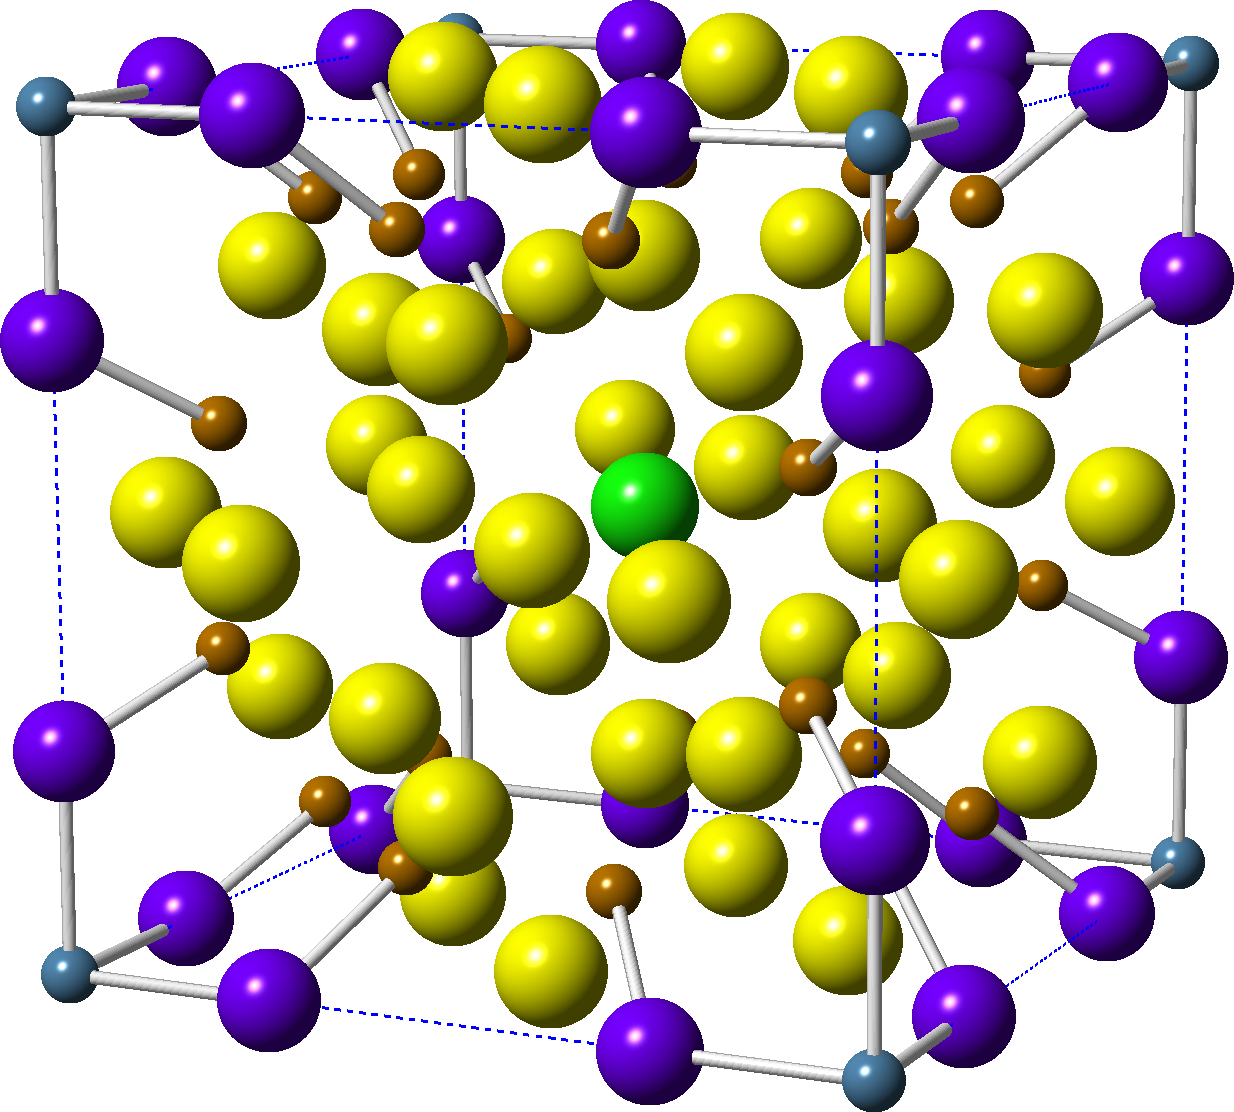
\includegraphics[height = 0.25\textwidth]{img/589-sol-4}}%
		{\caption{\texttt{0@a1,1@e1}($E = 0.0750$)}}
\end{subfloatrow}}{\caption[“0000589”的典型解]{%
	“0000589”的典型解(均已转换到使 \ce{Cl-} 在 $b$ 位置)%
}\label{fig:589-sol}}
\end{figure}

至此我们已经求解了 4 个测试结构。显然,如果只是手动输入(或复制、粘贴)第
\ref{ssec:decr-base} 小节中的命令并加以修改,这样会是十分低效且容易出错的。
在观察上述求解过程后,我们不难将其一般模式抽象为如下的 shell 脚本\footnote{%
	限于主题和篇幅,本文不试图对 shell 脚本编程进行详尽的解释;
	不熟悉相关背景的用户可以参考文献\parencite{robbins2005}。%
}(此处命名为 \verb|solve.sh|):
\begin{Verbatim}
\cm{#!/bin/sh}
decr_utils comb "$1" > combs.list
decr_utils dump "$1" < combs.list > crysts.list
decr_utils stat stat.sh hosts.conf < crysts.list > crysts.stat
decr_utils optim optim.sh hosts.conf < crysts.stat > crysts.optim
sort -k7g < crysts.optim > crysts.tmp && mv crysts.tmp crysts.optim
decr_utils merge "$1" < combs.list
\end{Verbatim}
这样只须将 \verb|hosts.conf| 复制到当前目录,便可通过以下命令求解:
\begin{Verbatim}
\cm{$} /path/to/solve.sh /path/to/some-cryst.txt
\end{Verbatim}
利用助手脚本(参考第 \ref{ssec:decr-arch} 小节)可以实现更加复杂的
自动化结构测定,相关内容将在第 \ref{sec:decr-adv} 节展示。

\subsection{EPC 筛选:以“0000428”和“0000219”结构为例}\label{ssec:epc-rank}

“0000428”结构($R\bar3$)的 decr 文件如下所示:
\begin{Verbatim}
\cm{# sg, abc, angles; ctl, extra; limits.}
148a	12.868 12.868 9.821	90 90 120
0.25 0.75 0.875	0.5 1.0
--

\cm{# rad/asf, n, limits, comb.}
Pb2+	18	--	--
Cr6+;Cr3+	3	--	--
O2-	24	--	--
Cl1-	18	--	--
\cm{# zooms.}
2:1-1

\cm{# 2theta, fwhm, hkl, mult, val.}
12.01	0.1	1 0 1	6	20.45
13.76	0.1	1 1 0	6	45.28
\cm{# (... further lines omitted ...)}
\end{Verbatim}
该结构的总 EPC 数为 88,单个 EPC 维数为 7--10,使用第 \ref{ssec:decr-auto} 小节
中的 \verb|solve.sh| 脚本求解时单次执行耗时约 \SI{25}{s}。虽然这个结构看似简单,
但是其求解并不十分直接,其中最重要的是直接使用 \verb|solve.sh| 时结果的重复性
出人意料地低:各 EPC 的排名并不稳定,且各 EPC 所得解的 $E$ 值浮动也较大;
根据本人的经验,这种情况通常是在维数大约为 15 的 EPC 中开始出现。无论如何,
在多次执行 \verb|solve.sh| 之后,不难发现排名最靠前的是以下 3 对等价 EPC%
($(0, 0, 1/2)$ 平移可使 $a/b$、$d/e$ 位置互变并保持其它 Wyckoff 记号不变):
\begin{itemize}
\item \verb|0@f1,1@a1,2@c1f1,3@f1|、\verb|0@f1,1@b1,2@c1f1,3@f1|:\\
	典型 $E$ 值为 0.057--0.060、0.064--0.066、0.075--0.100 或更大。
\item \verb|0@f1,1@a1,2@b1c2d1,3@f1|、\verb|0@f1,1@b1,2@a1c2e1,3@f1|:\\
	典型 $E$ 值为 0.097--0.099、0.103--0.121 或更大。
\item \verb|0@f1,1@a1,2@b1c2e1,3@f1|、\verb|0@f1,1@b1,2@a1c2d1,3@f1|:\\
	典型 $E$ 值为 0.113--0.114、0.120--0.125、0.162--0.168 或更大。
\end{itemize}
事实上,只须执行几次脚本便可注意到 \verb|1@a1,2@c1f1,...| 和
\verb|1@b1,2@c1f1,...| 所得解的最佳 $E$ 值明显低于其它两对 EPC,因此正确的
EPC 无疑是这一对。收集其各 $E$ 值的解,可发现 $E \geq 0.075$ 的解较为多样
(例如图 \ref{fig:428-sol}(c) 中的解),但 $E \in [0.064, 0.066]$ 的解(图
\ref{fig:428-sol}(b))和 $E \leq 0.060$ 的解(图 \ref{fig:428-sol}(a))基本
固定。考虑到后两个解从成键上看没有明显的问题,正确解应该是 $E$ 值最小的。

\begin{figure}[htbp!]\bfcmd
\ffigbox{\begin{subfloatrow}[3]
	\setlength{\columnsep}{-0.5em}
	\ffigbox[\FBwidth]{%
		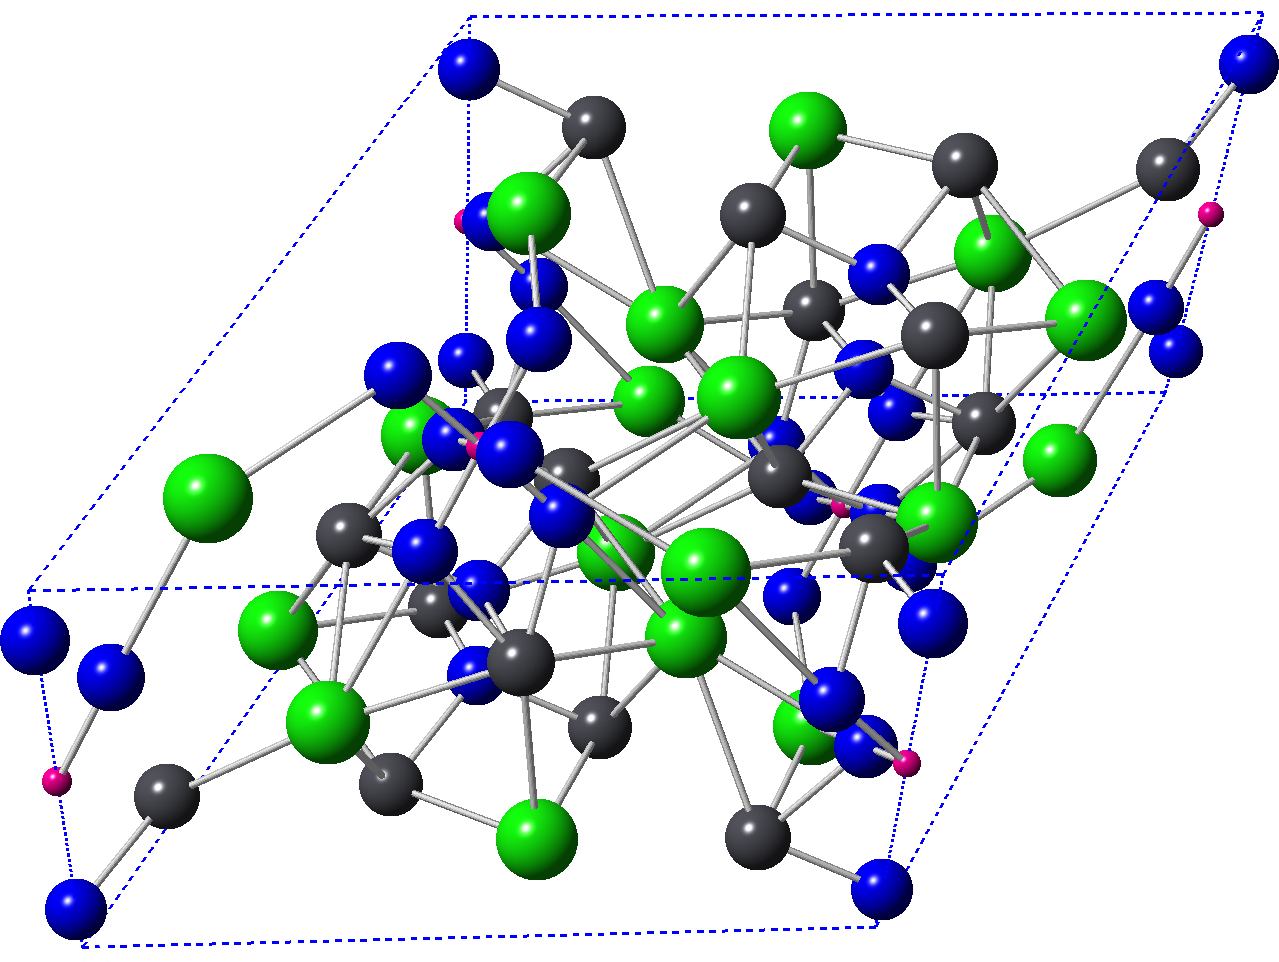
\includegraphics[width = 0.33\textwidth]{img/428-sol-1}%
	}{\caption{$R = 0.0586$}}
	\ffigbox[\FBwidth]{%
		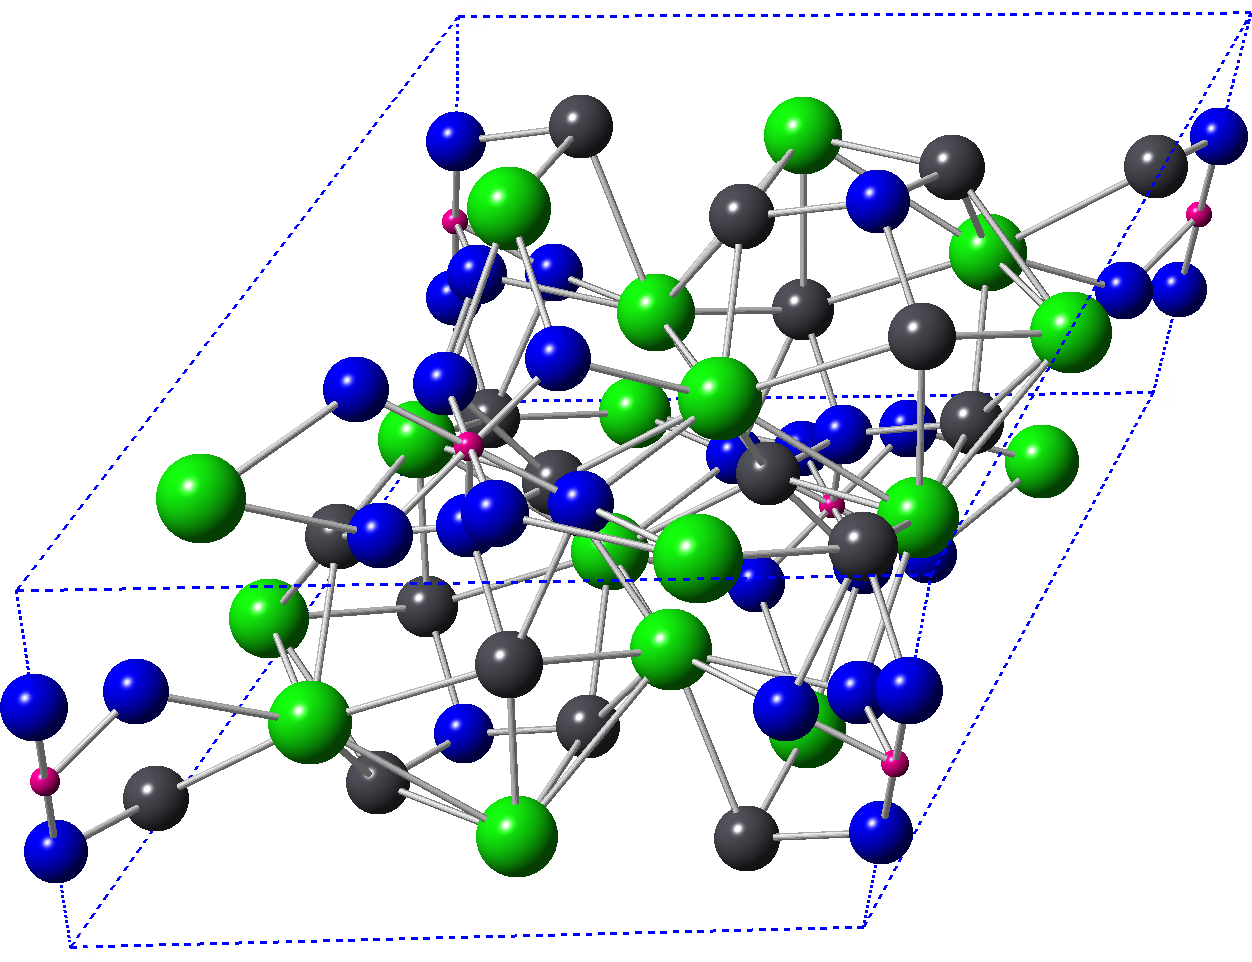
\includegraphics[width = 0.33\textwidth]{img/428-sol-2}%
	}{\caption{$R = 0.0650$}}
	\ffigbox[\FBwidth]{%
		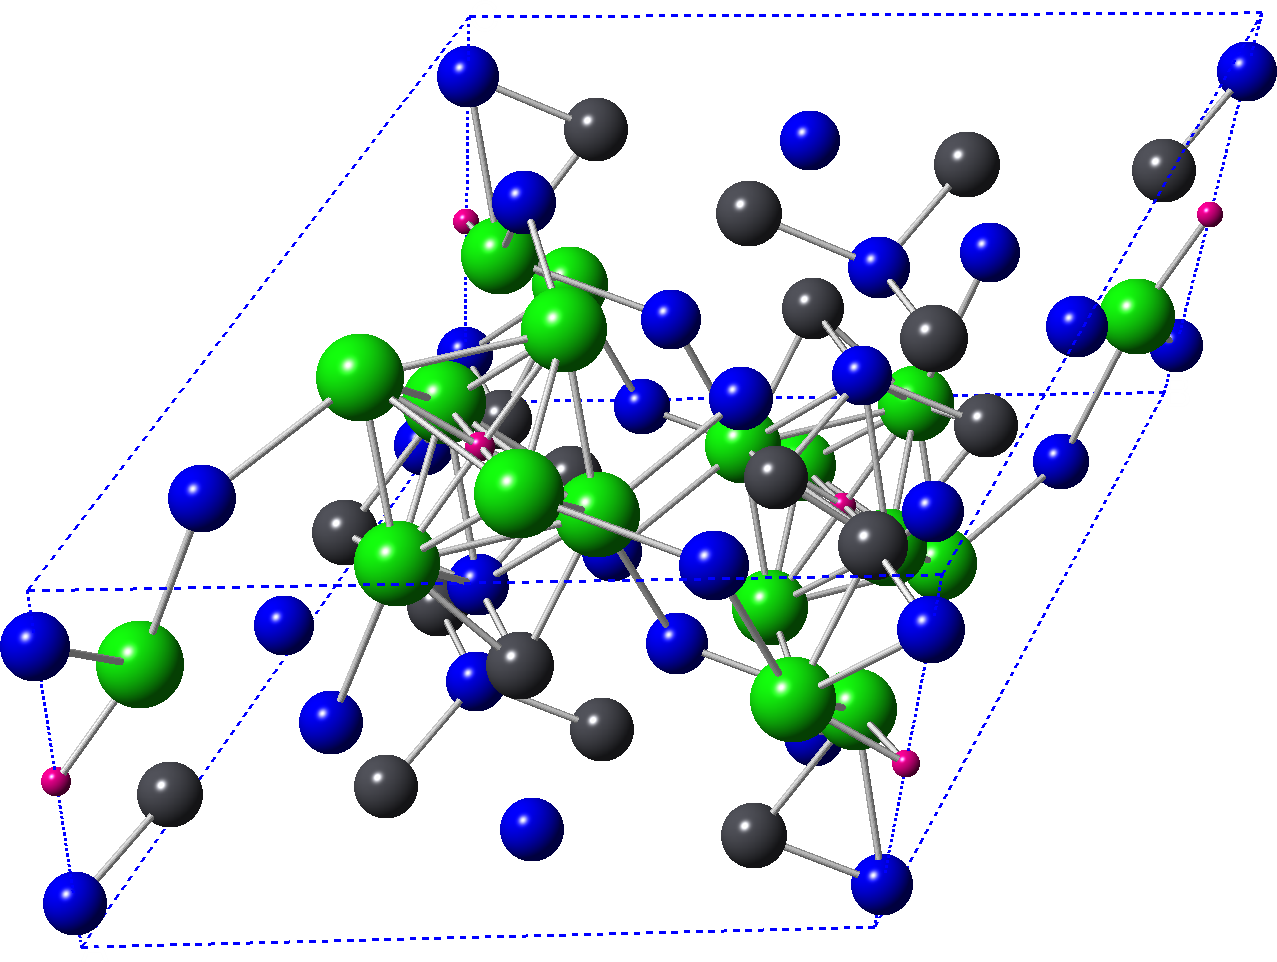
\includegraphics[width = 0.33\textwidth]{img/428-sol-3}%
	}{\caption{$R = 0.0801$}}
\end{subfloatrow}}{\caption[“0000428”的几个解]{%
	“0000428”的几个解,其中 (c) 只是相应 $E$ 值区间多种典型解中的一个%
}\label{fig:428-sol}}
\end{figure}

“0000219”结构(原数据采用的是 $Pbna$ 表示,求解前已转换\footnote{%
	可以使用 Bilbao 晶体学服务器\parencite{aroyo2006}上的 \texttt{SETSTRU}
	工具在同一空间群的不同表示之间转换,此外须特别注意 $hkl$ 和晶胞参数都需要
	转换。顺便值得一提的是,用此工具还可以对独立原子的 Wyckoff 位置进行判断,
	从而方便计算测试结构的晶胞化学式,以及寻找独立原子在 \emph{decryst}
	所用不对称单元内等效原子的坐标。%
}到 $Pbcn$)的 decr 文件如下所示:
\begin{Verbatim}
\cm{# sg, abc, angles; ctl, extra; limits.}
60	8.536 9.404 9.973	90 90 90
0.25 0.75 0.875	0.5 1.0
--

\cm{# rad/asf, n, limits, comb.}
P5+;P	8	--	--
Fe3+	12	--	--
O2-	44	--	--
\cm{# zooms.}
2:0-0	1.2:1-1	1.5:0-1

\cm{# 2theta, fwhm, hkl, mult, val.}
14.01	0.1	1 1 0	4	3.05
16.61	0.1	1 1 1	8	18.09
\cm{# (... further lines omitted ...)}
\end{Verbatim}
容易发现,原封不动地使用上述 \verb|solve.sh| 脚本求解须花费很长时间(约
\SI{1.5}{\hour}),这不难理解:观察 \verb|crysts.list| 可见虽然总 EPC
数不大(284),但是单个 EPC 的维数并不低(14--23),这导致每个 EPC
(特别是那些接近或超过 20 维的)须要花费很长的时间来求解。在这样的
情况下,我们可以根据统计分析的结果对 EPC 进行筛选:中断求解\footnote{%
	EPC 的维数对统计分析耗时的影响较小,因此我们来得及获取统计分析的结果。%
},并执行以下命令
\begin{Verbatim}
\cm{$} awk '\lb{} print 1 " " (1 / $7 + 10 * $6 / $5) "\bs{}t" $0 \rb{}' \bs
	< crysts.stat > crysts.rank0
\end{Verbatim}
来根据 \emph{EPCryst}\parencite{deng2011}中使用的经验公式计算各 EPC
的品质因数(FOM)。观察 \verb|crysts.rank0| 可发现各 EPC 的 FOM
并没有非常明显的聚类现象,因此我们先尝试对前 $1/4$ 的 EPC 求解:
\begin{Verbatim}
\cm{$} sed 70q < crysts.rank0 | cut -f 2-3 > crysts.stat
\cm{$} decr_utils optim optim.sh hosts.conf < crysts.stat > crysts.optim
\cm{$} sort -k7g < crysts.optim > crysts.tmp && mv crysts.tmp crysts.optim
\cm{$} decr_utils merge /path/to/0000219.txt < combs.list
\end{Verbatim}
观察 \verb|crysts.optim|,可见最佳 EPC 通常大致如下(注意 $(0, 1/2, 0)$
平移可使 $Pbcn$ 空间群中 $a/b$ 位置互变并保持其它 Wyckoff 记号不变):
\begin{Verbatim}
\cm{>} [...] 0.637264 0.0639186 0.0296934	0@d1,1@a1d1,2@c1d5.cr
\cm{>} [...] 0.638173 0.0653523 0.0484107	0@d1,1@b1d1,2@c1d5.cr
\cm{>} [...] 0.637305 0.0693133 0.0834741	0@d1,1@c1d1,2@b1d5.cr
\cm{>} [...] 0.638933 0.0675984 0.0847271	0@d1,1@c1d1,2@a1d5.cr
\cm{>} ...
\end{Verbatim}
于是可知只有 \verb|0@d1,1@a1d1,2@c1d5|、\verb|0@d1,1@b1d1,2@c1d5| 这对等价
EPC 是正确的;在可视化软件中查看 $E$ 值为 0.0297 和 0.0484 的两个解模型(图
\ref{fig:219-sol}),可见后者主要是部分 \ce{O^{2-}} 原子在 $c$ 方向上发生了
违背成键规律的较大偏移。加入以上 EPC 筛选之后,求解所需时长可以压缩到约
\SI{45}{\minute}(只压缩了约 $1/2$ 的时间,因为筛选出的 EPC 多为 18--22 维)。

\begin{figure}[htbp!]\bfcmd
\ffigbox{\begin{subfloatrow}
	\setlength{\columnsep}{2em}
	\ffigbox[\FBwidth]%
		{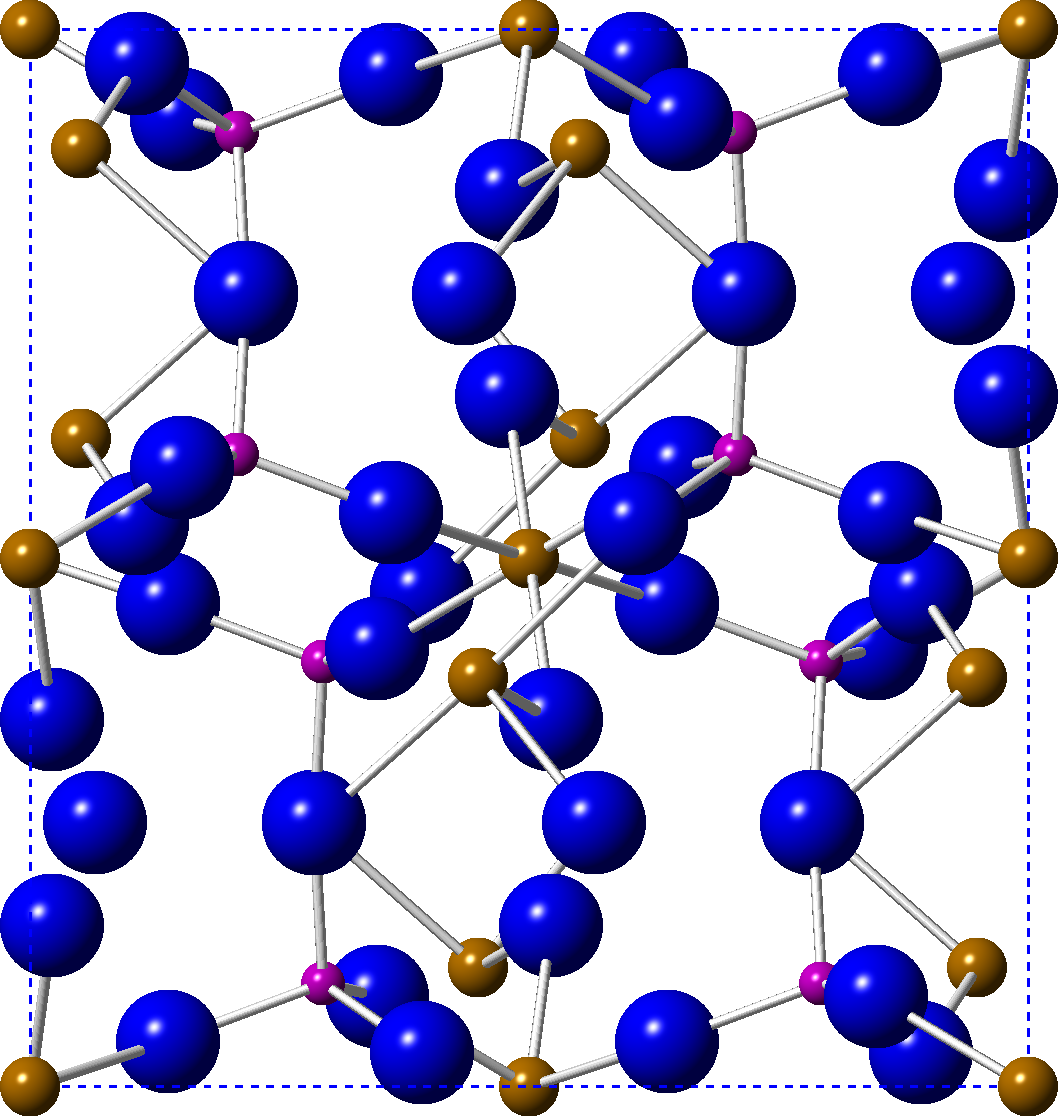
\includegraphics[width = 0.25\textwidth]{img/219-sol-1}}%
		{\caption{$E = 0.0297$}}
	\ffigbox[\FBwidth]%
		{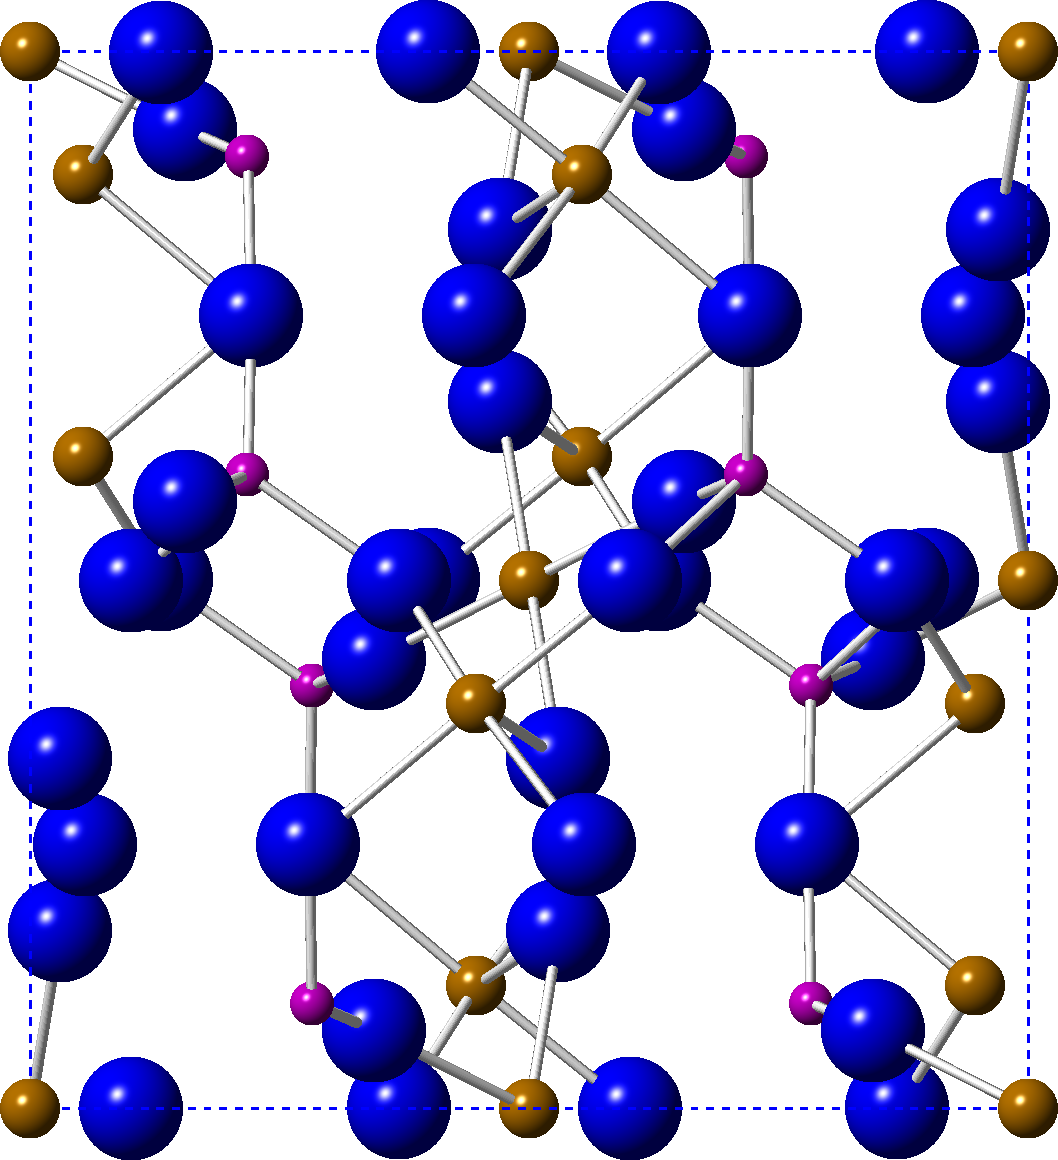
\includegraphics[width = 0.25\textwidth]{img/219-sol-2}}%
		{\caption{$E = 0.0484$}}
\end{subfloatrow}}{\caption[“0000219”典型解在 $a$ 方向上的投影]{%
	“0000219”典型解在 $a$ 方向上的投影
	(均已转换到使部分 \ce{Fe^{3+}} 在 $a$ 位置)%
}\label{fig:219-sol}}
\end{figure}

这里有必要强调,本章所有求解均是在启用了 Intel i7-3720QM CPU 的所有 8 个处理器
线程的前提下进行的:在求解其它结构时这或许不是必需,但在求解“0000219”时可以
看到,因为 EPC 任务是完美并行的(参考第 \ref{ssec:decr-para} 小节),所以我们
利用并行节省了大约 $0.75 \times 7 = \SI{5.2}{\hour}$ 的时间,这是不可忽视的。
可能有读者会疑惑,在硬件性能突飞猛进的当代,从软件方面提升计算效率是否仍有
必要?事实上,根据近年来 CPU 性能的增长趋势(图 \ref{fig:fp-perf}),%
CPU 的单线程浮点性能大约是每 12 年提升一个数量级,所以数倍的性能提升
仍然具有重要意义,何况在单线程性能增长放缓的背景之下大力发展
并行和分布式计算本来就是科学计算(乃至通用计算)的大势所趋。

\begin{figure}[htbp!]
\ffigbox{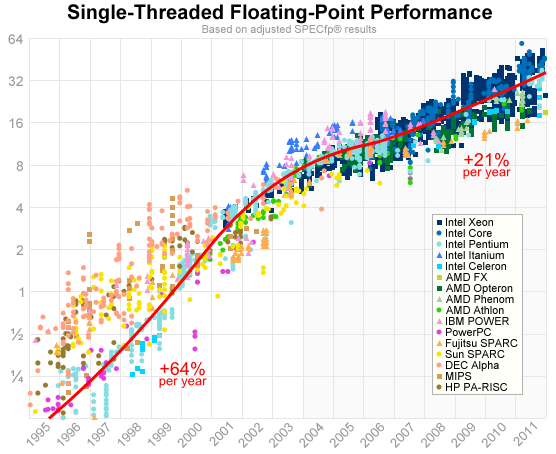
\includegraphics[width = 0.75\textwidth]{img/fp-perf}}{\caption[%
	CPU 单线程浮点性能在 1995--2011 年间的增长%
]{%
	CPU 单线程浮点性能在 1995--2011 年间的增长
	(图引自文献 (\cite{preshing2012}))%
}\label{fig:fp-perf}}
\end{figure}

\section{\emph{decryst} 的高级用法和常用技巧}\label{sec:decr-adv}

在本节中,第 \ref{ssec:heavy-atom} 小节将演示如何利用 \emph{decryst} 的自动化
机制实现正空间法中的重原子法,而重原子法是之后各小节中结构测定的基础。第
\ref{ssec:epc-search} 小节将演示如何实现对重原子、轻原子等效点系组合(EPC)
的分步确定,以及在此之后如何自动化地对同时涉及轻、重原子的 EPC 进行准确的求解。
第 \ref{ssec:epc-filter} 小节将演示对 EPC 的复杂筛选:其中不仅会用到之前的
EPC 筛选方法,而且会在结构测定的各个步骤中多次利用原子重叠评估函数(参考第
\ref{ssec:eval-func} 小节)对 EPC 进行精细的筛选。

\subsection{重原子法:以 \ce{PbSO4} 为例}\label{ssec:heavy-atom}

\ce{PbSO4}(原数据采用的是 $Pbnm$ 表示,求解前已转换到 $Pnma$)的
decr 文件(假设文件名为 \verb|pso.txt|)如下所示:
\begin{Verbatim}
\cm{# sg, abc, angles; ctl, extra; limits.}
62	8.4720 5.3973 6.9549	90 90 90
0.25 0.75 0.875	0.5 1.0
--

\cm{# rad/asf, n, limits, comb.}
Pb2+	4	--	--
S6+;S	4	--	--
O2-	16	--	--
\cm{# zooms.}
1.4:1-0	2.8:1-1
0.9:2-1

\cm{# 2theta, fwhm, hkl, mult, val.}
16.49	0.2	1 0 1	4	2.70
20.83	0.2	0 1 1	4	79.73
\cm{# (... further lines omitted ...)}
\end{Verbatim}

\ce{PbSO4} 结构可以直接使用第 \ref{ssec:decr-auto} 小节中的 \verb|solve.sh|
脚本求解,耗时约 \SI{8}{\second};然而考虑到 \ce{PbSO4} 中 \ce{Pb^{2+}} 和
\ce{S^{6+}} 均明显地重于 \ce{O^{2-}},该结构的简单性使其在演示重原子法时
成为一个完美的例子。为了使用重原子法求解 \ce{PbSO4} 结构,我们首先须要使
\emph{decryst} 忽略 \ce{O^{2-}} 原子,这可以通过注释实现:
\begin{Verbatim}
\cm{$} sed -i '/^O2-/ s/^/#/; /:2-/ s/^/#/' pso.txt
\end{Verbatim}
注意原 \verb|decr| 文件中以 \verb|O2-| 开头的行只有指定晶胞中 \ce{O^{2-}}
个数的行,且该文件中包含 \verb|2:| 字符串的数据行只有指定和 \ce{O^{2-}}
相关对缩放因子的行,因此以上命令能够精准地注释掉所有涉及 \ce{O^{2-}}
的数据行。由于重原子法须要分步求解重、轻原子,为了避免不同步骤中的
文件互相覆盖,我们可以在不同目录中生成不同步骤所需的文件:
\begin{Verbatim}
\cm{$} mkdir ps
\cm{$} decr_utils comb pso.txt | awk '\lb print "ps/pso," $0 \rb' |
	decr_utils dump pso.txt > ps/index.list
\end{Verbatim}

在 \verb|ps| 目录中生成 cryst 文件和 crysts 文件之后,
便可以对各 EPC 进行统计分析和全局最优化:
\begin{Verbatim}
\cm{$} PYTHONUNBUFFERED=1 decr_utils stat stat.sh hosts.conf < ps/index.list |
	tee ps/index.tmp | do_rank.sh 0 > ps/index.rank0
\cm{$} grep -v '^#' < ps/index.rank0 | cut -f 2-3 |
	PYTHONUNBUFFERED=1 decr_utils optim optim.sh hosts.conf |
	tee ps/index.tmp | do_rank.sh 1 > ps/index.rank1
\end{Verbatim}
\verb|PYTHONUNBUFFERED| 环境变量强制 Python 将每一行结果分别输出而不是将若干行
结果凑到一起输出。助手脚本 \verb|do_rank.sh| 的作用是在 crysts 文件中添加两列
以记录各 EPC 的品质因数(FOM,基于 \emph{EPCryst}\parencite{deng2011}%
中的经验公式)以及是否零维,例如以下数据行(为了方便解释,
此处明确区分了代码中的空格和制表符)
\begin{Verbatim}[showtabs = true, showspaces = true]
\cm{>\ }0 0 - - - - 0.522904	ps/pso,0@b1,1@a1.cr
\cm{>\ }2 1000 200 0.01 0.396994 0.140564 0.129636	ps/pso,0@c1,1@a1.cr
\end{Verbatim}
将被变换为
\begin{Verbatim}[showtabs = true, showspaces = true]
\cm{>\ }0 3.82479	... - - 0.522904	ps/pso,0@b1,1@a1.cr
\cm{>\ }1 11.2546	... 0.396994 0.140564 0.129636	ps/pso,0@c1,1@a1.cr
\end{Verbatim}
\verb|do_rank.sh| 的命令行参数决定了其对数据行排序的方式:为 \verb|1| 时
只根据 FOM 排序,而为 \verb|0| 时将零维 EPC 排在前面,然后才是按 FOM 排序。
注意其中使用 \verb|grep| 命令去掉了 \verb|index.rank0| 中用“\verb|#|”
注释掉的行,从而避免对这些行计算上述的临时字段。此外,以上操作中
有规律地使用了空白字符(参考第 \ref{ssec:decr-fmt} 小节),
从而方便了之后使用 \verb|cut| 命令去掉上述临时字段;
这一技巧事实上已经在第 \ref{ssec:decr-auto} 小节中使用。

在求解完重原子的坐标之后,我们就可以导出结果了:
\begin{Verbatim}
\cm{$} do_filter.sh < ps/index.rank1 | decr_utils merge pso.txt > /dev/null
\end{Verbatim}
\verb|decr_utils| 在导出 decr 文件时会保留原有注释,
于是上一步中 \verb|pso.txt| 的片段
\begin{Verbatim}
\cm{#O2-}	\cm{16}	\cm{--}	\cm{--}
\cm{# Pairwise zoom factors.}
1.4:1-0 2.8:1-1
\cm{#0.9:2-1}
\end{Verbatim}
在正确 EPC 所对应的 decr 文件(\verb|ps/pso,0@c1,1@c1.cr|)中将被变换为
\begin{Verbatim}
\cm{#O2-}	\cm{16}	\cm{--}	\cm{--}
\cm{# Pairwise zoom factors.}
1.4:1-0 2.8:1-1
\cm{#0.9:2-1}
0@c1	0.314226	0.25	0.33363
1@c1	0.43269	0.25	0.805449
\end{Verbatim}
因此为了求解 \ce{O^{2-}} 原子的位置,我们只须去掉所有涉及 \ce{O^{2-}} 的注释:
\begin{Verbatim}
\cm{$} sed -i '/^#O2-/ s/^#//; /:2-/ s/^#//' pso.txt
\cm{$} do_filter.sh < ps/index.rank1 | sed 's/\bs.cr$/.txt/' |
	xargs -n 100 sed -i '/^#O2-/ s/^#//; /:2-/ s/^#//'
\end{Verbatim}
其中 \verb|do_filter.sh| 的作用是提取 \verb|rank|
文件中未被注释的 cryst 文件名,例如
\begin{Verbatim}
\cm{> #0 3.82479}	\cm{... - - 0.522904}	\cm{ps/pso,0@b1,1@a1.cr}
\cm{>} 1 11.2546	... 0.396994 0.140564 0.129636	ps/pso,0@c1,1@a1.cr
\end{Verbatim}
将被变换为
\begin{Verbatim}
\cm{>} ps/pso,0@c1,1@a1.cr
\end{Verbatim}

接下来我们须要产生 \ce{O^{2-}} 原子的 EPC:
\begin{Verbatim}
\cm{$} mkdir pso
\cm{$} do_filter.sh < ps/index.rank1 | sed 's/\bs.cr$/.txt/' | while read f; do
	decr_utils comb "$f" | awk '\lb
	     print "pso/'"$(basename $f | sed -r 's@\bs.[^/.]+$@,@')"'" $0
	\rb' | decr_utils dump "$f" >> pso/index.list; done
\end{Verbatim}
以上第 2 行命令的作用是将从重原子 EPC 所对应 decr 文件生成的 cryst 文件冠以
相应重原子 EPC 的前缀:例如从 \verb|ps/pso,0@c1,1@c1.txt| 生成的 \verb|2@c1d1|
cryst 文件将被保存到 \verb|pso/pso,0@c1,1@c1,2@c1d1.cr|;通过这一操作,
我们事实上得到了(包含所有原子的)总 EPC 的完整表达式。\ce{O^{2-}}
原子的统计分析和全局最优化步骤和之前如出一辙,不再赘述:
\begin{Verbatim}
\cm{$} PYTHONUNBUFFERED=1 decr_utils stat stat.sh hosts.conf < pso/index.list |
	tee pso/index.tmp | do_rank.sh 0 > pso/index.rank0
\cm{$} grep -v '^#' < pso/index.rank0 | cut -f 2-3 |
	PYTHONUNBUFFERED=1 decr_utils optim optim.sh hosts.conf |
	tee pso/index.tmp | do_rank.sh 1 > pso/index.rank1
\cm{$} do_filter.sh < pso/index.rank1 | decr_utils merge pso.txt > /dev/null
\cm{$} rm ps/index.tmp pso/index.tmp
\end{Verbatim}
除去人工步骤之后,以上求解过程总耗时约 \SI{5}{\second}。

\subsection{实际 EPC 的搜索:以“0000158”结构为例}\label{ssec:epc-search}

第 \ref{ssec:heavy-atom} 小节中求解 \ce{PbSO4} 结构所用的命令行操作具有很强的
典型性:许多代码在其它结构的求解中只需很少修改就可以使用,这些代码被抽象为了
助手脚本;在使用助手脚本之后,\ce{PbSO4} 结构的求解可以用以下脚本实现:
\begin{Verbatim}
\cm{#!/bin/sh}
sed -i '/^O2-/ s/^/#/; /:2-/ s/^/#/' pso.txt
mkdir ps
echo pso.txt | do_dump.sh ps
do_stat.sh ps && do_optim.sh ps && do_merge.sh pso.txt ps
sed -i '/^#O2-/ s/^#//; /:2-/ s/^#//' pso.txt
do_filter.sh < ps/index.rank1 | sed 's/\bs.cr$/.txt/' |
	xargs -n 100 sed -i '/^#O2-/ s/^#//; /:2-/ s/^#//'
mkdir pso
do_filter.sh < ps/index.rank1 | sed 's/\bs.cr$/.txt/' | do_dump.sh pso
do_stat.sh pso && do_optim.sh pso && do_merge.sh pso.txt pso
rm ps/index.tmp pso/index.tmp
\end{Verbatim}
可能有读者会感到疑惑:脚本一般是用于自动化地运行具有重复性的任务,但晶体
结构在解出之后一般不用重复求解,那么这样的求解脚本有什么意义?事实上,
因为实际结构的求解往往是相当复杂的,其步骤和参数往往需要多次调整;因此,
求解脚本不仅可以方便用户在调整求解步骤和参数时对求解的全程进行宏观的把握,
而且可以作为增强求解过程可重复性的“实验记录”,从而为其它结构的求解提供参考。
事实上,本节中后两种结构的求解都是以上述 \ce{PbSO4} 求解脚本为基础的。

“0000158”结构($C2/c$)的 decr 文件(假设文件名为 \verb|158.txt|)如下所示:
\begin{Verbatim}
\cm{# sg, abc, angles; ctl, extra; limits.}
15a	10.129 8.306 8.533	90 112.19 90
0.25 0.75 0.875	0.5 1.0
--

\cm{# rad/asf, n, limits, comb.}
Ca2+	4	--	--
S6+;S	8	--	--
Na1+	8	--	--
O2-	32	--	--
\cm{# zooms.}
2.8:1-1
1.2:2,0-1

\cm{# 2theta, fwhm, hkl, mult, val.}
14.24	0.1	1 1 0	4	44.67
18.92	0.1	2 0 0	2	23.65
\cm{# (... further lines omitted ...)}
\end{Verbatim}
该结构的总 EPC 数为 3706,单个 EPC 维数为 9--19;注意到其中的原子可以分为重原子
\ce{S^{6+}}、\ce{Ca^{2+}} 和轻原子 \ce{Na+}、\ce{O^{2-}},其可以使用重原子法
求解以节约时间,因此我们首先求解重原子(EPC 数为 44,单个 EPC 维数为 0--4):
\begin{Verbatim}
\cm{$} sed -ri '/^(O2-|Na1\bs+)/ s/^/#/; /:2,/ s/^/#/' 158.txt
\cm{$} mkdir cs
\cm{$} echo 158.txt | do_dump.sh cs
\cm{$} do_stat.sh cs && do_optim.sh cs && do_merge.sh 158.txt cs
\end{Verbatim}

观察 \verb|cs/index.rank1|,不难注意到 \verb|0@e1,1@f1| 是唯一合理的重原子 EPC:
其 $E$ 值为 0.20 左右,其它非零维 EPC 的 $E$ 值都在 0.30--0.40 之间,而所有零维
EPC 的 $E$ 值都大于 0.40。因此我们在求解轻原子时只采用 \verb|0@e1,1@f1|
这一重原子 EPC(下属 EPC 数为 350,单个 EPC 维数为 6--15):
\begin{Verbatim}
\cm{$} sed -i '2,$ s/^/#/' cs/index.rank1
\cm{$} sed -ri '/^#(O2-|Na1\bs+)/ s/^#//; /:2,/ s/^#//' 158.txt
\cm{$} do_filter.sh < cs/index.rank1 | sed 's/\bs.cr$/.txt/' |
	xargs -n 100 sed -ri '/^#(O2-|Na1\bs+)/ s/^#//; /:2,/ s/^#//'
\cm{$} mkdir no
\cm{$} do_filter.sh < cs/index.rank1 | sed 's/\bs.cr$/.txt/' | do_dump.sh no
\cm{$} do_stat.sh no && do_optim.sh no && do_merge.sh 158.txt no
\end{Verbatim}
观察 \verb|no/index.rank1| 可见各 EPC 的 $E$ 值没有明显的聚类现象,所以求解似乎
失败了,但事实并非如此:在“0000158”中,重原子 \ce{S^{6+}}、\ce{Ca^{2+}} 和轻原子
\ce{Na+}、\ce{O^{2-}} 的电子数相差并不悬殊,因此对重、轻原子分别求解得不到很满意
的结果并不难理解。然而从直觉上不难理解分别求解得到的(包含所有原子的)总 EPC
排名和直接对所有原子求解得到的总 EPC 排名仍会存在一定的相关性,因此我们可以对
排名靠前的总 EPC 再次进行求解(这里取了前 30 个;此外注意 \verb|do_dump.sh| 生成
的 cryst 文件名包含了总 EPC 的完整表达式,参考第 \ref{ssec:heavy-atom} 小节):
\begin{Verbatim}
\cm{$} sed -i '31,$ s/^/#/' no/index.rank1
\cm{$} mkdir csno
\cm{$} do_filter.sh < no/index.rank1 | sed 's@^[^,]\bs+,@@; s/\bs.cr//' |
	awk '\lb print "csno/158," $0 ".cr\bs{}t" $0 \rb' |
	decr_utils dump 158.txt > csno/index.list
\cm{$} do_stat.sh csno && do_optim.sh csno && do_merge.sh 158.txt csno
\end{Verbatim}

观察 \verb|csno/index.rank1| 可见正确 EPC \verb|0@e1,1@f1,2@f1,3@f4| 是
唯一合理的 EPC:其 $E$ 值最多为 0.05 左右,而其它 EPC 的 $E$ 值都至少为 0.13
左右。注意到该 EPC 的维数为 19,我们须要多次进行全局最优化,然后挑选最优解:
\begin{Verbatim}
\cm{$} mkdir fin
\cm{$} l="$(sed 1q < csno/index.rank1 | sed 's/csno/fin/; s/\.cr$//')"
\cm{$} name="$(echo "$l" | cut -f 3 | sed 's@.*/@@')"
\cm{$} for i in $(seq 0 9); do
	cp csno/"$name".cr fin/"$name-$i".cr
	echo "$l-$i".cr >> fin/index.rank0; done
\cm{$} do_optim.sh fin && do_merge.sh 158.txt fin
\cm{$} rm */index.tmp
\end{Verbatim}
\verb|fin/index.rank1| 中排名最靠前的一般会是 3 个左右的 $E$ 值在 0.025--0.030
的解,这些就是正确解;除去人工步骤之后,以上求解过程总耗时约 \SI{5}{\minute}。

\subsection{EPC 的复杂筛选:以“0009563”结构为例}\label{ssec:epc-filter}

“0009563”结构($P\bar3c1$)的 decr 文件(假设文件名为 \verb|0009563.txt|)
如下所示(为了方便解释,此处明确区分了代码中的空格和制表符):
\begin{Verbatim}[showtabs = true, showspaces = true]
\cm{# sg, abc, angles; ctl, extra; limits.}
165	12.19 12.19 10.14	90 90 120
0.25 0.75 0.875	0.5 1.0
--

\cm{# rad/asf, n, limits, comb.}
Rb1+	12	--	--
Ge4+	18	--	--
Ti4+	6	--	--
O2-	54	--	--
\cm{# zooms.}
1.5:1,2-1,2

\cm{# 2theta, fwhm, hkl, mult, val.}
16.97	0.2	1 1 1	12	10.71
17.49	0.2	0 0 2	2	7.14
\cm{# (... further lines omitted ...)}
\end{Verbatim}
本小节的详细测试结果(包括图 \ref{fig:9563-sol} 所对应的结构数据)可以从文献%
\parencite{liu2018}的补充材料中获取。注意到“0009563”中的金属原子均明显重于
\ce{O^{2-}},使用重原子法求解是很合适的,因此本人首先生成了重原子的
cryst 文件(EPC 数为 1451 个,单个 EPC 维数为 5--8):
\begin{Verbatim}
\cm{$} mkdir rgt-0
\cm{$} sed '/^O2-/ s/^/#/; s/^0\bs.25 /0.99 /' < 0009563.txt > 9563.txt
\cm{$} echo 9563.txt | do_dump.sh rgt-0
\cm{$} mkdir rgt-1
\cm{$} sed -i 's/^0\bs.99 /0.25 /' 9563.txt
\cm{$} echo 9563.txt | do_dump.sh rgt-1
\end{Verbatim}
因为 EPC 数很大,我们须要尽量对其进行筛选,从而减少(包含所有原子的)总 EPC
备选范围。受\textcite{lu1965},\textcite{reddy1965}所做工作的启发,本人生成了
两套 cryst 文件,其中组合因子 $\mu$(参考第 \ref{ssec:decr-fmt} 小节)
的值分别为\footnote{%
	考虑到部分化学上很不合理的 EPC 可能以大概率产生原子重叠评估函数值 $B = 1$
	的晶体模型,不将 $\mu$ 值设定为 1 可以避免这些 EPC 的全局最优化过早结束。%
} 0.99 和默认的 0.25;通过对 $\mu = 0.99$ 的 cryst 文件进行全局最优化,
我们就可以筛除那些不可能产生无原子重叠晶体模型的 EPC。此外还须要强调的是
\verb|0009563.txt| 中在行首出现且后面跟着空格的数值只有 $\mu$ 值,
这是以上命令可以精准地对 $\mu$ 值进行更改的基础。

我们接下来会看到,即使事先筛除不可能产生无原子重叠晶体模型的 EPC,全局最优化
仍可能得到发生重叠的解模型;为了筛除这种解模型,本人定义了一个在 crysts
文件中加入原子重叠评估函数值 $B$ 的 shell 函数:
\begin{Verbatim}
\cm{$} do_bump_sh() \lb
	while read l; do
	name="$(echo "$l" | cut -f 3 | sed 's/\bs.cr$/.txt/')"
	echo 'nil.cr nil' | decr_utils dump "$name" > /dev/null
	sed 's/0\bs.25 0\bs.75 0\bs.875$/0.99 0.75 0.875/' < nil.cr |
	     decr_mcs 0 | cut -d ' ' -f 3 | tr '\bs{}n' ' '
	echo "$l"; done; \rb
\end{Verbatim}
其中 \verb|nil| EPC 的意义可以参考第 \ref{ssec:decr-fmt} 小节。接下来本人
按照上文所述的思路对之前产生的 cryst 文件进行了统计分析和全局最优化:
\begin{Verbatim}
\cm{$} do_stat.sh rgt-0 && do_optim.sh rgt-0
\cm{$} mv -f rgt-0/index.rank1 rgt-0/index.tmp
\cm{$} awk '\lb print ($9 > 0.12 ? "#" : "") $0 \rb' \bs
	< rgt-0/index.tmp > rgt-0/index.rank1
\cm{$} do_filter.sh < rgt-0/index.rank1 | sed 's@.*/@rgt-1/@' > rgt-1/index.tmp
\cm{$} grep -Ff rgt-1/index.tmp < rgt-1/index.list > rgt-1/index.tmpp
\cm{$} mv -f rgt-1/index.tmpp rgt-1/index.list
\cm{$} do_stat.sh rgt-1 && do_optim.sh rgt-1 && do_merge.sh 9563.txt rgt-1
\cm{$} do_bump_sh < rgt-1/index.rank1 | awk '\lb print
	($10 > 0.2 || $1 > 0.02 ? "#" : "") $0 \rb' > rgt-1/index.rank2
\end{Verbatim}
以上命令先筛除了 $\mu = 0.99$ 时解模型 $E > 0.12$ 的 EPC,剩下 183 个(13\%);
在恢复默认 $\mu$ 值后又筛除了解模型 $E > 0.2$ 的 EPC,剩下 26 个。本人在观察
\verb|index.rank2| 之后发现其中的 EPC 分为一组解模型 $B \leq 0.0027$ 的和一组
解模型 $B \in [0.056, 0.112]$ 的,并由此筛除了所有解模型 $B > 0.02$ 的 EPC,
剩下 20 个(11\%)。除去人工步骤之后,重原子 EPC 求解耗时约 \SI{2.5}{\minute}。
事实上,重原子求解得到了正确的结果:正确 EPC \verb|0@g1,1@f1g1,2@b1d1| 的
$E$ 值(0.058)是最小的;事后本人在可视化软件中查看重原子 EPC 的解模型,
确认了所有因 $B$ 值过大而被筛除的解模型中都发生了很明显的原子重叠。

仿照以上步骤,本人对 \ce{O^{2-}} 原子的 EPC 进行了求解:
\begin{Verbatim}
\cm{$} mkdir rgto-0 && sed -i '/^#O2-/ s/^#//; s/^0\bs.25 /0.99 /' 9563.txt
\cm{$} do_filter.sh < rgt-1/index.rank2 | sed 's/\bs.cr$/.txt/' |
	xargs -n 100 sed -i '/^#O2-/ s/^#//; s/^0\bs.25 /0.99 /'
\cm{$} do_filter.sh < rgt-1/index.rank2 |
	sed 's/\bs.cr$/.txt/' | do_dump.sh rgto-0
\cm{$} mkdir rgto-1 && sed -i 's/^0\bs.99 /0.25 /' 9563.txt
\cm{$} do_filter.sh < rgt-1/index.rank2 | sed 's/\bs.cr$/.txt/' |
	xargs -n 100 sed -i 's/^0\bs.99 /0.25 /'
\cm{$} do_filter.sh < rgt-1/index.rank2 |
	sed 's/\bs.cr$/.txt/' | do_dump.sh rgto-1
\cm{$} do_stat.sh rgto-0 && mv -f rgto-0/index.rank0 rgto-0/index.tmp
\cm{$} awk '\lb print ($9 > 0.99 ? "#" : "") $0 \rb' \bs
	< rgto-0/index.tmp > rgto-0/index.rank0
\cm{$} do_optim.sh rgto-0 && mv -f rgto-0/index.rank1 rgto-0/index.tmp
\cm{$} awk '\lb print ($9 > 0.05 ? "#" : "") $0 \rb' \bs
	< rgto-0/index.tmp > rgto-0/index.rank1
\cm{$} do_filter.sh < rgto-0/index.rank1 |
	sed 's@.*/@rgto-1/@' > rgto-1/index.tmp
\cm{$} grep -Ff rgto-1/index.tmp < rgto-1/index.list > rgto-1/index.tmpp
\cm{$} mv -f rgto-1/index.tmpp rgto-1/index.list
\cm{$} do_stat.sh rgto-1 && do_optim.sh rgto-1 && do_merge.sh 9563.txt rgto-1
\cm{$} do_bump_sh < rgto-1/index.rank1 |
	awk '\lb print ($1 > 0.02 ? "#" : "") $0 \rb' > rgto-1/index.rank2
\end{Verbatim}
在这一步骤中,本人首先基于之前筛选得到的重原子 EPC 生成了 \ce{O^{2-}} 的 EPC(共
4455 个,维数主要为 10--13)。在筛除不可能产生无原子重叠晶体模型的 EPC 时为了
节省时间,本人先在统计分析后筛除了 $E$ 的最佳值大于 0.99 的 EPC,剩下 2186 个
(49\%);在全局最优化之后又筛除了解模型 $E > 0.05$ 的 EPC,剩下 110 个(5\%)。

考虑到 \ce{O^{2-}} 对“0009563”的衍射谱影响有限,而其 EPC 维数较高,我们可以逐步
缩小备选 EPC 的范围。在上一步骤中,本人已经筛除了解模型 $B > 0.02$ 的 EPC,
剩下 50 个;接下来,本人又重复进行了 2 次全局最优化,
并分别选取了 $E$ 值排名前 20 和前 10 的 EPC:
\begin{Verbatim}
\cm{$} i=0; for n in 21 11; do
	[ "$i" -eq 0 ] && c=rgto-1/index.rank2 ||
	     c=fin-$((i - 1))/index.rank1
	d=fin-"$i"; mkdir "$d"
	do_filter.sh < "$c" | sed 's@.*/@rgto-1/@' > "$d"/index.tmp
	grep -Ff "$d"/index.tmp < rgto-1/index.rank0 |
	     sed 's/rgto-1/'"$d"'/' > "$d"/index.rank0
	cp $(cat "$d"/index.tmp) "$d" && do_optim.sh "$d"
	sed -i "$n"',$ s/^/#/' "$d"/index.rank1
	do_merge.sh 9563.txt "$d"; i=$((i + 1)); done
\end{Verbatim}
事后本人观察上述步骤中产生的 \verb|index.rank1| 文件,确认了这 10 个 EPC
通常都是在其中排名靠前的。本人对这些 EPC 中的每一个进行了 10 次全局最优化,
并筛除了所得解模型中 $B > 0.02$ 的那些,最后剩下了 90 个解模型:
\begin{Verbatim}
\cm{$} c="$d"/index.rank1; d=fin-"$i"; mkdir "$d"
\cm{$} do_filter.sh < "$c" | sed 's@.*/@rgto-1/@' > "$d"/index.tmp
\cm{$} grep -Ff "$d"/index.tmp < rgto-1/index.rank0 |
	sed 's/rgto-1/'"$d"'/' > "$d"/index.list
\cm{$} cat "$d"/index.list | while read l; do
	name="$(echo "$l" | sed 's@.*/@@; s/\bs.cr$//')"
	l="$(echo "$l" | cut -f 1-2)"; for i in $(seq 0 9); do
	     cp rgto-1/"$name".cr "$d"/"$name-$i".cr
	     printf '%s\bs{}t%s\bs{}n' "$l" "$d"/"$name-$i".cr >> "$d"/index.rank0
	done; done
\cm{$} do_optim.sh "$d" && do_merge.sh 9563.txt "$d"
\cm{$} do_bump_sh < "$d"/index.rank1 |
	awk '\lb print ($1 > 0.02 ? "#" : "") $0 \rb' > "$d"/index.rank2
\cm{$} rm -f 9563.txt nil.cr */index.tmp
\end{Verbatim}
除去人工步骤之后,\ce{O^{2-}}原子 EPC 的求解耗时约 \SI{25}{\minute}。本人首先按
EPC 分组查看了上述的 90 个解,发现除正确 EPC \verb|0@g1,1@f1g1,2@b1d1,3@f1g4|
之外的 EPC 生成的解在成键关系上都有明显的问题:难以解释的不均匀配位数(图
\ref{fig:9563-sol}(c)),有孤立 \ce{O^{2-}} 的前提下金属原子被金属原子配位
(图 \ref{fig:9563-sol}(d)),等等。又考虑到这一 EPC 产生了上述 100 个解中排名
最靠前的 10 个,其无疑是“0009563”唯一合理的 EPC;在这 10 个解中,本人找到了 2
种互不等价的合理解:一种(图 \ref{fig:9563-sol}(a))和数据库中的记录基本一致,
其原子坐标只需轻微的精修;另一种(图 \ref{fig:9563-sol}(b))一眼看去没有明显的
问题,但事实上可以注意到其中 \ce{Ge^{4+}} 原子的配位多面体有很明显的畸变。

\begin{figure}[!htbp]
\floatsetup{heightadjust = none}
\captionsetup{justification = centering}
\ffigbox{\begin{subfloatrow}
	\setlength{\columnsep}{1.5em}
	\ffigbox[0.4\textwidth]{%
		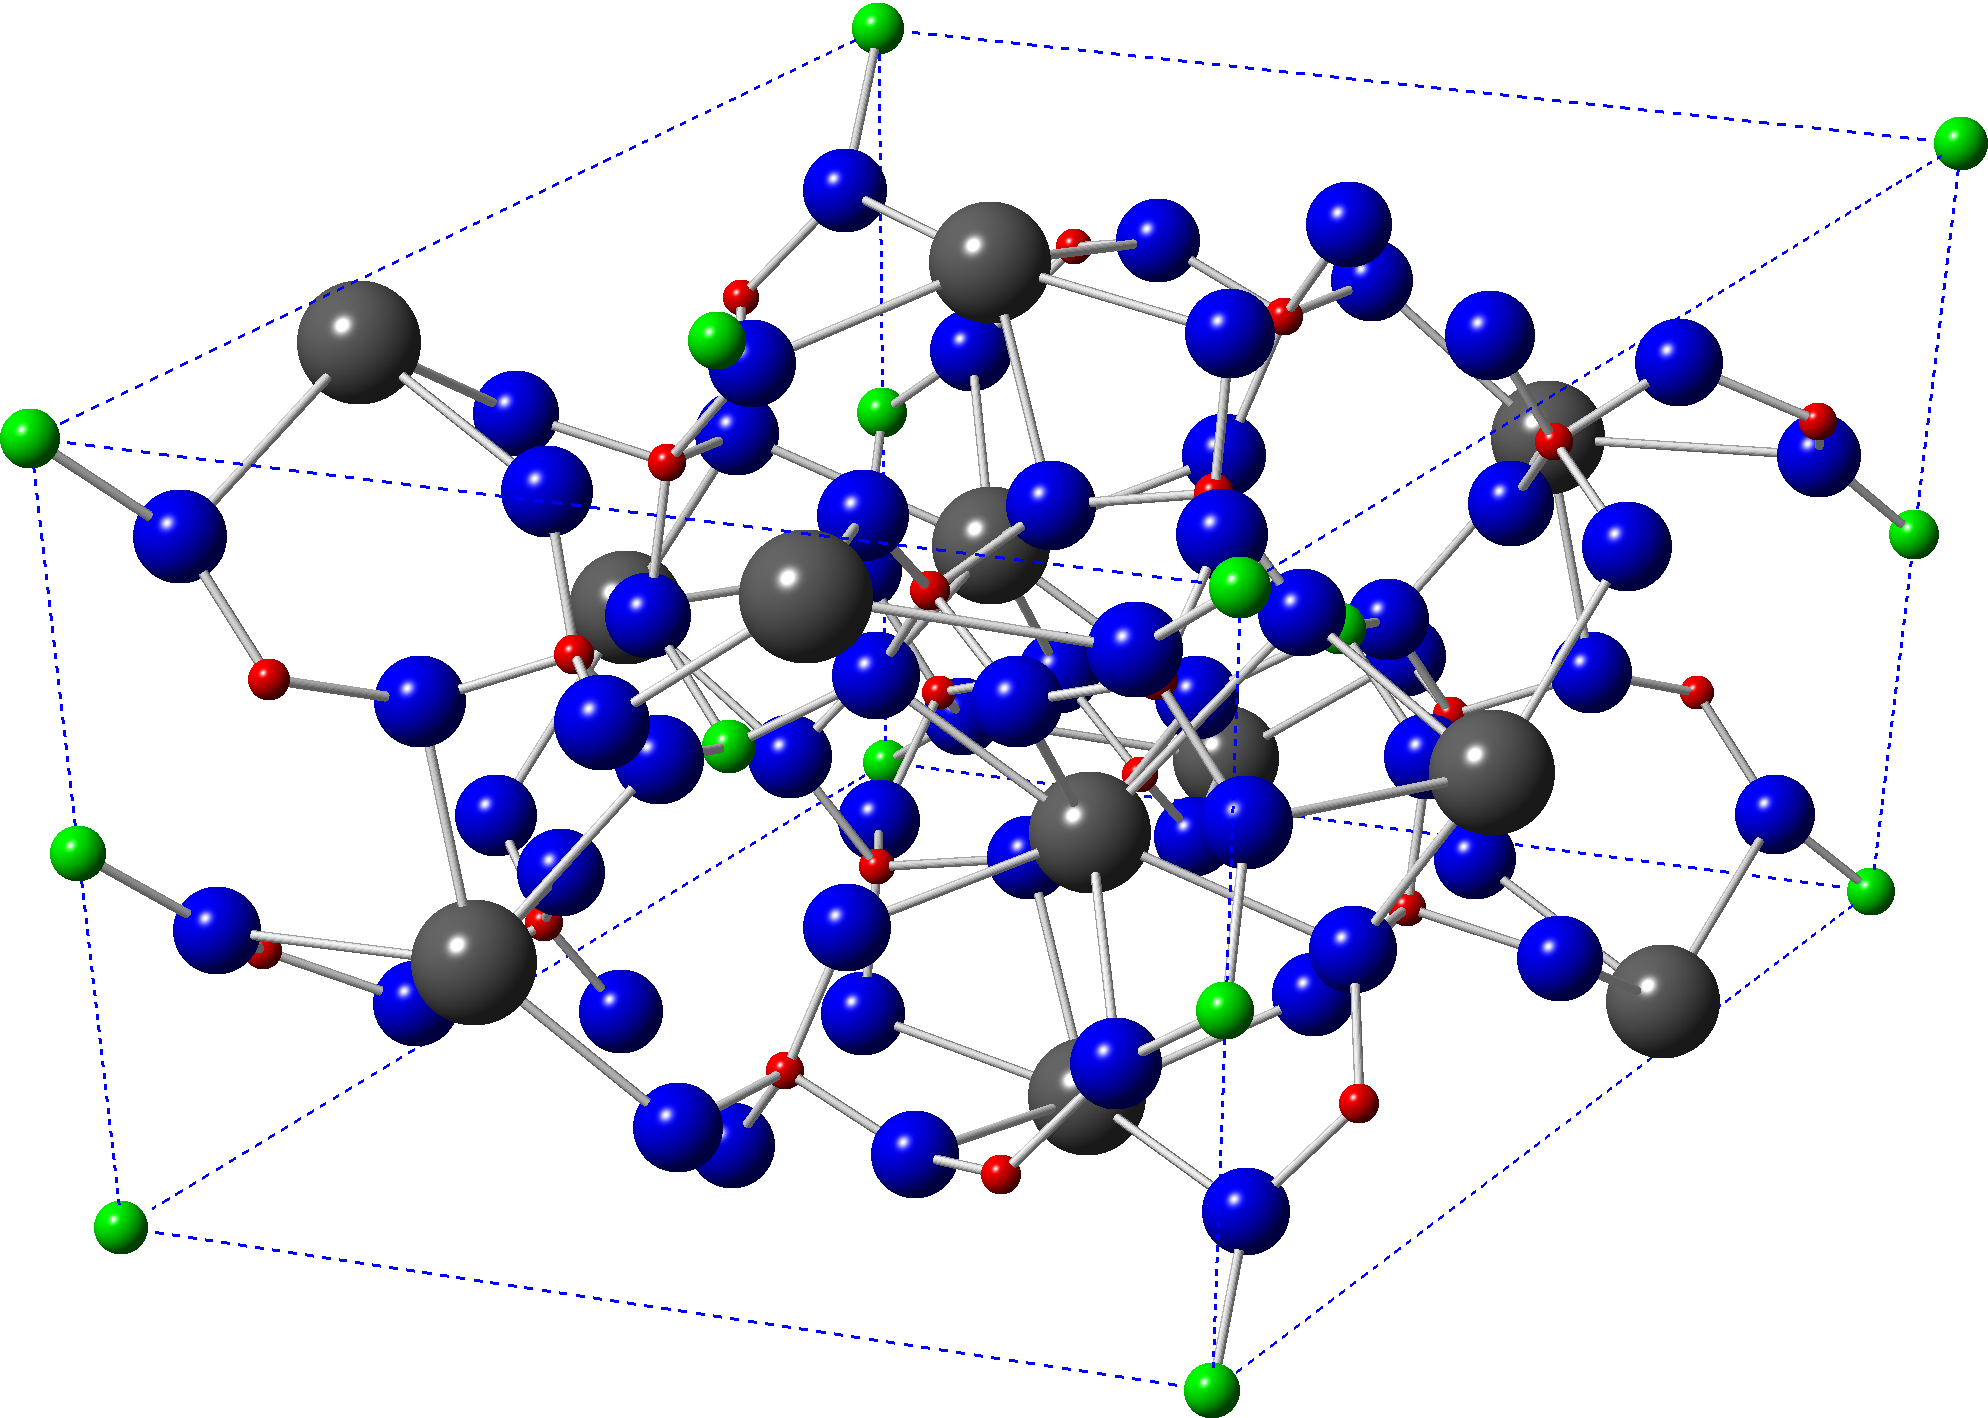
\includegraphics[height = 0.27\textwidth]{img/rgto-sol-1}
	}{\caption{%
		\texttt{0@g1,1@f1g1,2@b1d1,3@f1g4}\\(正确解)%
	}}
	\ffigbox[0.4\textwidth]{%
		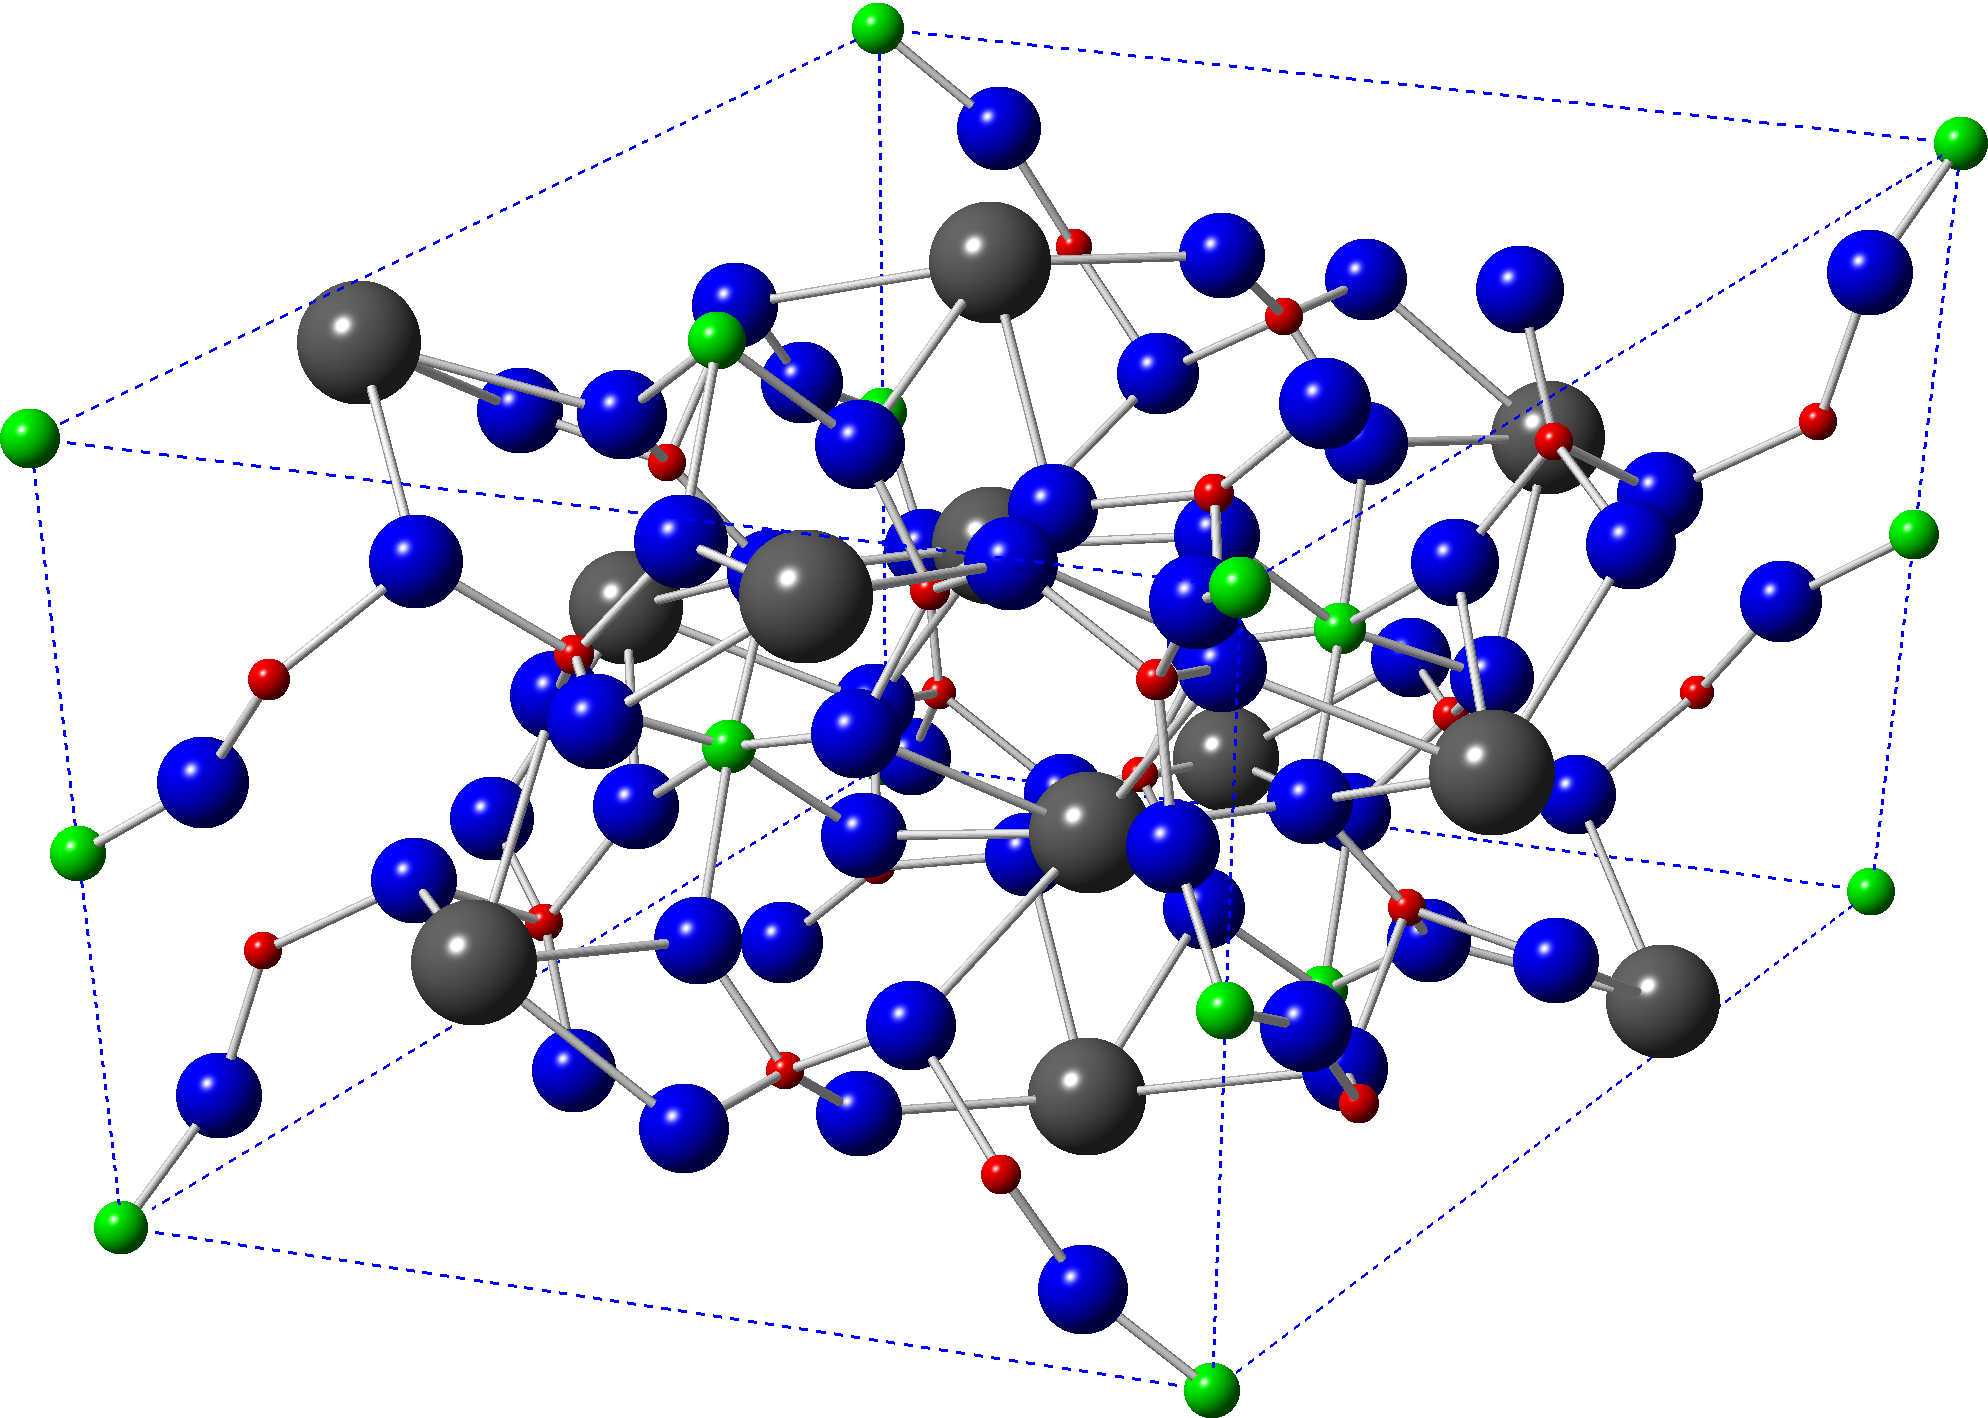
\includegraphics[height = 0.27\textwidth]{img/rgto-sol-2}%
	}{\caption{%
		\texttt{0@g1,1@f1g1,2@b1d1,3@f1g4}\\(\ce{Ge^{4+}} 配位多面体畸变严重)%
	}}
\end{subfloatrow}\\[0.4em]\begin{subfloatrow}
	\setlength{\columnsep}{1.5em}
	\ffigbox[0.4\textwidth]{%
		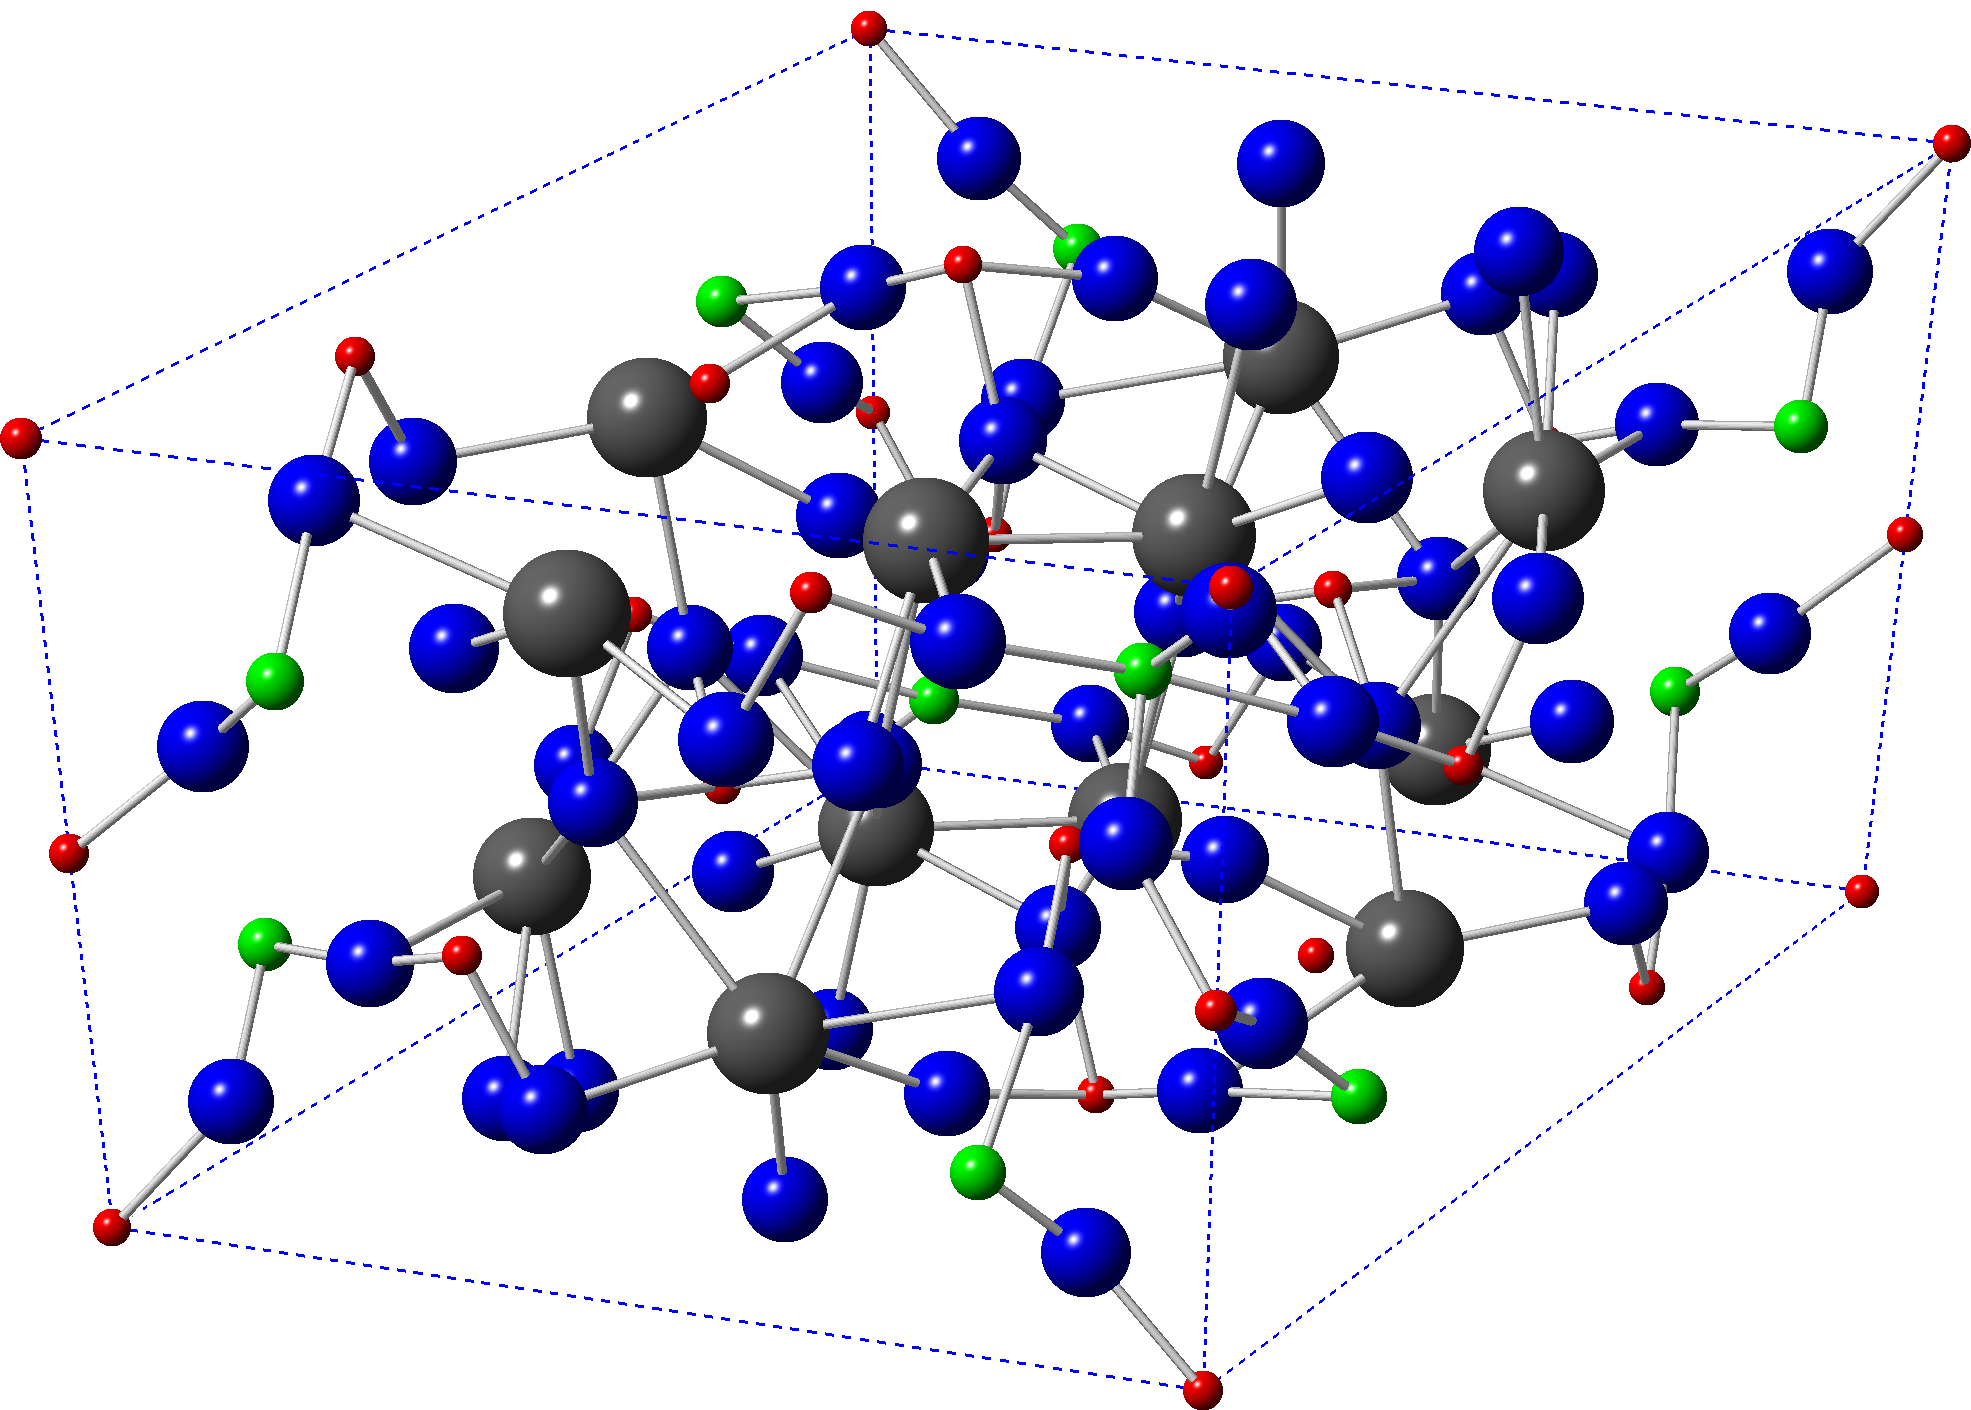
\includegraphics[height = 0.27\textwidth]{img/rgto-sol-3}%
	}{\caption{%
		\texttt{0@g1,1@b1d1g1,2@f1,3@f1g4}\\($b$ 位置的
		\ce{Ge^{4+}} 为 6 配位,\\其它位置的 \ce{Ge^{4+}} 为 3 配位)%
	}}
	\ffigbox[0.4\textwidth]{%
		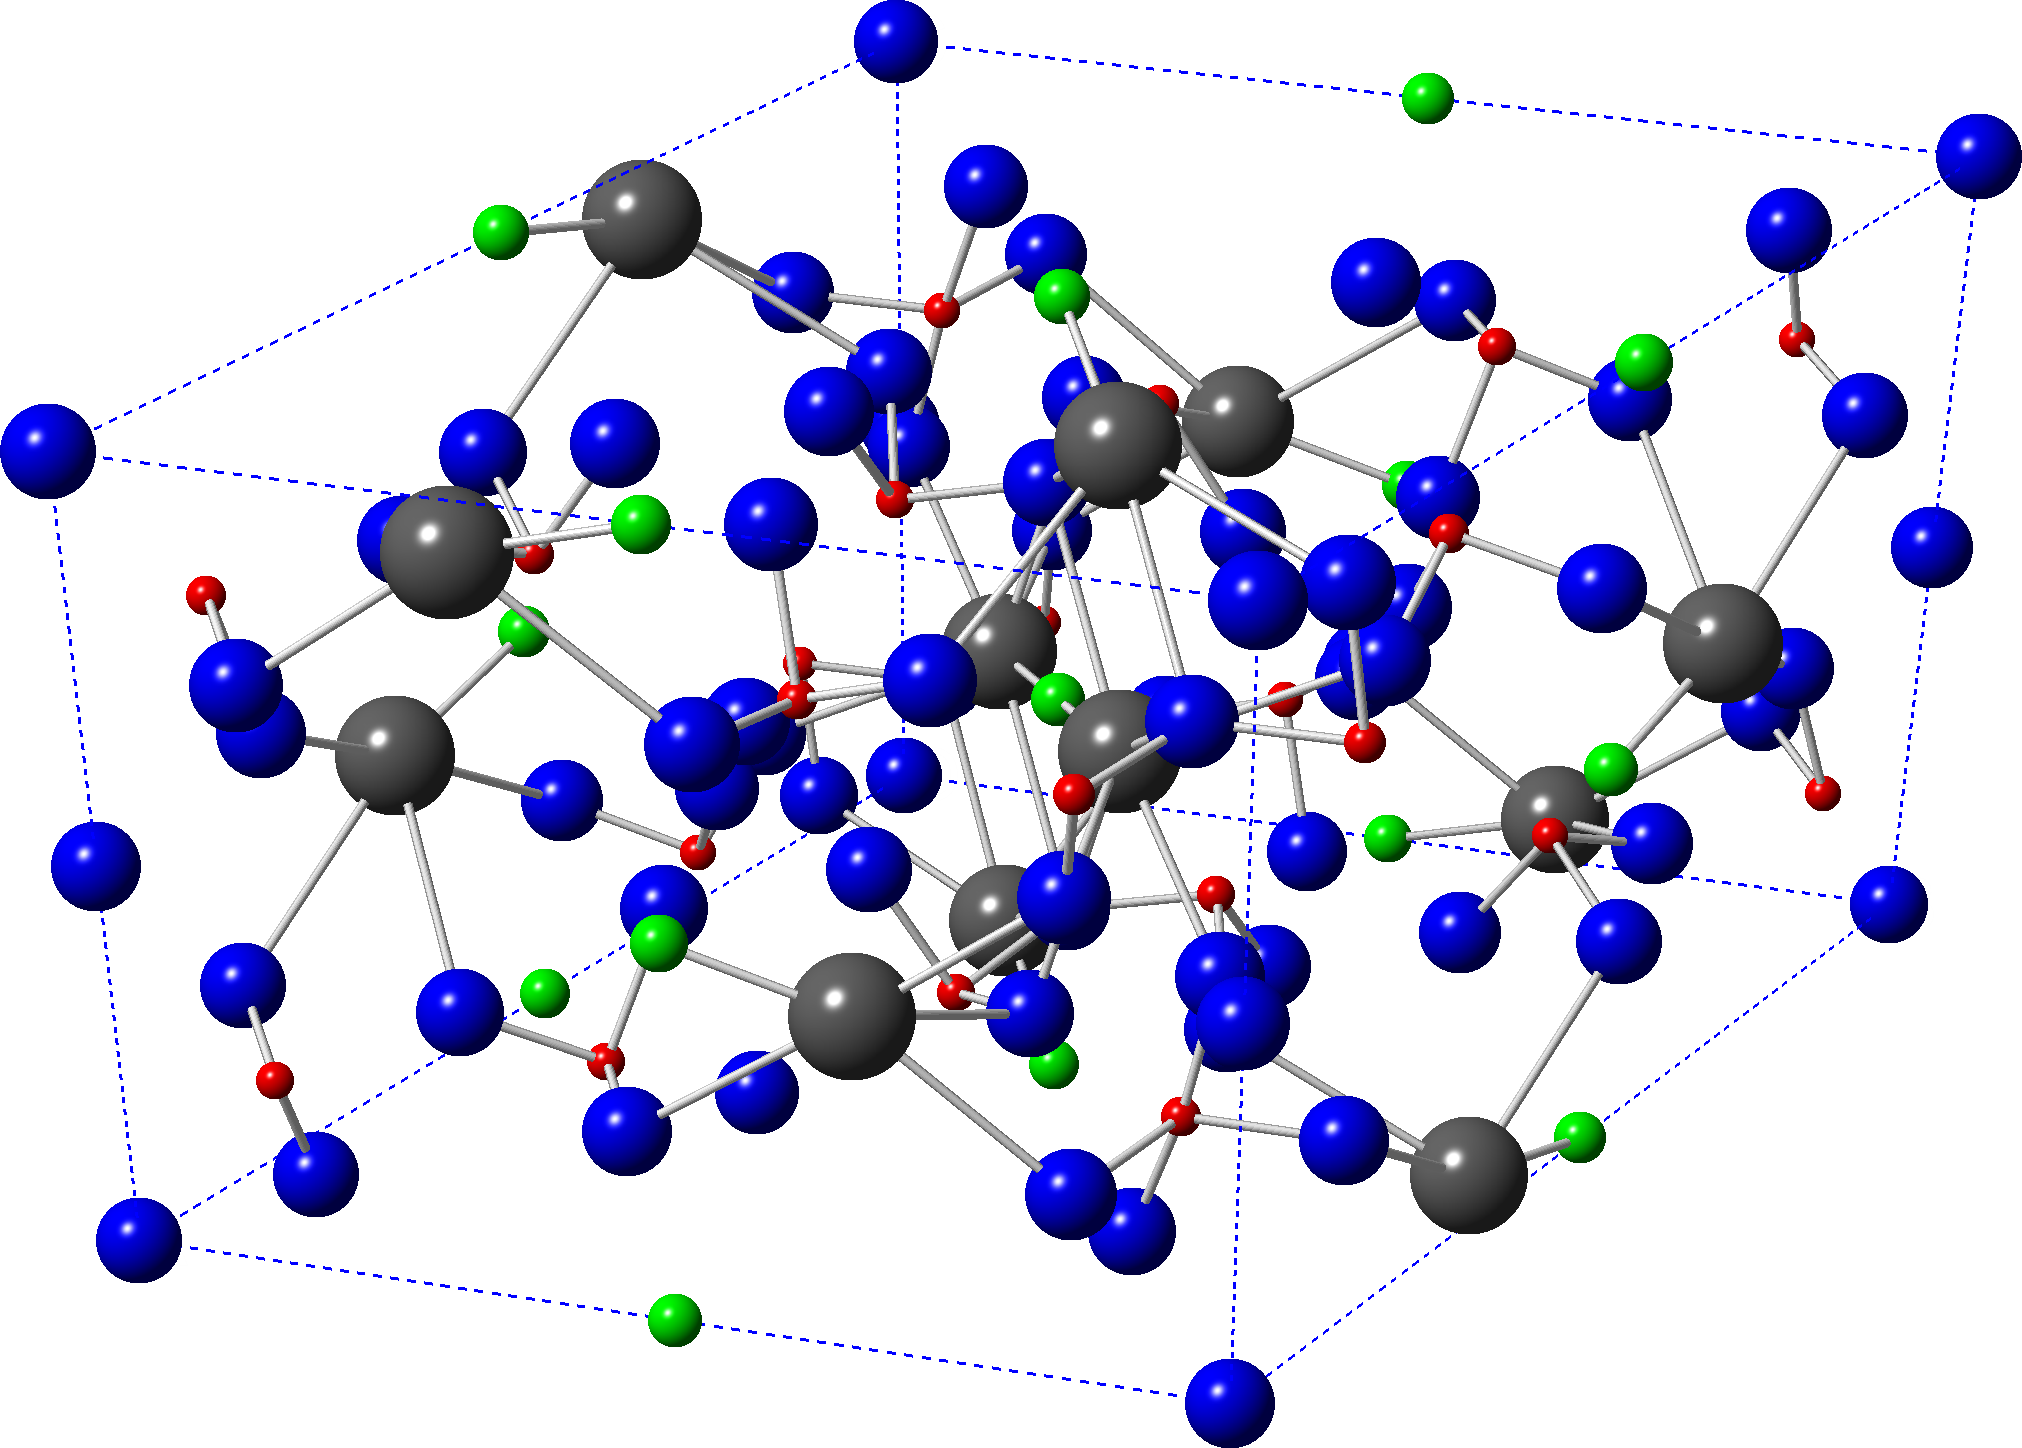
\includegraphics[height = 0.27\textwidth]{img/rgto-sol-4}%
	}{\caption{%
		\texttt{0@g1,1@f1g1,2@e1,3@b1d1f2g3}\\(在有孤立 \ce{O^{2-}}
		的前提下,\\每个 \ce{Ti^{4+}} 被 2 个 \ce{Rb+} 配位)%
	}}
\end{subfloatrow}}{\caption{“0009563”的一些解}\label{fig:9563-sol}}
\vspace{\slop{-0.6em}}
\end{figure}

\section{讨论和小结}
\subsection{关于动态剪枝的讨论}\label{ssec:prune-discus}

如第 \ref{ssec:incr-epc} 小节所述,Wyckoff 位置种类较多的空间群对于原子数稍多的
结构往往会生成极大量的可行 EPC;其内存溢出的潜在问题可以用增量生成 EPC 解决,
但其使结构测定的时间复杂度发生爆炸性增长仍是一个严重的问题。\textcite{lu1965}%
在求解 \ce{V2Ga5} 结构时筛选 EPC 的思路对我们有一定的启发:其根据对晶胞几何属性
的分析得出了各个 Wyckoff 位置之间的互斥关系。第 \ref{ssec:epc-discus} 小节指出,
可以通过在 \emph{decryst} 中引入涉及多于一个 Wyckoff 位置的占据数约束来应用
Wyckoff 位置的互斥关系;然而,这样的互斥关系在很多时候难以手工进行推导。

事实上,如果从深度优先树搜索的角度考虑,不难注意到生成 EPC 时的互斥约束也可以
放到剪枝的框架之下来理解:例如对于 \ce{V2Ga5},因为 $a$、$b$ 位置互斥,在其中
一个位置有占据时另一位置被占据的子树在搜索时就被剪掉了。在此背景之下,我们可以
沿用 \ref{ssec:epc-filter} 小节中利用原子重叠评估函数进行 EPC 筛选的思路,不再
手工推导互斥关系,而是动态地对互斥关系进行检测:在树搜索中时实时地对当前节点
所代表的(部分或全部原子的)EPC 进行针对原子重叠的统计分析或全局最优化,
并将不可能产生无碰撞晶体模型的子树剪掉。

如果要实现这样的动态剪枝,那么 EPC 的生成和(针对原子重叠而非衍射谱的)统计分析
或全局最优化将必须在同一步骤中进行,因此 \emph{decryst} 的设计和实现必须经过
大幅度的修改:在搜索过的每个节点上加入统计分析会明显增加树搜索的复杂度,
而全局最优化更是如此,因此动态剪枝必须是可选的,而且在启用动态剪枝时还必须
考虑树搜索的并行化问题,此外参数取值的遍历顺序(例如 $a_1b_1 \rightarrow
a_2b_1 \rightarrow \cdots \rightarrow a_1b_2 \rightarrow \cdots$ 和
$a_1b_1 \rightarrow a_1b_2 \rightarrow \cdots \rightarrow a_2b_1 \rightarrow
\cdots$)对算法复杂度的影响应该也是需要考虑的。不过有必要指出,在晶体学
软件中类似的情况不是只在 \emph{decryst} 里出现:例如为了将电荷反转法
(参考第 \ref{sec:reci-meth} 节)应用于衍射峰之间常有明显重叠的粉末
衍射数据,相应的算法\parencite{baerlocher2007}须要实时地对衍射峰的
划分方案进行调整,而分峰在倒空间法中原本通常是相对独立的步骤;
事实上,UACIEM\parencite{ma2004}就是一种动态分峰算法。

\subsection{其它讨论}

如第 \ref{ssec:epc-filter} 小节所述,除了在求解之后用于筛除发生原子重叠的解
模型以及在求解过程中实时排除发生重叠的晶体模型之外,本文中的原子重叠评估函数
也可以用于在求解前筛除不可能产生无重叠晶体模型的 EPC。更复杂的评估函数,例如
考虑键角、配位数、成键类型、原子链类型等等因素的那些\parencite{li2012},
从原则上看应该也可以用于类似用途,而且从实践上看肯定会有重要的意义:
例如要是能实际使用这样的评估函数,我们在求解“0000428”结构时就可以
很容易地拉开正确解和错误解在目标函数值上的差别,而在求解“0009563”
结构时也能极大地简化最后的手工(目视)筛选步骤。

从本章中大部分测试结构的求解过程可见,我们如果能自动化地实现对等价 EPC 和等价
晶体模型的检测,就能进一步提升结构测定的效率。前一问题大概可以通过按局部对称性
(site symmetry)对 Wyckoff 位置进行分组(例如 $R\bar3$ 空间群中 $d$、$e$
位置的局部对称性均为 $\bar1$),然后为对称操作可能导致的组内互变关系(例如
$R\bar3$ 空间群中 $(0, 0, 1/2)$ 平移可以使 $a/b$、$d/e$ 位置互变)
构造查找表的方式来处理。后一问题大概须要通过对某种特征性的指标进行
聚类分析来实现,而 \emph{CALYPSO}\parencite{wang2012}中的成键特征矩阵
(bond characterisation matrix)方法可能对这一指标的构造有一定的启发意义。

如第 \ref{ssec:epc-filter} 小节所述,即使在求解前筛除不可能产生无重叠晶体模型
的 EPC,并在求解中实时排除发生重叠的晶体模型,我们最后仍然可能得到发生重叠的解
模型;本人认为,发生这种现象的根本原因是某些 EPC 不能产生 $R$ 因子很小而且同时
不发生原子重叠的晶体模型,或者至少只能以很小的概率得到这样的模型。出于这一原因,
我们目前仍然须要在求解之后筛除发生重叠的解模型;另一种应该可行的思路是在目标函数
中以一种非线性的方式组合 $R$ 因子和原子重叠评估函数,从而使得目标函数值
在趋于零时被 $R$ 因子和评估函数值中较大的那个数值决定。

\subsection{本章小结}

\emph{decryst} 的设计追求简洁、灵活,而本人也希望其中的技巧可以在更多的晶体学
软件中得到应用。在现有自动化工具的配合下,用 \emph{decryst} 能简单地实现相当
复杂的求解流程:利用重原子法的求解,统计分析和全局最优化后基于 Bragg $R$
因子的等效点系组合(EPC)筛选,求解前筛除必发生原子重叠的 EPC、最优化中实时
排除存在原子重叠的晶体模型、求解后筛除仍发生原子重叠的 EPC,等等。为了演示
\emph{decryst} 的基本用法和常用技巧,本人从美国矿物学家晶体结构数据库(AMCSD)
中选取了若干个不同晶系和复杂度的测试结构,并成功地对它们进行了求解。

\begin{rquote}{0.1\textwidth}
	Almost anything in software can be implemented, sold, and even used, given
	enough determination.  There is nothing a mere scientist can say that will
	stand against the flood of a hundred million dollars.  But there is one
	quality that cannot be purchased in this way, and that is reliability.
	The price of reliability is the pursuit of the utmost simplicity.
	It is a price which the very rich find most hard to pay.
\end{rquote}
\rightline{--- C. A. R. Hoare (\cite*{hoare1981})}

% vim:ts=4:sw=4

	% Copyright (c) 2014,2016,2018 Casper Ti. Vector
% Public domain.

\chapter{结论和展望}

本人提出了一种具有通用性的晶体学碰撞检测算法框架,按照此框架让 sweep and prune%
(SAP)算法能以 $O(n\log n)$ 的时间复杂度检测晶胞中的成键关系,并提出了一种
在小晶胞中也适用的利用等效点系对称性极大降低碰撞检测复杂度的算法,最后基于以上
算法提出了一种针对晶胞中原子重叠状况的评估函数。利用以上结果,我们能在正空间法
的全局最优化步骤中高效地对晶胞中的成键关系进行检测,从而可以实时地排除存在
原子重叠的晶体模型,以及实时地进行关于配位多面体、原子键价等等的计算。
在此基础之上值得进一步探索的课题主要是上述晶体学碰撞检测算法框架在
成键关系大部分已知的结构上的应用,以及细碰撞检测正确性的证明。

基于上述机制,本人开发了 \emph{decryst} 这一套利用正空间法和等效点系组合(EPC)
法从指标化的粉末衍射数据求解晶体结构的软件,其中首次以一种一般性的方式使用
增量计算的思想来提升其计算性能,并且通过一种增量的算法生成 EPC 以降低其内存需求,
此外 \emph{decryst} 中也加入了对并行和分布式计算的支持。通过应用以增量计算为
代表的惰性计算技术,以及并行和分布式计算,\emph{decryst} 有着很高的性能;因为
EPC 互相独立且数量往往很大,\emph{decryst} 对 EPC 任务的并行化将为求解
成键关系总体未知的结构带来前所未有的机遇。在此基础之上值得进一步探索的
课题主要是更加复杂的目标函数在 \emph{decryst} 中的应用,以及对
\emph{decryst} 中全局最优化算法的进一步改进。

\emph{decryst} 的设计追求简洁、灵活,而本人也希望其中的技巧可以在更多的晶体学
软件中得到应用;在现有自动化工具的配合下,用 \emph{decryst} 能简单地实现相当
复杂的求解流程。本人以从美国矿物学家晶体结构数据库(AMCSD)中若干个不同晶系和
复杂度的测试结构为例,演示了 \emph{decryst} 的基本用法和常用技巧。在目前工作的
基础之上,主要值得进一步探索的课题是利用增量 EPC 生成算法中剪枝的思路动态地排除
不可能生成无碰撞晶体模型的 EPC,以及对等价 EPC 和等价晶体模型的自动排除。

\begin{rquote}{0.4\textwidth}
	Finally, the number of Unix installations
	has grown to 10, with more expected.
\end{rquote}
\rightline{--- Ken Thompson and Dennis Ritchie (\cite*{thompson1972})}

% vim:ts=4:sw=4


	\appendix
	\printbibliography[heading = bibintoc]
	\backmatter
	% Copyright (c) 2014,2016,2018 Casper Ti. Vector
% Public domain.

\chapter{致谢}

首先要感谢的是董成老师,因为如果没有他提出原子重叠的自动化处理这样一个极其适合我
的课题,我很难如此顺利地进行研究生期间的科研工作并完成本文。不仅如此,尽管
我和董成老师之间在不少技术问题上有明显的分歧,他不但没有阻止我投稿,而且主动要求
在我的论文\parencite{liu2017, liu2018}中不署名,甚至批准了我的提前答辩申请;
能这样做的导师在研究生导师中未必是多数,因此我衷心地感谢董成老师的高风亮节。

我也要感谢北大化学院的王颖霞老师和中科院高能所的王焕华老师,因为他们不仅分别
从化学家和物理学家的角度让我入了晶体学的门,而且在晶体学之外的不少方面给了我
很多帮助。还要感谢的是北大数学院的范后宏老师以及 \emph{Tensor Geometry}%
\parencite{dodson1991}的作者,因为前者开设的线性代数课程和后者
关于同一主题的阐述使我对代数和几何之间关系的理解有了质的飞跃,
而数形结合的思路正是解决原子重叠问题的数学基础。

感谢 Ken Thompson、Dennis Ritchie 等等 Unix 先驱以及 Daniel J.\ Bernstein、%
Laurent Bercot 等等 Unix 精神继承者,因为他们所提倡的 Unix 哲学“do one thing
and do it well”\parencite{salus1994}使我不仅能以很高的效率完成 \emph{decryst}
和其它的项目中的编程任务,而且能以更深刻的眼光来审视学习和生活中的问题,
这样的影响是无价的。我也要感谢北大 Linux 俱乐部和其它一些开源社区,
因为它们提供的平台使我接触了来自各家的技术观点,这也是无价的。

感谢 \emph{decryst} 的测试用户,\emph{decryst} 的文档质量在他们的意见和建议之下
得到了极大的提升;感谢 \TeX{}$\big/$\LaTeX{} 社区的许多人,他们的工作极大地
简化了本文的撰写。最后也要感谢 AMCSD 数据库\parencite{downs2003}%
和 Bilbao 服务器\parencite{aroyo2006}的作者在开放获取的精神之下
提供了宝贵的数据和一些有用的工具,以及感谢 \emph{GNU Parallel}%
\parencite{tange2011}作者的工作极大地方便了本文中一些数据的处理。
本文中的相关工作受到了国家自然科学基金(批准号:21271183)
和国家重点研发计划(批准号:2017YFA0302903)的资助。

\begin{rquote}{0.2\textwidth}
	我用一种悲悯的心情来写剧中人物的争执。我诚恳地祈望着
	看戏的人们也以一种悲悯的眼来俯视这群地上的人们。
\end{rquote}
\rightline{——《\emph{〈雷雨〉序}》\parencite{cao1936}}

% vim:ts=4:sw=4

	% Copyright (c) 2018 Casper Ti. Vector
% Public domain.

\chapter{作者简历和研究成果目录}

\section*{作者简历}
\begin{itemize}[leftmargin = \parindent]
\item 2008 年 9 月 -- 2009 年 7 月在北京大学医学部药学院学习。
\item 2009 年 9 月 -- 2013 年 7 月在北京大学化学与分子工程学院获得学士学位。
\item 2013 年 9 月 -- 2014 年 7 月在家报考中国科学院物理研究所。
\item 2014 年 9 月至今在中国科学院物理研究所攻读博士学位。
\end{itemize}

\section*{已发表或正式接受的学术论文}
\defbibenvironment{publications}%
	{\begin{itemize}[leftmargin = \parindent]}{\end{itemize}}{\item}
\begin{refsection}
\renewcommand*{\bibfont}{}
\nocite{liu2017, liu2018}
\begin{refcontext}[sorting = none]
\printbibliography[heading = none, env = publications]
\end{refcontext}
\end{refsection}

\section*{参与的研究项目及获奖情况}
\begin{itemize}[leftmargin = \parindent]
\item 参与国家自然科学基金项目(批准号:21271183)
	“层状过渡金属硫属化合物的合成、晶体结构和超导电性研究”。
\item 参与国家重点研发计划项目(批准号:2017YFA0302903)
	“关联电子的量子效应及调控”。
\item 2017 年 12 月获中国科学院物理研究所所长奖学金表彰奖。
\end{itemize}

% vim:ts=4:sw=4

	\cleardoublepage
\end{document}

% vim:ts=4:sw=4
